\documentclass[12pt,a4paper]{article}

% ============================================================
% Préambule
% ============================================================
\usepackage[utf8]{inputenc}
\usepackage[T1]{fontenc}
\usepackage{lmodern}
\usepackage[provide=*]{babel}

\usepackage[a4paper,margin=2.5cm]{geometry}
\linespread{1.15}
\usepackage{fancyhdr}
\usepackage{titlesec}
\usepackage{enumitem}

\usepackage{graphicx}
\usepackage{booktabs}
\usepackage{longtable}
\usepackage{xcolor}
\usepackage{tikz}
\usetikzlibrary{arrows.meta,positioning}
\usepackage[listings]{tcolorbox}
\tcbuselibrary{skins}
\lstset{
  basicstyle=\ttfamily\footnotesize,
  breaklines=true,
  frame=single,
  framesep=4pt,
  backgroundcolor=\color{gray!8},
  keywordstyle=\color{blue!70!black},
  commentstyle=\color{green!45!black},
  stringstyle=\color{red!60!black},
  showstringspaces=false,
  tabsize=2,
  columns=fullflexible
}

\usepackage[colorlinks=true,linkcolor=blue!55!black,urlcolor=blue!55!black,citecolor=blue!55!black]{hyperref}

\pagestyle{fancy}
\fancyhf{}
\fancyhead[L]{\small DevOps Central Platform}
\fancyhead[R]{\small Rapport technique détaillé}
\fancyfoot[C]{\thepage}
\renewcommand{\headrulewidth}{0.4pt}

\titleformat{\section}{\Large\bfseries}{\thesection}{1em}{}
\titleformat{\subsection}{\large\bfseries}{\thesubsection}{1em}{}
\titleformat{\subsubsection}{\normalsize\bfseries}{\thesubsubsection}{1em}{}
\titlespacing*{\section}{0pt}{2.4ex plus .5ex}{1.3ex}
\titlespacing*{\subsection}{0pt}{2.0ex plus .4ex}{1.0ex}

\setlength{\parskip}{0.55em}
\setlength{\parindent}{0pt}
\sloppy
\hbadness=10000  % silence les warnings Underfull cosmétiques

% ---------- Boîte « Pourquoi ce choix » ----------
\newtcolorbox{whybox}[1][]{
  colback=blue!4,colframe=blue!55!black,boxrule=0.6pt,
  arc=1.5mm,left=6pt,right=6pt,top=4pt,bottom=4pt,
  title={Pourquoi ce choix},fonttitle=\bfseries,#1
}

% ---------- Boîte « Capture à insérer » ----------
\newcounter{capturecount}
\newcommand{\capturebox}[2]{%
\par\vspace{4mm}
\begin{tcolorbox}[enhanced,colback=yellow!5,colframe=black!55,boxrule=0.7pt,
  borderline={0.7pt}{0pt}{black!40,dashed},
  arc=2mm,left=6pt,right=6pt,top=7pt,bottom=7pt]
\centering
{\normalsize\sffamily\bfseries CAPTURE À INSÉRER \textbar\ n°\,\stepcounter{capturecount}\thecapturecount}\\[3pt]
{\large\texttt{images/#2}}\\[7pt]
\begin{minipage}{0.94\linewidth}\centering\itshape #1\end{minipage}
\end{tcolorbox}
\par\vspace{2mm}}

\begin{document}

% ============================================================
% Page de garde
% ============================================================
\begin{titlepage}
  \centering
  \vspace*{1.6cm}
  {\Huge\bfseries DevOps Central Platform\par}
  \vspace{0.6cm}
  {\LARGE Rapport technique détaillé\par}
  \vspace{0.4cm}
  {\Large Analyse exhaustive des outils et technologies\par}
  \vspace{1cm}
  {\large Infrastructure as Code · Configuration · Conteneurisation · Kubernetes\\
  Microservices FastAPI · Secrets Vault · CI/CD GitHub Actions · DevSecOps\\
  GitOps ArgoCD · Observabilité Prometheus / Grafana / ELK · SLO\par}
  \vfill
  {\large Gadour\par}
  \vspace{0.4cm}
  {\large \today\par}
  \vfill
  {\footnotesize Analyse issue de la lecture intégrale du code source actif :\par
  \texttt{terraform/ · ansible/ · app/ · k8s/ · scripts/ · .github/workflows/}\par
  \vspace{4mm}
  Les emplacements de captures d'écran sont matérialisés par des cadres jaunes numérotés\par
  indiquant le fichier attendu sous \texttt{images/}.\par}
\end{titlepage}

\tableofcontents
\clearpage

% ============================================================
\part{Cadre du projet}
% ============================================================

% ------------------------------------------------------------
\section{Introduction}
% ------------------------------------------------------------

\textbf{DevOps Central Platform} est une plateforme d'infrastructure DevOps de bout en bout construite autour de trois microservices \texttt{FastAPI} (\emph{Users}, \emph{Products}, \emph{Orders}). L'application est un support volontairement simple : l'objectif réel du projet est de maîtriser la chaîne DevOps moderne telle que pratiquée en entreprise --- provisionnement des serveurs, configuration automatisée, conteneurisation, orchestration Kubernetes, sécurité intégrée au pipeline (DevSecOps), déploiement GitOps et observabilité complète (métriques \emph{et} logs centralisés).

Le projet tourne sur un \textbf{homelab libvirt/KVM}. Aucun service cloud facturé n'est utilisé ; la plateforme entière est reproductible sur une station personnelle Linux, tout en restant structurellement proche d'une production réelle (VMs, SSH, systemd, kernel, cluster Kubernetes multi-nœuds).

Ce rapport documente \textbf{chaque outil et technologie présents dans le dépôt} : ce qu'il fait précisément ici, comment il est configuré (avec les valeurs exactes du code), pourquoi il a été choisi face aux alternatives, et où en observer le fonctionnement en démonstration (emplacements de captures prévus).

\subsection{La question fondatrice}
Le projet répond à une question simple : \emph{comment une équipe d'ingénierie fait-elle tourner une application en production de façon fiable, sécurisée et observable, sans intervention manuelle ?}

Chaque brique du rapport apporte un élément de réponse :
\begin{itemize}[itemsep=1pt]
  \item \emph{de façon reproductible} $\rightarrow$ Terraform, cloud-init, Ansible ;
  \item \emph{fiable} $\rightarrow$ Kubernetes, probes, HPA, PDB, auto-réparation ;
  \item \emph{sécurisée} $\rightarrow$ Gitleaks, Trivy, pip-audit, Vault, NetworkPolicies, PSA restricted ;
  \item \emph{observable} $\rightarrow$ Prometheus, AlertManager, Grafana, ELK ;
  \item \emph{sans intervention manuelle} $\rightarrow$ GitHub Actions + ArgoCD (GitOps).
\end{itemize}

\subsection{Philosophie : documenter aussi les échecs}
Le projet ne se limite pas à faire fonctionner l'architecture : il documente comment elle \textbf{échoue en pratique} et comment ces échecs se corrigent. Les alertes plateforme (OOMKill, HPA bloqué au maximum, saturation mémoire) correspondent à des incidents réellement rencontrés pendant le développement --- chaque règle d'alerte porte l'étiquette \texttt{incident="N"} qui renvoie au post-mortem correspondant.

% ------------------------------------------------------------
\section{Méthodologie et périmètre de l'analyse}
% ------------------------------------------------------------

\subsection{Sources analysées}
Toutes les informations proviennent de la lecture directe du code source actif :

\begin{longtable}{@{}p{4.6cm}p{9.6cm}@{}}
\toprule
\textbf{Répertoire / fichier} & \textbf{Contenu analysé} \\
\midrule
\endhead
\texttt{terraform/} & main.tf, variables.tf, outputs.tf, backend.tf, templates cloud-init et inventaire \\
\texttt{ansible/} & playbook.yml, ansible.cfg, requirements.yml, group\_vars/all.yml, rôles docker, k8s\_common, k8s\_master, k8s\_worker, k8s\_reset \\
\texttt{app/} & main.py ×3, Dockerfile ×3, requirements.txt ×4, shared/ (vault\_client.py, log\_config.py, config.py) \\
\texttt{k8s/apps/} & base/, users/, products/, orders/ + overlays dev/staging/prod \\
\texttt{k8s/monitoring/} & prometheus/, alertmanager/, grafana/, elk/, kubelet/, kube-state-metrics/ \\
\texttt{k8s/argocd/} & install/ + 12 Applications + AppProject \\
\texttt{k8s/vault/} & manifests.yaml, vault-policy.hcl, template de Secret \\
\texttt{k8s/policies/} & politiques conftest Rego + Kyverno \\
\texttt{.github/workflows/}\\ \texttt{ci-cd.yml} & pipeline complet (447 lignes) \\
\texttt{scripts/} & validate-platform.sh, validate-security.sh, generate-inventory.sh, bootstrap-*.sh, smoke-test.sh, stress-hpa.sh, stress-panel.py \\
\texttt{tests/} & test\_services.py (pytest) \\
\texttt{racine} & .pre-commit-config.yaml, .gitleaks.toml, .gitignore, .dockerignore, .env.example \\
\bottomrule
\end{longtable}

\begin{whybox}
Le dossier \texttt{docs/} a été \textbf{volontairement exclu} de l'analyse : ses spécifications sont obsolètes par rapport au code. Le code est la seule source de vérité --- c'est aussi la philosophie GitOps défendue par le projet lui-même.
\end{whybox}

\subsection{Convention des emplacements de capture}
Tout au long du rapport, des cadres jaunes numérotés indiquent les démonstrations à capturer :

\capturebox{Exemple d'emplacement de capture. Remplacer ce cadre par :
\texttt{\textbackslash includegraphics[width=\textbackslash linewidth]\{images/nom.png\}}
légendée selon la description ci-dessus.}{exemple-emplacement.png}

Chaque cadre précise : le \textbf{nom de fichier attendu} (à placer dans \texttt{images/}), et la \textbf{description exacte} de ce qu'il faut montrer (commande à lancer, écran à viser).

% ------------------------------------------------------------
\section{Vue d'ensemble de l'architecture}
% ------------------------------------------------------------

\subsection{Les six dimensions de la plateforme}

\begin{enumerate}[itemsep=2pt]
  \item \textbf{Infrastructure as Code} --- création automatisée et reproductible des serveurs (Terraform) ;
  \item \textbf{Configuration automatisée} --- installation et paramétrage des serveurs et du cluster (cloud-init, Ansible) ;
  \item \textbf{Conteneurisation \& orchestration} --- empaquetage et exécution orchestrée (Docker, containerd, Kubernetes, Calico) ;
  \item \textbf{Sécurité intégrée (DevSecOps)} --- scan du code, des dépendances et des images, gestion dynamique des secrets, politiques d'admission (Gitleaks, Trivy, pip-audit, Vault, conftest, Kyverno) ;
  \item \textbf{Déploiement automatisé (GitOps)} --- synchronisation continue Git $\leftrightarrow$ cluster (GitHub Actions, ArgoCD) ;
  \item \textbf{Observabilité complète} --- métriques et logs centralisés, alerting SLO (Prometheus, AlertManager, Grafana, ELK).
\end{enumerate}

\subsection{Flux de bout en bout}

\begin{center}
\resizebox{\textwidth}{!}{%
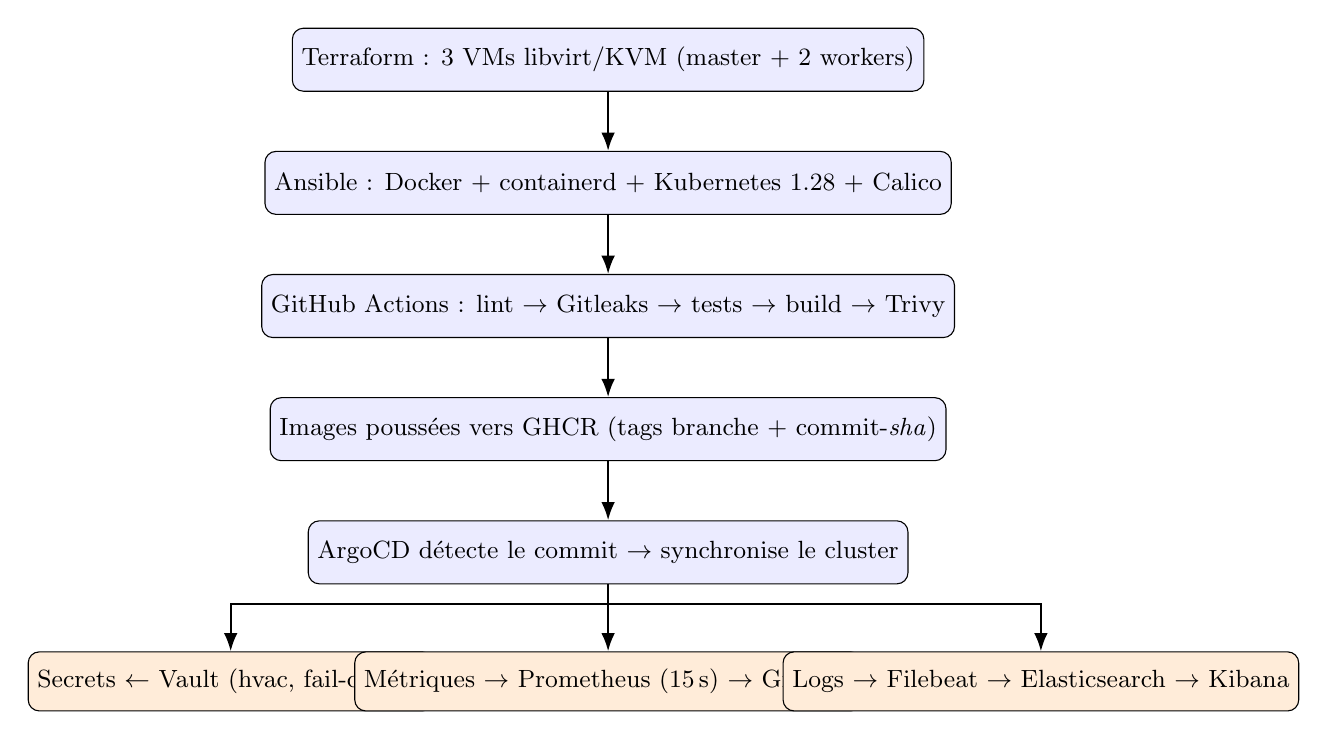
\begin{tikzpicture}[
  node distance=0.75cm and 0.9cm,
  box/.style={draw, rounded corners, fill=blue!8, minimum width=5.6cm, minimum height=0.8cm, align=center, font=\small},
  side/.style={draw, rounded corners, fill=orange!15, minimum width=3.9cm, minimum height=0.75cm, align=center, font=\small},
  arr/.style={-{Latex}, thick}
]
  \node[box] (tf) {Terraform : 3 VMs libvirt/KVM (master + 2 workers)};
  \node[box, below=of tf] (an) {Ansible : Docker + containerd + Kubernetes 1.28 + Calico};
  \node[box, below=of an] (ci) {GitHub Actions : lint $\rightarrow$ Gitleaks $\rightarrow$ tests $\rightarrow$ build $\rightarrow$ Trivy};
  \node[box, below=of ci] (ghcr) {Images poussées vers GHCR (tags branche + commit-\textit{sha})};
  \node[box, below=of ghcr] (argo) {ArgoCD détecte le commit $\rightarrow$ synchronise le cluster};
  \node[side, below left=0.85cm and -1.6cm of argo] (vault) {Secrets $\leftarrow$ Vault (hvac, fail-closed)};
  \node[side, below=0.85cm of argo] (prom) {Métriques $\rightarrow$ Prometheus (15\,s) $\rightarrow$ Grafana};
  \node[side, below right=0.85cm and -1.6cm of argo] (elk) {Logs $\rightarrow$ Filebeat $\rightarrow$ Elasticsearch $\rightarrow$ Kibana};

  \draw[arr] (tf) -- (an);
  \draw[arr] (an) -- (ci);
  \draw[arr] (ci) -- (ghcr);
  \draw[arr] (ghcr) -- (argo);
  \draw[arr] (argo.south) -- ++(0,-0.25) -| (vault.north);
  \draw[arr] (argo.south) -- (prom.north);
  \draw[arr] (argo.south) -- ++(0,-0.25) -| (elk.north);
\end{tikzpicture}%
}
\end{center}

\subsection{Inventaire rapide des technologies}
Le tableau final (\S\ref{sec:recap}) recense \textbf{plus de quarante outils}, chacun détaillé dans une section dédiée : hyperviseur, IaC, configuration, runtime conteneurs, CNI, framework applicatif, bibliothèques Python, gestionnaire de secrets, registre, six outils de scan/qualité, moteur GitOps, quatre composants de monitoring et quatre composants ELK.

\capturebox{Schéma d'architecture général redessiné ou photographié depuis un tableau blanc / outil de diagramme : les 3 VMs, le cluster K8s, les namespaces (devops-platform, monitoring, vault, argocd), les flux CI et GitOps.}{architecture-globale.png}

\clearpage
% ------------------------------------------------------------
\section{Fiches d'identité des outils majeurs}
% ------------------------------------------------------------

Références rapides --- le détail de chaque outil figure dans sa section dédiée.

\begin{tcolorbox}[colback=gray!4,colframe=black!60,arc=1.5mm,title={\bfseries Terraform},fonttitle=\bfseries]
\small
\begin{tabular}{@{}p{2.4cm}p{10.8cm}@{}}
Catégorie & Infrastructure as Code \\
Version & \textasciitilde 1.5 (CI : 1.5.7) ; providers libvirt 0.9.8 / local 2.9.0 \\
Fichiers & terraform/main.tf · variables.tf · outputs.tf · backend.tf · templates \\
Commande clé & \texttt{terraform plan/apply} ; \texttt{-target=local\_file.} \texttt{ansible\_inventory} \\
Succès mesuré par & 3 domains Ready + inventaire régénéré sans divergence \\
Section & \S Terraform \\
\end{tabular}
\end{tcolorbox}

\begin{tcolorbox}[colback=gray!4,colframe=black!60,arc=1.5mm,title={\bfseries Ansible},fonttitle=\bfseries]
\small
\begin{tabular}{@{}p{2.4cm}p{10.8cm}@{}}
Catégorie & Configuration management agentless \\
Version & core (repo Ubuntu) + community.general 8.0.0 \\
Fichiers & playbook.yml · ansible.cfg · group\_vars/all.yml · roles/* (5 rôles) \\
Commande clé & \texttt{ansible-playbook playbook.yml} (+ tags docker/k8s/master/worker) \\
Succès mesuré par & PLAY RECAP rc=0, nœuds Ready, dpkg hold actifs \\
Section & \S Ansible \\
\end{tabular}
\end{tcolorbox}

\begin{tcolorbox}[colback=gray!4,colframe=black!60,arc=1.5mm,title={\bfseries Docker / containerd},fonttitle=\bfseries]
\small
\begin{tabular}{@{}p{2.4cm}p{10.8cm}@{}}
Catégorie & Build images OCI / runtime CRI \\
Base & python:3.11-slim multi-stage, non-root appuser, HEALTHCHECK \\
Fichiers & app/*/Dockerfile · .dockerignore · rôle ansible docker \\
Commande clé & \texttt{docker build -f app/\$svc/Dockerfile app/} ; \texttt{crictl ps} \\
Succès mesuré par & images $<$150 Mo healthy, SystemdCgroup=true partout \\
Section & \S Docker · \S containerd \\
\end{tabular}
\end{tcolorbox}

\begin{tcolorbox}[colback=gray!4,colframe=black!60,arc=1.5mm,title={\bfseries Kubernetes + Calico},fonttitle=\bfseries]
\small
\begin{tabular}{@{}p{2.4cm}p{10.8cm}@{}}
Catégorie & Orchestration / CNI \\
Version & 1.28 épinglée + held ; Calico v3.26.1 (opérateur Tigera) \\
Fichiers & k8s/apps/** · group\_vars/all.yml · rôles k8s\_* \\
Commande clé & \texttt{kubectl get nodes -o wide} · \texttt{apply -k overlays/prod} \\
Succès mesuré par & nodes Ready, netpol effectives, HPA fonctionnel \\
Section & \S Kubernetes · \S Kustomize \\
\end{tabular}
\end{tcolorbox}

\begin{tcolorbox}[colback=gray!4,colframe=black!60,arc=1.5mm,title={\bfseries Vault + hvac},fonttitle=\bfseries]
\small
\begin{tabular}{@{}p{2.4cm}p{10.8cm}@{}}
Catégorie & Gestion dynamique des secrets \\
Version & hashicorp/vault:1.15.2 (dev mode) · hvac==2.1.0 \\
Fichiers & k8s/vault/manifests.yaml · vault-policy.hcl · shared/vault\_client.py \\
Commande clé & \texttt{vault kv get secret/devops-platform/users-service} \\
Succès mesuré par & readyz 200, rotation bootstrap sans fuite argv/disk/git \\
Section & \S Vault \\
\end{tabular}
\end{tcolorbox}

\begin{tcolorbox}[colback=gray!4,colframe=black!60,arc=1.5mm,title={\bfseries GitHub Actions + GHCR + ArgoCD},fonttitle=\bfseries]
\small
\begin{tabular}{@{}p{2.4cm}p{10.8cm}@{}}
Catégorie & CI/CD push + GitOps pull \\
Versions & actions v4/v5 · trivy-action v0.24.0 · ArgoCD v2.7.16 · kustomize 5.4.3 \\
Fichiers & .github/workflows/ci-cd.yml · k8s/argocd/{install,applications} \\
Commande clé & \texttt{git push} $\rightarrow$ run CI ; deploy = dispatch manuel uniquement \\
Succès mesuré par & runs verts, Applications Synced+Healthy, rollback = git revert \\
Section & \S GitHub Actions · \S ArgoCD \\
\end{tabular}
\end{tcolorbox}

\begin{tcolorbox}[colback=gray!4,colframe=black!60,arc=1.5mm,title={\bfseries Stack observabilité},fonttitle=\bfseries]
\small
\begin{tabular}{@{}p{2.4cm}p{10.8cm}@{}}
Catégorie & Métriques + alerting + dashboards + logs \\
Versions & Prometheus Operator 0.74/v2.51 · Alertmanager 0.27 · Grafana 11.1 · ELK 8.14 · KSM 2.10.1 \\
Fichiers & k8s/monitoring/** (prometheus, alertmanager, grafana, elk) \\
Commande clé & \texttt{kubectl get servicemonitor,prometheusrule -n monitoring} \\
Succès mesuré par & targets UP, alertes SLO armées, logs dans Kibana, 4 dashboards provisionnés \\
Section & \S Observabilité \\
\end{tabular}
\end{tcolorbox}

\capturebox{Montage d'écran (collage) des interfaces principales côte à côte : GHCR packages, UI ArgoCD, Grafana, Kibana.}{fiches-collage-ui.png}


\subsection{Inventaire des namespaces}
\begin{longtable}{@{}p{3.4cm}p{2.6cm}p{8.0cm}@{}}
\toprule
\textbf{Namespace} & \textbf{PSA} & \textbf{Contenu} \\
\midrule
\endhead
devops-platform & restricted & 3 services (SA dédiés, HPA, PDB, netpol), quotas, Secret vault-root-token \\
monitoring & restricted & Prometheus, AlertManager, Grafana+sidecar, ES, Filebeat DS, Logstash, Kibana, KSM, ServiceMonitors, rules SLO, 4 dashboards CM \\
vault & baseline & Vault 1.15.2 dev-mode + Job setup (IPC\_LOCK requis) \\
argocd & --- & ArgoCD v2.7.16 complet + Applications \\
kube-system / calico-system & --- & composants cluster (hors périmètre applicatif) \\
\bottomrule
\end{longtable}

\subsection{Comparaison des environnements}
\begin{longtable}{@{}p{3.0cm}p{3.6cm}p{3.6cm}p{3.8cm}@{}}
\toprule
\textbf{Aspect} & \textbf{dev} & \textbf{staging} & \textbf{prod} \\
\midrule
\endhead
Namespace & devops-platform & staging & production \\
Réplicas & 1 & 2 (base) & 3 \\
PDB minAvailable & 1 & 1 & 2 \\
Images & latest & latest & digest sha256 par CD \\
Secrets & replis dev actifs & Vault réel & Vault réel fail-closed \\
Déclenchement & push branche & sync ArgoCD manuel possible & dispatch GitHub uniquement \\
\bottomrule
\end{longtable}

\begin{whybox}
Trois overlays pour trois postures : en dev on privilégie la vitesse (réplica unique, replis secrets), en prod la disponibilité (3 réplicas, PDB resserré) et l'immuabilité (digests épinglés). La différence tient dans quelques lignes de patch --- tout le reste est partagé depuis base/.
\end{whybox}

\capturebox{\texttt{kustomize build k8s/apps/overlays/dev | grep -c 'replicas: 1'} vs prod : comparaison côte à côte des rendus.}{overlays-diff-devprod.png}

\capturebox{\texttt{kubectl get ns --show-labels} : les quatre namespaces avec leurs labels PSA.}{namespaces-psa.png}

% ------------------------------------------------------------
\section{Topologie réseau et dimensionnement}
% ------------------------------------------------------------

\subsection{Réseau virtuel}
Réseau libvirt dédié créé par Terraform :

\begin{itemize}[itemsep=1pt]
  \item nom : \texttt{devops-platform-net} --- domaine DNS local : \texttt{devops.local} ;
  \item mode : isolé avec NAT vers l'extérieur ;
  \item DHCP : de \texttt{192.168.56.100} à \texttt{192.168.56.200} (les nœuds eux-mêmes sont en IP statiques hors de cette plage) ;
  \item sous-réseau : \texttt{192.168.56.0/24} --- validations Terraform : CIDR valide + plage RFC1918 obligatoire ;
  \item relais DNS vers \texttt{1.1.1.1} et \texttt{8.8.8.8}.
\end{itemize}

Plan d'adressage des nœuds :

\begin{table}[h!]
\centering
\begin{tabular}{@{}llll@{}}
\toprule
\textbf{Nœud} & \textbf{IP statique} & \textbf{Rôle cluster} & \textbf{Dimensionnement} \\
\midrule
master-01 & 192.168.56.10 & control-plane & 2 vCPU / 4 Go / 20 Go qcow2 \\
worker-01 & 192.168.56.11 & worker & 2 vCPU / 4 Go / 20 Go qcow2 \\
worker-02 & 192.168.56.12 & worker & 2 vCPU / 4 Go / 20 Go qcow2 \\
\bottomrule
\end{tabular}
\caption{Topologie par défaut (worker\_count paramétrable de 1 à 32)}
\end{table}

\subsection{Décision de dimensionnement documentée}
Les variables Terraform fixent \texttt{vm\_memory\_mb = 4096} avec un commentaire explicite : à 2048 Mo, la pile complète (ELK + ArgoCD + supervision) fait basculer le kubelet en \texttt{NodeStatusUnknown} sous pression mémoire. Ce type de décision \emph{justifiée par incident} traverse tout le projet.

\subsection{Cohérence des plans d'adressage}
Trois plans coexistent sans conflit : réseau des VMs (\texttt{192.168.56.0/24}), CIDR pods (\texttt{192.168.0.0/16}), CIDR services (\texttt{10.96.0.0/12}). La séparation stricte pods/services/nœuds est un pré-requis kubeadm classique.

\capturebox{Sortie de \texttt{virsh net-dumpxml devops-platform-net} ou vue network de virt-manager montrant le réseau NAT, la plage DHCP et les interfaces des 3 VMs.}{reseau-libvirt.png}

\capturebox{Écran virt-manager / \texttt{virsh list --all} + \texttt{virsh dominfo} pour chaque nœud montrant vCPU, RAM et disque alloués.}{vms-topologie.png}

\capturebox{Depuis master-01 : \texttt{ip addr show enp1s0} et \texttt{ping worker-01} prouvant l'adressage statique et le DNS interne.}{ip-statique-dns.png}

% ============================================================
\part{Infrastructure as Code et configuration}
% ============================================================

% ------------------------------------------------------------
\section{Libvirt/KVM --- l'hyperviseur de l'homelab}
% ------------------------------------------------------------

\subsection{Présentation générale}
KVM (Kernel-based Virtual Machine) est l'hyperviseur intégré au noyau Linux ; libvirt est son API de management standard (VMs, réseaux, stockage). Ensemble ils constituent la stack de virtualisation open-source de référence sur hôte Linux.

\subsection{Rôle dans le projet}
Fournir trois vraies machines virtuelles Ubuntu Server 22.04 formant le socle du cluster Kubernetes :
\begin{itemize}[itemsep=1pt]
  \item machines type \textbf{q35} (chipset moderne PCI-E), firmware HVM, archi x86\_64 ;
  \item disques \textbf{qcow2} clonés depuis une image de base (\texttt{ubuntu-22.04-server-} \texttt{cloudimg-amd64.img}) --- copie-on-write : chaque nœud ne consomme que ses deltas ;
  \item CD-ROM \texttt{cloud-init} par nœud (user-data, meta-data, network-config) ;
  \item carte réseau \texttt{virtio} (performances paravirtualisées) branchée sur le réseau dédié ;
  \item console série pty + VNC écoutant sur 127.0.0.1 uniquement.
\end{itemize}

\begin{whybox}
KVM/libvirt offre de \emph{vraies} VM Linux --- kernel réel, systemd, SSH --- sans coût cloud ni quotas, et sans les limitations des conteneurs-in-conteneurs. Le même workflow qu'en entreprise (provisionner, SSH-er, configurer) s'apprend chez soi gratuitement. Le provider Terraform dmacvicar/libvirt pilote le tout déclarativement : changer \texttt{worker\_count = 4} puis \texttt{apply} suffit à agrandir l'infra.
\end{whybox}

\subsection{Alternatives envisagées}
\begin{tabular}{@{}lp{10.5cm}@{}}
\toprule
\textbf{Alternative} & \textbf{Raison du rejet} \\
\midrule
VirtualBox & Provider Terraform moins mature, performances inférieures \\
Cloud public (AWS/GCP) & Coût et facturation permanents --- contre-productif pour un lab \\
kind/minikube & Cluster en conteneur unique : pas de vrai multi-nœuds, pas d'apprentissage réseau/systemd \\
Vagrant & Couche redondante dès que Terraform pilote déjà libvirt \\
\bottomrule
\end{tabular}

\subsection{Captures de démonstration}
\capturebox{\texttt{virsh list --all} montrant les 3 domaines en running + \texttt{virsh dumpxml master-01} extraits memory/vcpu.}{kvm-virsh-list.png}

\capturebox{Console VNC de master-01 au boot : messages kernel + prompt de login Ubuntu 22.04.}{kvm-console-boot.png}

\capturebox{\texttt{qemu-img info} de l'image de base et d'un volume nœud montrant format qcow2, taille virtuelle vs réelle (copie-on-write visible).}{kvm-qcow2-info.png}

% ------------------------------------------------------------
\section{cloud-init --- provisionnement et durcissement au boot}
% ------------------------------------------------------------

\subsection{Présentation générale}
cloud-init est le standard de facto du premier démarrage des instances (toutes les images cloud publiques le parlent). Il applique une configuration YAML déclarative au boot : utilisateurs, clés SSH, paquets, scripts finaux.

\subsection{Rôle dans le projet}
Chaque VM reçoit un disque cloud-init généré par Terraform depuis le template \texttt{cloud-init.tpl} :

\begin{lstlisting}[caption={Template cloud-init --- durcissement appliqué avant toute autre étape}]
ssh_pwauth: false
disable_root: true

users:
  - name: devops
    sudo:
      - ALL=(ALL) PASSWD: /usr/bin/kubeadm,
        /usr/bin/kubelet,
        systemctl restart kubelet/containerd/docker
    shell: /bin/bash

growpart: {mode: auto, devices: ['/']}
resize_rootfs: true

package_update: true
package_upgrade: true
packages: [fail2ban]

runcmd:
  - sed -i 's/^#\?PermitRootLogin.*/PermitRootLogin no/' /etc/ssh/sshd_config
  - sed -i 's/^#\?PasswordAuthentication.*/PasswordAuthentication no/' /etc/ssh/sshd_config
  - sed -i 's/^#\?PubkeyAuthentication.*/PubkeyAuthentication yes/' /etc/ssh/sshd_config
  - systemctl restart ssh || systemctl restart sshd
\end{lstlisting}

Trois familles de mesures sont appliquées dès ce premier boot.

La première concerne l'accès : l'utilisateur \texttt{devops} dispose d'un sudo \textbf{restreint par liste blanche} (uniquement kubeadm, kubelet et le redémarrage de quelques services) --- l'ancien NOPASSWD trop large avait été supprimé suite à un audit de sécurité. La connexion root SSH est désactivée, les mots de passe également : seule la clé publique permet d'entrer.

La deuxième famille est défensive : fail2ban installé d'emblée face aux tentatives par force brute, et mise à jour complète des paquets au boot pour partir d'un état corrigé.

La troisième est pratique : la partition racine s'étend automatiquement (growpart + resizefs) et chaque nœud reçoit son adresse IP statique via network-config, DHCP désactivé côté machine. Ansible peut ainsi viser des adresses stables sans jamais découvrir l'infra.

\begin{whybox}
Appliquer le durcissement \emph{au premier boot}, avant même qu'Ansible n'intervienne, garantit qu'aucune VM ne passe un seul instant dans un état faible (root SSH ouvert, mot de passe). Cloud-init est idempotent, portable vers n'importe quel cloud, et versionné dans Git comme le reste de l'IaC.
\end{whybox}

\subsection{Captures de démonstration}
\capturebox{\texttt{sudo cat /var/lib/cloud/instance/user-data.txt} sur un nœud : sections ssh\_pwauth, users, packages visibles.}{cloudinit-userdata.png}

\capturebox{Tentative \texttt{ssh root@192.168.56.10} affichant Permission denied, puis connexion devops réussie par clé.}{cloudinit-ssh-hardening.png}

\capturebox{\texttt{sudo fail2ban-client status sshd} sur un nœud : jail actif.}{cloudinit-fail2ban.png}

\clearpage
% ------------------------------------------------------------
\section{Terraform --- Infrastructure as Code}
% ------------------------------------------------------------

\subsection{Présentation générale}
Terraform (HashiCorp) décrit l'infrastructure de manière déclarative en HCL : on décrit l'\emph{état voulu}, le moteur calcule le plan pour y parvenir. Son atout central : le fichier d'état qui permet de détecter la dérive, de prévisualiser (\texttt{plan}) et de détruire proprement.

\subsection{Versions et providers verrouillés}
\begin{lstlisting}[caption={main.tf --- épinglage des versions (extrait)}]
terraform {
  required_version = "~> 1.5"   # borne haute : eviter ruptures 1.6+
  required_providers {
    libvirt = {
      source  = "dmacvicar/libvirt"
      version = "~> 0.9"        # verrouille 0.9.8 (.terraform.lock.hcl)
    }
    local = {
      source  = "hashicorp/local"
      version = "~> 2.5"        # verrouille 2.9.0
    }
  }
}
provider "libvirt" {
  uri = var.libvirt_uri         # defaut : qemu:///system
}
\end{lstlisting}

\subsection{Ressources créées}
\begin{longtable}{@{}p{4.4cm}p{9.8cm}@{}}
\toprule
\textbf{Ressource} & \textbf{Description} \\
\midrule
\endhead
\texttt{libvirt\_network.}\\ \texttt{platform} & Réseau NAT dédié + DHCP + forwarders DNS \\
\texttt{libvirt\_volume.base} & Volume qcow2 de base (image Ubuntu cloud) \\
\texttt{libvirt\_volume.node} & Volume par nœud (for\_each), capacité variable, perms 0600 \\
\texttt{libvirt\_cloudinit\_}\\ \texttt{disk.init} & Disque cloud-init par nœud (user-data, meta-data, network-config) \\
\texttt{libvirt\_domain.node} & VM par nœud : q35, vCPU/RAM variables, virtio, console série, VNC localhost \\
\texttt{terraform\_data.}\\ \texttt{ssh\_key\_guard} & Garde-fou : échec immédiat si aucune clé publique SSH trouvée \\
\texttt{local\_file.}\\ \texttt{ansible\_inventory} & Rendu du template d'inventaire vers \texttt{inventory.generated.ini} \\
\bottomrule
\end{longtable}

\subsection{Variables principales}
\begin{longtable}{@{}p{4.6cm}p{4.0cm}p{5.6cm}@{}}
\toprule
\textbf{Variable} & \textbf{Défaut} & \textbf{Note} \\
\midrule
\endhead
libvirt\_uri & QEMU-KVM & Hyperviseur local \\
storage\_pool & default & Pool libvirt \\
network\_cidr & 192.168.56.0/24 & Validation RFC1918 \\
worker\_count & 2 (1--32) & Topologie évolutive \\
vm\_vcpu & 2 (1--16) & Par nœud \\
vm\_memory\_mb & 4096 (512--32768) & Justifié anti-OOM kubelet \\
disk\_size\_gb & 20 (8--1024) & qcow2 \\
ssh\_user & devops & Utilisateur Ansible \\
ssh\_public\_key & null & Auto-détection id\_ed25519.pub \\
\bottomrule
\end{longtable}

\subsection{Backend et état}
Backend \texttt{local} actif (\texttt{terraform.tfstate}, gitignored). Le contrat de production est prêt en commentaire dans backend.tf : backend S3 (\texttt{stage-terraform-state}), verrous DynamoDB (\texttt{terraform-locks}), chiffrement activé, activation par \texttt{-backend-config=} --- motivé par l'incident des applies concurrents corrompant un état non verrouillé.

\subsection{Génération de l'inventaire Ansible}
\begin{lstlisting}[language=bash,caption={Cycle inventaire : Terraform seule source de vérité (scripts/generate-inventory.sh)}]
terraform refresh -input=false
terraform apply -input=false -auto-approve \
    -target=local_file.ansible_inventory
cp terraform/inventory.generated.ini ansible/inventory.ini
\end{lstlisting}

Template rendu : groupes \texttt{[masters]} / \texttt{[workers]}, variables \texttt{ansible\_host}, \texttt{ansible\_user}, \texttt{ansible\_python\_interpreter=/usr/bin/python3}.

\begin{whybox}
Terraform est le standard industriel de l'IaC : plan prévisualise, l'état détecte la dérive, l'écosystème de providers couvre tout. L'épinglage \textasciitilde> 1.5 privilégie la reproductibilité (la CI rejoue exactement 1.5.7) plutôt que l'actualité. La génération de l'inventaire par Terraform supprime une classe entière d'erreurs : il ne peut jamais diverger de l'infrastructure réelle.
\end{whybox}

\subsection{Alternatives}
\begin{tabular}{@{}lp{10.5cm}@{}}
\toprule
\textbf{Alternative} & \textbf{Raison du rejet} \\
\midrule
OpenTofu & Fork viable mais écosystème provider libvirt plus jeune au moment du choix \\
Pulumi & IaC en langage général : puissance mais perte de lisibilité HCL déclarative \\
Cloud-init seul & Ne gère ni cycle de vie des VMs, ni état, ni dérive \\
Ansible seul & Excellent en config push, moins adapté à la gestion d'état d'infra \\
\bottomrule
\end{tabular}

\subsection{Captures de démonstration}
\capturebox{\texttt{cd terraform \&\& terraform init} : téléchargement des providers dmacvicar/libvirt 0.9.8 et hashicorp/local 2.9.0.}{terraform-init.png}

\capturebox{\texttt{terraform plan} : create des domains/volumes/cloudinit disks avec le résumé final « Plan: N to add, 0 to change, 0 to destroy ».}{terraform-plan.png}

\capturebox{\texttt{terraform state list} : toutes les ressources gérées.}{terraform-state-list.png}

\capturebox{\texttt{terraform output} : master\_ip, worker\_ips, node\_ips (sorties sensibles révélées avec -raw).}{terraform-outputs.png}

\capturebox{\texttt{git status} après un apply : \texttt{terraform.tfstate} absent du staging (gitignored).}{terraform-tfstate-gitignore.png}

\capturebox{\texttt{scripts/generate-inventory.sh} puis \texttt{cat ansible/inventory.ini} : inventaire généré avec masters/workers.}{terraform-inventory-gen.png}

\clearpage
% ------------------------------------------------------------
\section{Ansible --- configuration automatisée}
% ------------------------------------------------------------

\subsection{Présentation générale}
Ansible automatise la configuration par SSH, sans agent : des plays YAML décrivent l'état voulu, exécutés de façon idempotente. Les rôles structurent la logique en unités réutilisables (tasks, handlers, defaults).

\subsection{Configuration et architecture}
\texttt{ansible.cfg} : inventaire \texttt{inventory.ini}, \texttt{host\_key\_checking=False} (assumé lab), utilisateur \texttt{devops}, 10 forks, pipelining SSH, callback timer. Collection requise : \texttt{community.general==8.0.0} (module modprobe).

Cinq plays successifs :

\begin{lstlisting}[caption={playbook.yml --- structure globale}]
- hosts: all
  roles: [docker]
  tags: docker

- hosts: all
  roles: [k8s_common]
  tags: k8s

- hosts: masters
  roles: [k8s_master]
  tags: master

- hosts: workers
  serial: 1            # jointure sequentielle
  roles: [k8s_worker]
  tags: worker

- hosts: all
  roles: [k8s_reset]   # destructif : double opt-in
  when: reset_confirmed | default(false) | bool
  tags: [reset, never]
\end{lstlisting}

\subsection{group\_vars/all.yml --- valeurs centrales}
\begin{lstlisting}[caption={Paramètres cluster partagés par tous les rôles}]
k8s_version: "1.28"
calico_version: "v3.26.1"
pod_cidr: "192.168.0.0/16"
service_cidr: "10.96.0.0/12"
cri_endpoint: "unix:///run/containerd/containerd.sock"
\end{lstlisting}

\subsection{Rôle docker}
Onze tâches : pré-requis apt (ca-certificates, curl, gnupg, lsb-release), clé GPG Docker dans \texttt{/etc/apt/keyrings/docker.gpg} avec garde creates, dépôt officiel \texttt{download.docker.com}, installation de \texttt{docker-ce}, \texttt{docker-ce-cli}, \texttt{containerd.io}.

Choix documenté dans le code : versions volontairement non épinglées car les anciens pins exacts (Docker 24.0.7 / containerd 1.6.21) ont été retirés du dépôt apt --- les versions stables courantes restent compatibles K8s 1.28.

Ensuite : service docker activé, utilisateur devops ajouté au groupe docker, puis génération de \texttt{/etc/containerd/config.toml} :

\begin{lstlisting}[caption={Bascule cruciale : pilote cgroup systemd pour containerd}]
- name: Generate containerd default config
  command: containerd config default
  register: containerd_default
  changed_when: true
  notify: Restart containerd

- name: Set SystemdCgroup = true
  lineinfile:
    path: /etc/containerd/config.toml
    regexp: '^\s+SystemdCgroup\s*='
    line: '          SystemdCgroup = true'
  notify: Restart containerd
\end{lstlisting}

Ce rôle exécute quatorze tâches préparatoires strictement identiques sur les trois nœuds ; c'est lui qui transforme une Ubuntu générique en membre Kubernetes potentiel.

Tout commence par le noyau : le swap est désactivé (le kubelet refuse de fonctionner avec), les modules overlay et br\_netfilter sont chargés et persistés, et les sysctls de filtrage pont-iptables ainsi que le forwarding IPv4 sont posés puis appliqués. Sans ces réglages, le trafic des pods ne traverserait tout simplement pas les règles réseau.

Vient ensuite l'installation proprement dite, depuis le dépôt officiel pkgs.k8s.io avec sa clé GPG en keyring dédié : kubelet, kubeadm et kubectl sont installés \textbf{épinglés} sur 1.28.*, puis verrouillés par un hold dpkg. Ce double verrou --- version exacte + hold --- garantit qu'aucun upgrade apt ne fera jamais dériver la version du cluster dans un coin obscur du parc.

Enfin, le service kubelet est activé pour démarrer après reboot mais volontairement non lancé : il attendra sa configuration de jointure produite par les rôles suivants.

\subsection{Rôle k8s\_master --- initialisation}
Seize tâches dont les moments critiques :

\begin{lstlisting}[caption={kubeadm init : addons différés pour éviter les CrashLoop initiaux}]
- name: kubeadm init
  command: >
    kubeadm init
    --apiserver-advertise-address={{ ansible_host }}
    --pod-network-cidr={{ pod_cidr }}
    --service-cidr={{ service_cidr }}
    --cri-socket={{ cri_endpoint }}
    --upload-certs
    --skip-phases=addon/coredns,addon/kube-proxy
  args:
    creates: /etc/kubernetes/admin.conf   # idempotence
\end{lstlisting}

\begin{itemize}[itemsep=1pt]
  \item kubeconfig copié vers /home/devops/.kube/config (mode 0600) ;
  \item attente active API server : kubectl version --request-timeout=5s, 24 essais × 5 s ;
  \item \textbf{Calico v3.26.1} via opérateur Tigera (--server-side --force-conflicts), attente tigera-operator Available puis de \textbf{tous les nœuds Ready} --- échec bloquant assumé : « broken Calico $\Rightarrow$ broken cluster, abort » ;
  \item addons différés rejoués ensuite : phase addon kube-proxy puis coredns (retry 6×10 s) ;
  \item join command : \texttt{kubeadm token create --print-join-command} avec \texttt{no\_log: true} --- jamais dans les logs --- stockée sur le master en fichiers 0600/0700.
\end{itemize}

\subsection{Rôle k8s\_worker --- jointure}
Six tâches : lecture du join command sur le master (slurp + b64decode + assertion), jointure via module command: (et non shell: --- anti-injection), garde \texttt{creates:/etc/kubernetes/kubelet.conf}, redémarrage kubelet, attente du statut Ready déléguée au master (24 essais × 10 s).

\subsection{Rôle k8s\_reset --- remise à zéro destructive}
Double opt-in (tag never ET variable reset\_confirmed=true) puis : pause d'avertissement interactive, \texttt{kubeadm reset -f}, suppression de /etc/kubernetes, /etc/cni, /var/lib/\{etcd,kubelet,cni,dockershim\}, flush iptables (filter/nat/mangle), \texttt{ipvsadm --clear}, suppression interface tunl0, arrêt kubelet/containerd, nettoyage CNI/Calico.

\subsection{Synthèse durcissement Ansible}
\begin{longtable}{@{}p{5.4cm}p{8.8cm}@{}}
\toprule
\textbf{Mesure} & \textbf{Objectif} \\
\midrule
\endhead
dpkg hold kubelet/kubeadm/kubectl & Interdire la dérive de version au fil des upgrades \\
no\_log sur token/join & Zéro secret dans les logs CI/console \\
Fichiers join 0600 & Lecture réservée root/devops sur le master \\
command: (pas shell:) & Jointure non injectable \\
creates: partout & Idempotence totale des plays \\
serial: 1 workers & Jointure progressive, détection rapide \\
Fail-closed Calico & Un cluster demi-configuré refuse de se déclarer prêt \\
Reset double opt-in & Destruction impossible par erreur \\
\bottomrule
\end{longtable}

\begin{whybox}
Ansible est agentless : rien à installer sur les nœuds, seul SSH suffit --- cohérent avec des VMs recréables à volonté par Terraform. La lisibilité YAML documente l'état voulu. Les choix fins (hold dpkg, no\_log, addons différés, fail-closed Calico) traduisent une pratique acquise par incidents réels, pas une exécution de tutoriel.
\end{whybox}

\subsection{Alternatives}
\begin{tabular}{@{}lp{10.5cm}@{}}
\toprule
\textbf{Alternative} & \textbf{Raison du rejet} \\
\midrule
SaltStack / Chef / Puppet & Agents à installer/maintenir sur chaque nœud \\
Scripts bash & Ni idempotence, ni lisibilité, ni gestion d'erreurs propre \\
kubespray & Masque la mécanique kubeadm --- objectif pédagogique perdu \\
k3s & Binaire unique opinionné : excellent mais cache les composants \\
\bottomrule
\end{tabular}

\subsection{Captures de démonstration}
\capturebox{\texttt{ansible-playbook playbook.yml --list-tasks} ou début de run réel montrant les 5 plays.}{ansible-playbook-start.png}

\capturebox{Fin de run vert : PLAY RECAP rc=0, changed/unreachable, temps total (callback timer).}{ansible-recap.png}

\capturebox{Sur un nœud : \texttt{apt-mark showhold} affichant kubelet/kubeadm/kubectl en hold.}{ansible-dpkg-hold.png}

\capturebox{\texttt{kubectl get nodes -o wide} juste après le run : 3 nœuds Ready v1.28.x.}{ansible-nodes-ready.png}

\capturebox{\texttt{ls -l /tmp/kubeadm-join*} sur le master : modes 0600/0700.}{ansible-join-perms.png}

\capturebox{\texttt{kubectl get pods -n calico-system} : opérateur Tigera + daemons calico-node Running.}{ansible-calico-running.png}

\clearpage
% ============================================================
\part{Conteneurisation et orchestration}
% ============================================================

% ------------------------------------------------------------
\section{Docker --- construction des images}
% ------------------------------------------------------------

\subsection{Présentation générale}
Docker est la plateforme de référence pour construire des images OCI : couches empilées, builds reproductibles, distribution via registres. Dans ce projet Docker sert exclusivement à \textbf{construire} ; l'exécution en cluster est assurée par containerd.

\subsection{Rôle : Dockerfile multi-stage durci}
Les trois services partagent le même modèle (ici users-service) :

\begin{lstlisting}[caption={app/users-service/Dockerfile --- complet}]
# syntax=docker/dockerfile:1.6
ARG BASE_IMAGE=python:3.11-slim

FROM ${BASE_IMAGE} AS builder
WORKDIR /build
ENV PIP_NO_CACHE_DIR=1 PIP_DISABLE_PIP_VERSION_CHECK=1
COPY shared/requirements.txt ./shared-requirements.txt
COPY users-service/requirements.txt ./service-requirements.txt
RUN pip install -r shared-requirements.txt -r service-requirements.txt
COPY shared/ ./shared/
RUN pip install ./shared \
 && rm -rf /usr/local/lib/python3.11/site-packages/wheel* \
 && rm -rf /usr/local/lib/python3.11/site-packages/jaraco*

FROM ${BASE_IMAGE}
WORKDIR /app/users-service
ENV PYTHONUNBUFFERED=1 LOG_FORMAT=json PYTHONPATH=/app
COPY --from=builder /usr/local/lib/python3.11/site-packages \
     /usr/local/lib/python3.11/site-packages
COPY --from=builder /usr/local/bin /usr/local/bin
COPY --from=builder /build/shared /app/shared
RUN apt-get update && apt-get upgrade -y --no-install-recommends \
 && rm -rf /var/lib/apt/lists/* \
 && groupadd -r appuser && useradd -r -g appuser appuser \
      --home-dir /app --no-create-home
COPY --chown=appuser:appuser users-service/main.py ./
EXPOSE 8000
USER appuser
HEALTHCHECK --interval=30s --timeout=3s --start-period=10s \
  --retries=3 CMD python -c "import urllib.request,sys; \
    sys.exit(0 if urllib.request.urlopen(\
'http://127.0.0.1:8000/livez',timeout=2).status==200 else 1)" || exit 1
LABEL org.opencontainers.image.source="https://github.com/<owner>/<repo>" \
      org.opencontainers.image.title="devops-platform users-service" \
      org.opencontainers.image.licenses="MIT"
CMD ["python", "-m", "uvicorn", "main:app", "--host", "0.0.0.0", "--port", "8000"]
\end{lstlisting}

\subsection{Analyse des choix de construction}
\begin{longtable}{@{}p{4.4cm}p{9.8cm}@{}}
\toprule
\textbf{Technique} & \textbf{Bénéfice précis} \\
\midrule
\endhead
Multi-stage (builder/final) & Image finale sans pip ni caches ni wheels : taille et surface d'attaque réduites \\
BASE\_IMAGE en ARG & Surcharge possible par digest : python:3.11.6-slim@sha256:... \\
PIP\_NO\_\newline CACHE\_DIR=1 & Pas de cache pip dans les couches \\
Non-root appuser & Processus sans privilège ; aligné avec runAsNonRoot K8s \\
HEALTHCHECK natif & Défense en profondeur, complété par les probes K8s \\
Labels OCI & Traçabilité source + licence MIT dans l'image \\
Contexte = app/ & shared/ importable comme paquet racine ; un seul contexte mutualisé \\
.dockerignore strict & .git, caches, tfstate, k8s/, terraform/ exclus du contexte \\
\bottomrule
\end{longtable}

\begin{lstlisting}[language=bash,caption={Build officiel des trois images (contexte app/, jamais le dossier du service)}]
for svc in users-service products-service orders-service; do
  docker build -t "${svc}:1.0.0" -f "app/${svc}/Dockerfile" app/
done
\end{lstlisting}

\begin{whybox}
Le multi-stage est devenu le standard des images production : il sépare l'environnement de compilation de l'environnement d'exécution. Combiné à non-root + HEALTHCHECK + labels OCI, chaque image est conforme aux exigences des registres modernes et directement scannable par Trivy sans bruit parasite.
\end{whybox}

\subsection{Captures de démonstration}
\capturebox{\texttt{docker build} d'un service : couches builder puis export final visibles.}{docker-build.png}

\capturebox{\texttt{docker images | grep service} comparant les tailles ; optionnel \texttt{docker history users-service:1.0.0}.}{docker-images-sizes.png}

\capturebox{\texttt{docker inspect --format='{{.Config.User}}' + Healthcheck} montrant appuser et le healthcheck embarqué.}{docker-inspect-user-health.png}

\capturebox{\texttt{docker ps} avec statut (healthy) après run local d'une image.}{docker-run-healthy.png}

% ------------------------------------------------------------
\section{containerd --- runtime CRI}
% ------------------------------------------------------------

\subsection{Présentation générale}
containerd est le runtime de conteneurs promu CNCF, extrait de Docker : pull d'images, stockage, exécution via runc, snapshots. Il expose l'API CRI consommée par le kubelet.

\subsection{Rôle dans le projet}
containerd est le runtime effectif de tous les Pods de la plateforme : c'est lui qui télécharge les images depuis GHCR, qui crée les processus des conteneurs via runc, et qui gère leur stockage superposé.

Son installation passe par le rôle Ansible docker (paquet containerd.io). Sa configuration est régénérée puis corrigée pour activer le pilote de groupes de contrôle systemd : cette ligne unique, \texttt{SystemdCgroup = true}, aligne containerd sur le comportement attendu par le kubelet 1.28 et évite une famille entière d'incidents (mémoire comptée deux fois, OOMKills injustifiés). Un handler Ansible redémarre automatiquement le service dès que la configuration change.

Le socket \texttt{/run/containerd/containerd.sock} est référencé partout où un composant doit parler au runtime : option \texttt{-{}-cri-socket} de kubeadm à l'initialisation, endpoint du kubelet ensuite.

\begin{whybox}
Depuis la suppression de dockershim (K8s 1.24), containerd est le chemin recommandé par kubeadm : plus léger qu'un daemon Docker complet sur chaque nœud (pas de CLI ni API Docker exposés), maintenu CNCF, runtime dominant en production. La bascule SystemdCgroup évite le dual-cgrouping cgroupfs/systemd qui provoque OOMKills fantômes et évictions injustifiées.
\end{whybox}

\subsection{Captures de démonstration}
\capturebox{Sur un nœud : \texttt{crictl ps} listant les conteneurs gérés par containerd.}{containerd-crictl-ps.png}

\capturebox{\texttt{grep SystemdCgroup /etc/containerd/config.toml} : ligne activée.}{containerd-systemdcgroup.png}

\capturebox{\texttt{systemctl status containerd} : actif, enabled, mémoire raisonnable.}{containerd-status.png}

\clearpage
% ------------------------------------------------------------
\section{Kubernetes 1.28 --- socle du cluster}
% ------------------------------------------------------------

\subsection{kubeadm --- cycle de vie}
Le control-plane est amorcé par kubeadm avec des paramètres entièrement explicites : l'adresse d'annonce de l'API server, les plages d'adresses des pods (192.168.0.0/16) et des services (10.96.0.0/12), et le socket CRI pointant vers containerd. Aucune valeur implicite n'est tolérée --- tout ce qui définit le cluster est visible dans Ansible.

Un détail d'orchestration fait toute la différence lors de l'initialisation : les phases addon (CoreDNS et kube-proxy) sont volontairement \textbf{différées} après coup. Si CoreDNS démarre avant qu'un CNI fournisse le réseau des pods, il boucle en CrashLoop et salit le premier démarrage ; en le différant, l'installation reste propre et déterministe. Les certificats sont uploadés (\texttt{-{}-upload-certs}) afin de permettre l'ajout futur d'autres nœuds de contrôle, et les tokens de jointure sont générés à la volée puis jetés --- ils ne sont jamais persistés en clair.

\subsection{Calico v3.26.1 --- CNI}
Le réseau des pods est assuré par Calico v3.26.1, installé via l'opérateur Tigera à partir des manifests officiels appliqués côté serveur. Calico route le trafic inter-nœuds en IP-in-IP et, surtout pour ce projet, applique \textbf{l'intégralité} des NetworkPolicies --- ingress comme egress. Toute la stratégie réseau de la plateforme repose sur cette garantie : sans elle, le modèle « tout refuser par défaut puis lister les flux légitimes » serait inopérant.

L'installation est gardée stricte : l'opérateur doit être Available, puis tous les nœuds doivent passer Ready, sinon le run Ansible échoue net. Un demi-cluster ne se déclare jamais prêt.

\begin{whybox}
Calico combine performance de routage L3, maturité, et le support NetworkPolicy le plus complet de l'écosystème. La plateforme repose massivement dessus (default-deny + whitelist par flux) : un CNI sans egress policies (type Flannel) aurait invalidé une section entière du modèle de sécurité. L'opérateur Tigera simplifie les upgrades.
\end{whybox}

\subsection{Vérifications post-install}
\begin{lstlisting}[language=bash,caption={Séquence de vérification après le run Ansible}]
kubectl get nodes -o wide            # 3 noeuds Ready v1.28.x
kubectl get pods -n calico-system    # operateur + daemons Running
kubectl get pods -n kube-system      # coredns, kube-proxy Running
\end{lstlisting}

\subsection{Captures de démonstration}
\capturebox{\texttt{kubectl cluster-info} + \texttt{kubectl version} : API server joignable, client/server v1.28.}{k8s-clusterinfo.png}

\capturebox{\texttt{kubectl get pods -n kube-system} : scheduler/controller-manager/etcd/coredns sains.}{k8s-controlplane-pods.png}

\capturebox{\texttt{kubectl get nodes -o wide} : INTERNAL-IP 192.168.56.10--12, OS Ubuntu 22.04, containerd://x.y.z.}{k8s-nodes-wide.png}

\capturebox{Test CNI : DNS + ping entre deux Pods de nœuds différents (\texttt{kubectl exec} + nslookup).}{k8s-calico-connectivity.png}

\subsection{Inventaire exhaustif des objets par service}
Pour chacun des trois services (users, products, orders), le bundle Kustomize produit :

\begin{longtable}{@{}p{4.2cm}p{2.2cm}p{7.6cm}@{}}
\toprule
\textbf{Objet} & \textbf{Quantité} & \textbf{Détail} \\
\midrule
\endhead
Deployment & 1 & 2 réplicas base, rolling maxUnavailable 1/maxSurge 1 \\
Service ClusterIP & 1 & port 80$\rightarrow$8000 \\
ServiceMonitor & 1 & ns monitoring, /metrics, 15 s \\
HPA autoscaling/v2 & 1 & min 2/max 5, CPU 70\,\%, RAM 80\,\% \\
PDB policy/v1 & 1 & minAvailable 1 (prod 2) \\
ServiceAccount & 1 & automount token false \\
NetworkPolicy (partagé) & 6 & default-deny + 5 whitelist namespace-wide \\
Secret consommé & 1 & vault-root-token (optional:false) \\
ConfigMap/CM dashboards & --- & côté monitoring uniquement \\
\bottomrule
\end{longtable}

Soit environ \textbf{30 objets} pour la seule application, avant supervision --- chaque ligne étant synchronisée par ArgoCD.

% ------------------------------------------------------------
\section{Manifests applicatifs --- Kustomize}
% ------------------------------------------------------------

\subsection{Présentation générale}
Kustomize personnalise des bundles YAML sans templating : un base décrit l'application générique, des overlays patchent les écarts par environnement. Natif dans kubectl (\texttt{apply -k}) et première classe citoyenne chez ArgoCD.

\subsection{Arborescence}
\begin{lstlisting}[caption={k8s/apps/ --- organisation}]
k8s/apps/
  kustomization.yaml        # agregat global + images ghcr
  base/                     # namespace, limites, HPA, PDB, RBAC, netpol
  users/                    # deployment + service + servicemonitor
  products/
  orders/
  overlays/
    dev/                    # replicas=1
    staging/                # namespace staging
    prod/                   # namespace prod, replicas=3, PDB=2, digests
\end{lstlisting}

L'agrégat racine pointe les trois images vers GHCR (\texttt{ghcr.io/<owner>/users-service}, etc.). Au moment du déploiement, la CD substitue chaque référence par le digest exact de l'image construite.

\subsection{Namespace durci (devops-platform)}
\begin{itemize}[itemsep=1pt]
  \item Pod Security Admission : labels enforce/audit/warn = \textbf{restricted} ;
  \item LimitRange default-limits : défauts limits 250m CPU / 256 Mi, requests 100m / 128 Mi ; max absolu 4 CPU / 2 Gi ; min 10m / 32 Mi ;
  \item ResourceQuota platform-quota : requests 4 CPU / 4 Gi, limits 8 CPU / 8 Gi, 20 pods/services/configmaps/secrets, 10 PVC.
\end{itemize}

\begin{whybox}
PSA restricted + quotas transforme les bonnes pratiques en contraintes d'admission : aucun Pod privilégié ne peut naître ici, aucune application ne peut affamer ses voisines. C'est l'approche safe-by-default exigée en production réelle.
\end{whybox}

\subsection{Deployments --- pattern commun}
\begin{lstlisting}[caption={Deployment users-service --- extraits significatifs}]
spec:
  replicas: 2
  strategy:
    rollingUpdate: {maxUnavailable: 1, maxSurge: 1}
  template:
    metadata:
      annotations:
        prometheus.io/scrape: "true"
        prometheus.io/port: "8000"
    spec:
      securityContext:
        runAsNonRoot: true
        runAsUser: 1000
        fsGroup: 1000
        seccompProfile: {type: RuntimeDefault}
      topologySpreadConstraints:
        - maxSkew: 1
          topologyKey: kubernetes.io/hostname
          whenUnsatisfiable: ScheduleAnyway
      containers:
        - name: users-service
          ports: [{containerPort: 8000, name: http}]
          resources:
            requests: {cpu: 100m, memory: 128Mi}
            limits:   {cpu: 250m, memory: 256Mi}
          securityContext:
            allowPrivilegeEscalation: false
            readOnlyRootFilesystem: true
            capabilities: {drop: ["ALL"]}
          volumeMounts:
            - {name: tmp, mountPath: /tmp}
          startupProbe:
            httpGet: {path: /livez, port: http}
            failureThreshold: 30
            periodSeconds: 5
          readinessProbe:
            httpGet: {path: /readyz, port: http}
          livenessProbe:
            httpGet: {path: /livez, port: http}
      env:
        - {name: ENVIRONMENT, value: "production"}
        - {name: VAULT_ADDR,
           value: "http://vault-service.vault.svc.cluster.local:8200"}
        - name: VAULT_TOKEN
          valueFrom:
            secretKeyRef: {name: vault-root-token, key: root-token,
                           optional: false}
        - {name: LOG_FORMAT, value: json}
\end{lstlisting}

\subsection{Probes --- séparation liveness/readiness}
\begin{tabular}{@{}llp{8.4cm}@{}}
\toprule
\textbf{Probe} & \textbf{Endpoint} & \textbf{Sémantique} \\
\midrule
startupProbe & /livez & Tolérance démarrage : 30 × 5\,s = 150\,s avant sanction \\
livenessProbe & /livez & Processus vivant --- aucune dépendance externe vérifiée \\
readinessProbe & /readyz & Santé \textbf{Vault} : pod retiré du Service si secrets injoignables \\
\bottomrule
\end{tabular}

Choix architectural explicite (documenté dans le docstring du handler) : un process vivant mais privé de Vault doit sortir des endpoints plutôt que servir dégradé silencieusement.

\subsection{Autoscaling et résilience}
\begin{itemize}[itemsep=1pt]
  \item HPA autoscaling/v2 ×3 : min 2 / max 5 réplicas ; cibles CPU 70\,\%, mémoire 80\,\% ; scaleUp stabilization 30\,s +100\,\%/30\,s possibles ; scaleDown stabilization 300\,s $-$25\,\%/60\,s --- montée rapide, descente prudente (anti-flapping) ;
  \item PDB policy/v1 ×3 : minAvailable 1 (prod : 2) ;
  \item anti-affinité préférée + topologySpread maxSkew 1 : dispersion inter-nœuds même à petite échelle.
\end{itemize}

\subsection{RBAC minimal}
Trois ServiceAccounts (\texttt{users/products/orders-service-sa}) avec \texttt{automountServiceAccountToken: false} --- pas d'appel à l'API K8s donc pas de token monté. Role app-read-self : get pods uniquement.

\subsection{NetworkPolicies --- default-deny + whitelist}
\begin{longtable}{@{}p{4.6cm}p{9.6cm}@{}}
\toprule
\textbf{Politique} & \textbf{Flux autorisé} \\
\midrule
\endhead
default-deny & Tout ingress/egress refusé par défaut \\
allow-egress-to-vault & Sortie TCP 8200 vers namespace vault uniquement \\
allow-egress-dns & Sortie TCP/UDP 53 vers kube-system \\
allow-egress-to-postgres & Réservée futur PostgreSQL (TCP 5432) \\
allow-prometheus-scrape & Entrée TCP 8000 depuis namespace monitoring \\
allow-intra-namespace & Entrée TCP 8000 entre pods du même namespace \\
\bottomrule
\end{longtable}

\begin{whybox}
Sans default-deny, toute compromission d'un Pod ouvre latéralement tout le cluster. Le modèle liste blanche exprime exactement les flux métier légitimes (app$\rightarrow$Vault, monitoring$\rightarrow$app, app$\leftrightarrow$app, DNS) et rien d'autre. Calico applique ces règles au niveau noyau : c'est une défense en profondeur indépendante de l'application.
\end{whybox}

\subsection{Overlays d'environnement}
\begin{tabular}{@{}lp{10.5cm}@{}}
\toprule
\textbf{Overlay} & \textbf{Écarts patchés} \\
\midrule
dev & réplicas ramenés à 1 pour les trois Deployments \\
staging & Namespace staging dédié \\
prod & Namespace production, réplicas 3, PDB minAvailable 2, images épinglées par digest par la CD \\
\bottomrule
\end{tabular}

\begin{whybox}
Kustomize patche sans langage de template : le base reste lisible, chaque environnement ne déclare que ses écarts. Natif kubectl, intégré ArgoCD nativement. Helm est réservé aux stacks tierces (supervision) où le paramétrage justifie un vrai moteur de templates.
\end{whybox}

\subsection{Captures de démonstration}
\capturebox{\texttt{kustomize build k8s/apps/overlays/prod | head -80} : rendu final avec réplicas 3 et digests.}{kustomize-prod-render.png}

\capturebox{\texttt{kubectl describe limitrange -n devops-platform} + \texttt{kubectl describe resourcequota} montrant les plafonds.}{k8s-limitrange-quota.png}

\capturebox{\texttt{kubectl get networkpolicy -n devops-platform} listant les 6 politiques.}{k8s-netpol-list.png}

\capturebox{Preuve default-deny : un Pod sans label ne peut joindre users-service, un Pod du namespace oui (\texttt{kubectl run} test).}{k8s-netpol-deny-proof.png}

\capturebox{\texttt{kubectl get hpa} : targets CPU/mémoire, min/max, réplicas courants.}{k8s-hpa-status.png}

\capturebox{\texttt{kubectl get pdb} : minAvailable vs allowed disruptions.}{k8s-pdb.png}

\capturebox{Rolling update en direct : \texttt{kubectl set image} puis watch des Pods (maxSurge/maxUnavailable visibles).}{k8s-rolling-update.png}

\capturebox{\texttt{kubectl describe pod users-service-xxx} section Security Context : runAsNonRoot, seccomp, caps drop ALL.}{k8s-securitycontext.png}

\clearpage
% ============================================================
\part{Application : microservices et secrets}
% ============================================================

% ------------------------------------------------------------
\section{FastAPI + Uvicorn --- le socle applicatif}
% ------------------------------------------------------------

\subsection{Présentation générale}
FastAPI est un framework web Python moderne bâti sur Starlette (ASGI) et Pydantic (validation) : typage natif, documentation OpenAPI automatique, support async. Uvicorn est le serveur ASGI de référence ; \texttt{uvicorn[standard]} ajoute uvloop/httptools sans configuration.

\subsection{Les trois services}
Structure volontairement identique (\texttt{main.py}, \texttt{requirements.txt}, \texttt{Dockerfile}) --- FastAPI 0.139.0, Uvicorn $\geq$0.24.0 standard, port 8000 :

\begin{tabular}{@{}llp{8.2cm}@{}}
\toprule
\textbf{Service} & \textbf{Endpoint métier} & \textbf{Secrets Vault attendus} \\
\midrule
users-service & GET /users & DATABASE\_URL, JWT\_SECRET\_KEY \\
products-service & GET /products & DATABASE\_URL, API\_KEY \\
orders-service & GET /orders & DATABASE\_URL, PAYMENT\_GATEWAY\_KEY \\
\bottomrule
\end{tabular}

Endpoints communs à tous : \texttt{/} (carte d'identité + état Vault), \texttt{/livez}, \texttt{/readyz}, \texttt{/metrics}.

\subsection{Code réel analysé --- users-service/main.py}
\begin{lstlisting}[language=Python,caption={main.py users-service --- intégralité commentée}]
import os
import secrets

from fastapi import FastAPI
from fastapi.responses import JSONResponse
from prometheus_fastapi_instrumentator import Instrumentator

from shared.log_config import setup_logging
from shared.vault_client import get_secret, SecretUnavailable, vault_health

# Logs structures des le depart. Format selon LOG_FORMAT (json|plain).
_LOG = setup_logging("users-service")

app = FastAPI(title="Users Service", version="1.0.0")

Instrumentator(
    should_group_status_codes=True,
    should_ignore_untemplated=True,
    should_respect_env_var=False,
    excluded_handlers=["/livez", "/readyz", "/metrics"],
).instrument(app).expose(app, endpoint="/metrics", include_in_schema=False)

def _load_secrets() -> None:
    """Resolve required secrets at startup. Raises on missing - fail closed."""
    global DATABASE_URL, JWT_SECRET_KEY
    is_dev = os.environ.get("ENVIRONMENT","production").lower() \
             in ("dev", "development", "local")
    try:
        DATABASE_URL = get_secret("DATABASE_URL")
    except SecretUnavailable:
        DATABASE_URL = None
    try:
        JWT_SECRET_KEY = get_secret("JWT_SECRET_KEY")
    except SecretUnavailable:
        JWT_SECRET_KEY = None
    if not DATABASE_URL:
        if is_dev:
            DATABASE_URL = "sqlite:///file::memory:?cache=shared&uri=true"
            _LOG.warning("secret.default_used",
                extra={"event":"secret.default_used",
                       "secret_name":"DATABASE_URL"})
        else:
            raise SystemExit(
              "DATABASE_URL is missing in Vault and no env override is set; "
              "refusing to start in production without it.")
    if not JWT_SECRET_KEY:
        if is_dev:
            # Cle ephemere par processus : jamais reutilisable
            JWT_SECRET_KEY = secrets.token_hex(32)
            _LOG.warning("secret.dev_ephemeral",
                extra={"event":"secret.dev_ephemeral",
                       "secret_name":"JWT_SECRET_KEY"})
        else:
            raise SystemExit("JWT_SECRET_KEY missing in Vault; refusing.")

try:
    _load_secrets()
except SecretUnavailable as exc:
    _LOG.error("startup.secret_unavailable",
               extra={"event":"startup.secret_unavailable","error":str(exc)})
    raise SystemExit(str(exc)) from exc

SERVICE_NAME = os.environ.get("SERVICE_NAME", "users-service")
VAULT_CONFIGURED = bool(os.environ.get("VAULT_ADDR"))

@app.get("/")
def root():
    return {"service": "users", "version": "1.0.0",
            "vault_configured": VAULT_CONFIGURED}

@app.get("/livez")
def livez():
    """Liveness - process running. Never checks deps."""
    return {"status": "alive"}

@app.get("/readyz")
def readyz():
    """Readiness - must be Vault-reachable to receive production traffic."""
    health = vault_health()
    return JSONResponse(
        status_code=200 if health.get("reachable") else 503,
        content={"service": "users", "vault": health},
    )

@app.get("/users")
def list_users():
    return [{"id": 1, "name": "Alice"}, {"id": 2, "name": "Bob"}]
\end{lstlisting}

\subsection{Points d'analyse}
\begin{itemize}[itemsep=2pt]
  \item \textbf{Chargement au démarrage} : les secrets sont résolus à l'import du module --- un problème Vault devient un crash immédiat et explicite, pas une erreur 500 tardive ;
  \item \textbf{Fail-closed en prod, repli assumé en dev} : en dev la DATABASE\_URL tombe sur sqlite mémoire et la clé JWT est éphémère (\texttt{secrets.token\_hex(32)}), chaque repli loggé en warning avec événement structuré ;
  \item \textbf{séparation livez/readyz} : la readiness dépend explicitement de Vault (503 sinon) --- le pod sort du Service au lieu de servir dégradé ;
  \item les données métier sont statiques : le sujet du projet est la plateforme, pas le CRUD.
\end{itemize}

\begin{whybox}
FastAPI combine validation Pydantic, OpenAPI auto, typage moderne et performances ASGI --- meilleur rapport expressivité/légèreté pour des microservices de démonstration. Trois services quasi-identiques mettent en évidence ce qui compte : la plateforme transverse (CI, secrets, monitoring) identique pour tous.
\end{whybox}

\subsection{Captures de démonstration}
\capturebox{\texttt{kubectl port-forward svc/users-service 8080:80} puis navigateur sur \texttt{/docs} : Swagger UI OpenAPI automatique.}{fastapi-swagger.png}

\capturebox{Réponse JSON de \texttt{/} : service, version, vault\_configured:true.}{fastapi-root.png}

\capturebox{\texttt{curl /readyz} renvoyant 200 avec l'état Vault, puis (Vault arrêté) le même endpoint en 503.}{fastapi-readyz-vault.png}

\capturebox{Pod en crashloop après suppression du secret : \texttt{kubectl get pods} + logs montrant le SystemExit fail-closed.}{fastapi-failclosed-crash.png}

% ------------------------------------------------------------
\section{Bibliothèque partagée shared/}
% ------------------------------------------------------------

\subsection{Rôle}
Paquet Python installé dans chaque image (\texttt{pip install ./shared}), importé comme paquet racine : garantit que les trois services partagent exactement la même politique de secrets, le même format de logs et la même configuration.

Composition : \texttt{vault\_client.py} (239 lignes), \texttt{log\_config.py}, \texttt{config.py}, \texttt{pyproject.toml} (paquet \texttt{devops-platform-shared} 1.0.0, Python $\geq$3.11).

\subsection{Dépendances épinglées}
\begin{tabular}{@{}lll@{}}
\toprule
\textbf{Paquet} & \textbf{Version} & \textbf{Usage} \\
\midrule
hvac & ==2.1.0 & Client Vault KV-v2 \\
prometheus-fastapi-instrumentator & ==6.1.0 & Métriques RED \\
python-json-logger & ==2.0.7 & Logs JSON stdout \\
uvicorn[standard] & $>=$0.24.0 & Serveur ASGI \\
fastapi & ==0.139.0 & Framework HTTP \\
\bottomrule
\end{tabular}

\subsection{vault\_client.py --- le contrat fail-closed}
\begin{lstlisting}[language=Python,caption={Ordre de résolution du token (extrait documenté du code)}]
def _vault_token() -> str:
    """Resolution order (production-safe):
      1. /vault/secrets/token (Vault Agent Injector)
      2. VAULT_TOKEN env var (legacy/dev path)
      3. VAULT_DEV_ROOT_TOKEN_ID (dev mode only)
    """
    injector_path = "/vault/secrets/token"
    if os.path.exists(injector_path):
        token = open(injector_path).read().strip()
        if token:
            return token
    token = os.environ.get("VAULT_TOKEN") \
         or os.environ.get("VAULT_DEV_ROOT_TOKEN_ID")
    if not token:
        raise SecretUnavailable("No Vault token available.")
    return token
\end{lstlisting}

\begin{lstlisting}[language=Python,caption={get\_secret() --- chaîne de résolution complète}]
@lru_cache(maxsize=1)
def _fetch_all_secrets() -> Dict[str, str]:
    """Cached for process lifetime. Fail closed on any error."""
    if not _is_vault_configured():
        raise SecretUnavailable(
          "Vault is not configured - refusing to fall back.")
    client = hvac.Client(url=_vault_addr(), token=_vault_token())
    if not client.is_authenticated():
        raise SecretUnavailable("Vault authentication failed.")
    response = client.read(_secrets_path())   # secret/data/devops-platform/<svc>
    if response is None:
        raise SecretUnavailable(f"Secret path does not exist.")
    return response["data"]["data"]

def get_secret(name: str, default=None):
    try:
        secrets = _fetch_all_secrets()
    except SecretUnavailable:
        env_value = os.environ.get(name)
        if env_value is not None:
            _LOG.warning("secret.from_env", ...)
            return env_value            # override dev explicite
        if default is not None:
            _LOG.warning("secret.default_used", ...)
            return default              # valeur dev, loggee
        raise                           # FAIL CLOSED
    ...
\end{lstlisting}

Éléments clés :
\begin{itemize}[itemsep=1pt]
  \item chemin KV-v2 par service : \texttt{secret/data/devops-platform/<SERVICE\_NAME>} ;
  \item cache processus via lru\_cache(maxsize=1), invalidable par reload\_secrets() (rotation de token) ;
  \item tout repli (env, défaut) est \textbf{loggé en warning} --- un fallback silencieux est impossible ;
  \item message d'erreur actionnable : suggère le Job vault-setup si le path manque ;
  \item vault\_health() : jamais d'exception, alimente /readyz.
\end{itemize}

\subsection{log\_config.py --- logs structurés}
logging stdlib + python-json-logger : JSON sur stdout par défaut (champs renommés timestamp/level), format humain en dev. Variables : LOG\_LEVEL (INFO), LOG\_FORMAT (json | plain). Initialisation idempotente (garde module-level), handler stdout unique.

\subsection{config.py --- AppConfig}
Dataclass simple lisant ENVIRONMENT (défaut production), LOG\_FORMAT (json), VAULT\_ADDR (vide), SERVICE\_NAME.

\begin{whybox}
Centraliser secrets/logging/config dans un paquet partagé garantit un comportement identique des trois services et un correctif unique. hvac est le client Vault Python de référence ; python-json-logger suffit largement face à structlog pour des logs parsables par ELK, avec une dépendance minimale --- chaque dépendance ajoutée est une surface pip-audit supplémentaire.
\end{whybox}

\subsection{Captures de démonstration}
\capturebox{\texttt{kubectl logs deploy/users-service | head} : logs JSON avec timestamp, level, event secret.fetch.}{shared-logs-json.png}

\capturebox{Même service en dev : \texttt{ENVIRONMENT=dev LOG\_FORMAT=plain} --- format humain + warning secret.default\_used visible.}{shared-logs-plain-dev.png}

\capturebox{Démonstration fail-closed locale : lancer main.py sans VAULT\_ADDR hors dev --- SystemExit avec message clair.}{shared-fail-closed-local.png}

% ------------------------------------------------------------
\section{Instrumentation Prometheus applicative}
% ------------------------------------------------------------

\subsection{Rôle}
Chaque service expose \texttt{/metrics} via prometheus-fastapi-instrumentator 6.1.0 : histogramme HTTP par défaut (\texttt{http\_request\_duration\_seconds\_bucket}, labels handler/method/status), codes regroupés par classe, handlers exclus (/livez, /readyz, /metrics) pour ne pas polluer les mesures.

Configuration commune :
\begin{lstlisting}[language=Python,caption={Instrumentator --- configuration des trois services}]
Instrumentator(
    should_group_status_codes=True,     # 2xx/4xx/5xx groupes
    should_ignore_untemplated=True,     # routes non declarees ignorees
    should_respect_env_var=False,       # metrics toujours actives
    excluded_handlers=["/livez", "/readyz", "/metrics"],
).instrument(app).expose(app, endpoint="/metrics", include_in_schema=False)
\end{lstlisting}

Ces métriques alimentent directement les règles SLO (quantile p95 par handler, taux 5xx) --- voir partie Observabilité.

\begin{whybox}
Une ligne donne les métriques RED (Rate/Errors/Duration) normalisées, exploitables telles quelles par histogram\_quantile --- là où un câblage manuel prometheus-client aurait dupliqué du middleware fragile dans les trois services.
\end{whybox}

\subsection{Captures de démonstration}
\capturebox{\texttt{curl -s localhost:8080/metrics | grep http\_request} : séries histogramme avec labels handler/method/status.}{instrumentator-metrics.png}

\capturebox{Grafana --- dashboard Application Performance : RPS par handler + p95/p99 alimentés par ces métriques.}{instrumentator-grafana-app.png}

\clearpage
% ------------------------------------------------------------
\section{HashiCorp Vault --- gestion dynamique des secrets}
% ------------------------------------------------------------

\subsection{Présentation générale}
HashiCorp Vault centralise les secrets : stockage chiffré, distribution contrôlée, rotation, révocation, audit. L'authentification Kubernetes permet aux Pods de s'authentifier par leur identité ServiceAccount plutôt que par des tokens statiques.

\subsection{Déploiement actuel --- mode dev assumé}
Vault version \textbf{1.15.2} occupe un namespace dédié dont le profil de sécurité est « baseline » plutôt que « restricted » pour une raison précise : Vault a besoin de la capacité noyau IPC\_LOCK pour verrouiller sa mémoire.

Le déploiement est volontairement simple : un seul réplica en mode développeur (\texttt{-dev}), donc stockage en mémoire et auto-unseal. Ce choix de lab est assumé et tracé --- il permet de démontrer dès aujourd'hui toute la mécanique applicative (KV-v2, politiques, authentification Kubernetes, rotation de tokens) sans porter encore la complexité opérationnelle de production. Le chemin de montée en gamme est écrit dans la feuille de route (annexe K) : stockage raft répliqué sur trois instances, TLS interne, unseal Shamir, puis injection des secrets par agent directement dans chaque Pod.

Côté exploitation, Vault expose ses sondes de santé sur \texttt{/v1/sys/health?standbyok=true} et publie ses propres métriques Prometheus (port 8201). Ses ressources restent modestes --- 100m/256Mi demandés, 500m/512Mi limités --- conformément au dimensionnement homelab documenté plus loin.

\subsection{Job d'amorçage vault-setup}
Un Job K8s configure Vault au premier lancement :
\begin{itemize}[itemsep=1pt]
  \item moteur KV-v2 monté sur secret/ ;
  \item auth Kubernetes activée (kubernetes\_host + CA du ServiceAccount) ;
  \item politique par service appliquée depuis vault-policy.hcl ;
  \item rôle d'auth par service liant le SA correspondant, TTL 1h ;
  \item amorçage des entrées KV attendues (valeurs vides à remplir).
\end{itemize}

\subsection{Cycle de vie d'un secret}
\begin{enumerate}[itemsep=1pt]
  \item \textbf{Naissance} : opérateur remplit la valeur dans KV (vault kv put) --- jamais dans Git ;
  \item \textbf{Amorçage} : Job vault-setup crée l'entrée vide + politique + rôle d'auth ;
  \item \textbf{Consommation} : Pod démarre, hvac lit le path du service (cache processus) ;
  \item \textbf{Contrôle} : /readyz expose reachable ; validate-security vérifie TTL et rejette les placeholders ;
  \item \textbf{Rotation} : nouvelle valeur KV + rollout restart ; ou rotation token via bootstrap stdin ;
  \item \textbf{Fin de vie} : TTL 1h des tokens d'auth Kubernetes ; versions KV-v2 conservées pour rollback.
\end{enumerate}

\subsection{Politique moindre privilège --- vault-policy.hcl}
\begin{lstlisting}[caption={k8s/vault/vault-policy.hcl --- intégralité utile}]
path "secret/data/devops-platform/${svc}" {
  capabilities = ["read"]
}

path "secret/metadata/devops-platform/${svc}" {
  capabilities = ["read", "list"]
}

# KV v2 delete capability is intentionally NOT granted to the
# application ServiceAccount - applications must never delete
# their own secrets; removal is operator-only.
\end{lstlisting}

Deux capacités seulement : read sur la donnée, read+list sur les métadonnées (versions). Pas de delete, pas de write : les applications consomment, elles ne gèrent pas.

\subsection{Distribution du token root}
\begin{itemize}[itemsep=1pt]
  \item Secret \texttt{vault-root-token} (ns devops-platform) créé/roté \textbf{hors bande} par \texttt{scripts/bootstrap-vault-secret.sh} ;
  \item génération aléatoire 64 hex depuis /dev/urandom si VAULT\_DEV\_ROOT\_TOKEN absent ;
  \item passage \textbf{par stdin} : jamais en argv (visible dans ps), ni sur disque, ni dans Git ;
  \item rotation idempotente : delete puis apply du Secret ;
  \item les Pods le lisent via secretKeyRef optional:false --- pas de Secret, pas de Pod.
\end{itemize}

\begin{whybox}
Vault résout le vrai problème des secrets : distribution dynamique, auditabilité, révocation, TTL courts --- là où les Secrets Kubernetes seuls sont du base64 non chiffré. L'auth Kubernetes permettra de supprimer tout token statique. Le mode dev est assumé pour le lab mais le chemin de production est tracé. Le fail-closed applicatif transforme « Vault indisponible » en incident visible dès le readiness probe plutôt qu'en fuite silencieuse.
\end{whybox}

\subsection{Alternatives}
\begin{tabular}{@{}lp{10.5cm}@{}}
\toprule
\textbf{Alternative} & \textbf{Raison du rejet} \\
\midrule
Secrets K8s seuls & base64 non chiffré, pas de rotation ni TTL ni audit \\
Sealed Secrets / SOPS & Bonne gestion GitOps mais pas de distribution dynamique ni TTL \\
AWS Secrets Manager & Couplage cloud --- contraire au principe homelab \\
External Secrets Operator & Intéressant mais nécessite un backend externe de toute façon \\
\bottomrule
\end{tabular}

\subsection{Captures de démonstration}
\capturebox{\texttt{kubectl get pods -n vault} + \texttt{vault status} exec dans le pod : initialized true, sealed false.}{vault-status.png}

\capturebox{\texttt{vault secrets list} : mount secret/ (KV v2) + \texttt{vault auth list} : kubernetes enabled.}{vault-mounts-auth.png}

\capturebox{\texttt{vault policy read devops-platform-users-service} : la politique least-privilege réelle.}{vault-policy-read.png}

\capturebox{\texttt{vault kv get secret/devops-platform/users-service} : clés DATABASE\_URL/JWT\_SECRET\_KEY présentes.}{vault-kv-get.png}

\capturebox{Rotation : \texttt{scripts/bootstrap-vault-secret.sh} affichant le nouveau token une seule fois + restart des deployments.}{vault-token-rotation.png}

\capturebox{Chaîne complète : curl /readyz 200 après rotation prouvant la reconnexion.}{vault-readyz-after-rotation.png}

\clearpage
% ============================================================
\part{CI/CD et DevSecOps}
% ============================================================

% ------------------------------------------------------------
\section{GitHub Actions --- pipeline CI/CD}
% ------------------------------------------------------------

\subsection{Présentation générale}
GitHub Actions est la CI/CD native du dépôt : workflows YAML déclenchés par événements (push, PR, cron, manuel), jobs sur runners hébergés, matrice parallèle, marketplace d'actions. GHCR (GitHub Container Registry) est le registre colocalisé.

\subsection{Déclenchements et gouvernance}
Workflow unique \texttt{.github/workflows/ci-cd.yml} (447 lignes) :

\begin{longtable}{@{}p{3.4cm}p{10.8cm}@{}}
\toprule
\textbf{Trigger} & \textbf{Détail} \\
\midrule
\endhead
push & branches main, develop, clean-main, secondary --- filtré par chemins : app/**, k8s/**, terraform/**, ansible/**, scripts/**, workflow lui-même, .gitleaks.toml \\
pull\_request & vers main / develop / secondary \\
schedule & cron « 0 3 * * * » nocturne --- détection de drift : nouvelles CVE sur des dépendances déjà présentes \\
workflow\_dispatch & déclenchement manuel --- seule porte d'entrée du deploy production \\
\bottomrule
\end{longtable}

Gouvernance globale :
\begin{itemize}[itemsep=1pt]
  \item permissions minimales au niveau racine (\texttt{contents: read}), escalade par job au besoin ;
  \item concurrence \texttt{group: workflow-ref} + \texttt{cancel-in-progress} : pas d'exécutions empilées ;
  \item variables CI : REGISTRY ghcr.io, PYTHON\_VERSION 3.11, TERRAFORM\_VERSION 1.5.7.
\end{itemize}

\subsection{Graphe des jobs}
\begin{lstlisting}[caption={Ordre et dépendances des jobs}]
lint ----+--> test --> build --> trivy-scan --+--> deploy (manuel)
         |                                   |
gitleaks-+--> terraform-validate -------------+
load-test (schedule uniquement, independant)
\end{lstlisting}

\subsection{Job lint}
\begin{itemize}[itemsep=1pt]
  \item checkout@v5 + setup-python@v5 (3.11, cache pip sur les 4 requirements) ;
  \item ruff==0.1.9 sur shared/ et les trois services ;
  \item yamllint==1.33.0 sur k8s/ ;
  \item terraform fmt -check -recursive via setup-terraform@v3 (1.5.7) ;
  \item kubeconform v0.6.4 (téléchargé depuis releases) : validation -strict contre les schémas Kubernetes 1.28.0 hors ligne, exclusions Helm (values/Chart/crds) ;
  \item conftest : politiques Rego en mode audit (non bloquant).
\end{itemize}

\subsection{Job gitleaks (bloquant)}
checkout fetch-depth: 0 (historique complet), gitleaks-action@v2 avec GITHUB\_TOKEN, commentaires PR activés, upload artefacts activé, config .gitleaks.toml maison.

\subsection{Job test}
\begin{itemize}[itemsep=1pt]
  \item pip-audit --strict sur chacun des quatre requirements.txt --- toute CVE connue casse le job ;
  \item pytest sous ENVIRONMENT=dev LOG\_FORMAT=plain VAULT\_ADDR="" ;
  \item import réel de chaque main.py (PYTHONPATH=../shared:.) ;
  \item builds Docker de fumée des trois images (contexte app/) ;
  \item logs en artefact (rétention 7 jours, if: always()).
\end{itemize}

\subsection{Job build --- matrice des services}
\begin{itemize}[itemsep=1pt]
  \item matrice [users-service, products-service, orders-service], fail-fast: false ;
  \item buildx + cache GHA (type=gha, mode=max), login-action@v3 vers ghcr.io ;
  \item metadata-action@v5 : tags = branche (type=ref), commit-<sha> court, latest seulement sur branche par défaut, semver {{version}} ;
  \item attestations \textbf{provenance: true} et \textbf{sbom: true} attachées à la poussée ;
  \item sortie de job : image épinglée par digest.
\end{itemize}

\subsection{Job trivy-scan --- le garde-fou images}
Trois passes par service (action aquasecurity/trivy-action@v0.24.0) :
\begin{enumerate}[itemsep=1pt]
  \item rapport SARIF publié dans l'onglet Security GitHub (upload-sarif@v4, if always) ;
  \item \textbf{gate bloquant} : format table, severity CRITICAL,HIGH, exit-code 1, ignore-unfixed true, vuln-type os,library ;
  \item export SBOM SPDX (continue-on-error) conservé 30 jours en artefact.
\end{enumerate}

\subsection{Job terraform-validate}
Matrice unique 1.5.7 : \texttt{terraform init -backend=false} puis \texttt{validate} dans terraform/.

\subsection{Job deploy --- production manuelle uniquement}
Gate \texttt{if: github.event\_name == 'workflow\_dispatch'}, environnement GitHub production avec URL :
\begin{itemize}[itemsep=1pt]
  \item setup-kubectl@v3 + kustomize v5.4.3 installé par curl ;
  \item kubeconfig depuis secret KUBECONFIG (décodage base64, chmod 600) ;
  \item épinglage digests : \texttt{kustomize edit set image ...=\$DIGEST} (limitation documentée inline : un seul output pour 3 lignes de matrice) ;
  \item preflight : \texttt{kustomize build | kubeconform -strict -kubernetes-version 1.28.0} ;
  \item application server-side : vault manifests puis rendu complet k8s/apps/ ; copie rendue sauvegardée ;
  \item attente rollouts 120 s (vault + les trois services) ;
  \item smoke-test métriques : pod curlimages/curl:8.8.0 vérifiant http\_request\_duration\_seconds\_bucket sur chaque service.
\end{itemize}

\subsection{Sécurité du workflow lui-même}
Le pipeline est aussi une surface d'attaque ; il est durci comme le reste :

\begin{longtable}{@{}p{4.6cm}p{9.6cm}@{}}
\toprule
\textbf{Mesure} & \textbf{Détail} \\
\midrule
\endhead
Actions versionnées & toutes les uses épinglées (checkout@v5, setup-python@v5, build-push-action@v5, trivy-action v0.24.0\ldots) \\
Permissions minimales & contents: read au global ; packages: write seulement sur build ; security-events: write sur trivy \\
Concurrency & cancel-in-progress par ref : pas de runs concurrents qui se marchent dessus \\
Filtres de chemins & docs/tests seuls ne déclenchent pas de build --- surface CI réduite \\
Secrets scoped & GITHUB\_TOKEN natif (pas de PAT) ; KUBECONFIG secret, décodé en 0600 \\
Deploy humain & workflow\_dispatch + environment production = double porte \\
\bottomrule
\end{longtable}

\subsection{Job load-test (nocturne)}
grafana/k6-action@v0.3.1 sur tests/k6/load-test.js, sortie JSON en artefact (14 jours). \textbf{Lacune connue} : ce fichier n'existe pas encore --- le job échoue à chaque run planifié.

\begin{whybox}
GitHub Actions vit là où vit le code : zéro infrastructure CI à maintenir, matrice native, OIDC prêt pour backends cloud, marketplace riche. GHCR colle au dépôt (permissions héritées). Les tags immuables branche + sha et l'absence de :latest mutable hors branche par défaut rendent chaque déploiement retraçable jusqu'au commit exact --- condition sine qua non d'un rollback fiable. Le deploy n'est jamais automatique : l'humain reste dans la boucle pour la prod.
\end{whybox}

\subsection{Captures de démonstration}
\capturebox{Onglet Actions : liste des runs récents avec statuts verts/rouges et durées.}{ci-actions-list.png}

\capturebox{Vue graphe d'un run : jobs lint/gitleaks/test/build/trivy-scan/terraform-validate et leurs dépendances.}{ci-graph.png}

\capturebox{Job lint détaillé : étapes ruff, yamllint, terraform fmt, kubeconform toutes vertes.}{ci-lint-job.png}

\capturebox{Job test : sortie pip-audit (No known vulnerabilities x4) + résultats pytest.}{ci-test-pipaudit.png}

\capturebox{Matrice build : 3 lignes parallèles, tags générés visibles dans les logs metadata-action.}{ci-build-matrix.png}

\capturebox{Job trivy-scan : table CRITICAL/HIGH vide + upload SARIF réussi.}{ci-trivy-pass.png}

\capturebox{Onglet Security / Code scanning alerts alimenté par les SARIF Trivy.}{ci-security-tab.png}

\capturebox{Packages GHCR : les trois images avec leurs tags branche + commit-sha + latest.}{ci-ghcr-packages.png}

\capturebox{Run dispatch manuel : environnement production demandant approbation, puis job deploy complet jusqu'aux smoke-tests métriques.}{ci-deploy-manual.png}

\subsection{Captures complémentaires --- pipeline et registre}
\capturebox{Détail du job deploy : étape d'épinglage digest via kustomize edit set image (sortie console).}{ci-deploy-digest-step.png}

\capturebox{Environnement GitHub production : règle de protection / approbateur configuré.}{ci-environment-gate.png}

\capturebox{Logs metadata-action : liste des tags générés pour un run donné.}{ci-tags-generated.png}

\capturebox{Cache buildx : second build nettement plus rapide (cache GHA mode max).}{ci-buildx-cache.png}

\subsection{Performance et coût du pipeline}
Ordres de grandeur observables sur un run complet (runner ubuntu-latest) :

\begin{tabular}{@{}lll@{}}
\toprule
\textbf{Job} & \textbf{Durée typique} & \textbf{Optimisation en place} \\
\midrule
lint & 1--2 min & cache pip setup-python \\
gitleaks & 30--60 s & fetch-depth 0 nécessaire (historique) \\
test & 3--4 min & pytest léger ; 3 builds de fumée \\
build (×3) & 4--6 min & cache GHA mode=max, parallèle \\
trivy-scan (×3) & 1--2 min & parallèle, ignore-unfixed \\
terraform-validate & 40 s & -backend=false \\
deploy (manuel) & 5--8 min & rollouts attendus + smoke \\
\bottomrule
\end{tabular}

\begin{whybox}
Le chemin critique lint$\rightarrow$test$\rightarrow$build$\rightarrow$trivy reste sous ~15 minutes grâce aux caches pip/buildx et au parallelisme matriciel --- assez court pour rester itératif, assez complet pour être une vraie porte qualité. Le deploy manuel n'a pas de contrainte de latence : il privilégie la vérification (rollouts, smoke métriques) plutôt que la vitesse.
\end{whybox}

\capturebox{Page de résumé d'un run avec les durées par job visibles (barres).}{ci-timing.png}

% ------------------------------------------------------------

\subsection{Présentation générale}
Gitleaks scanne l'historique Git et le working tree à la recherche de motifs de secrets (clés API, tokens, privés). Rapide, rules extensibles, intégration pre-commit et CI.

\subsection{Rôle double --- local ET CI}
\begin{itemize}[itemsep=1pt]
  \item hook pre-commit gitleaks v8.18.0 : avant chaque push ;
  \item job CI bloquant sur l'historique complet (fetch-depth 0) via gitleaks-action@v2.
\end{itemize}

Configuration .gitleaks.toml :
\begin{lstlisting}[caption={.gitleaks.toml --- structure}]
[extend]
useDefault = true          # regles officielles gitleaks

[allowlist]
# Defense in depth : tfstate deja gitignore, exclu aussi du scan
paths = [
  '''terraform\.tfstate''',
  '''\.gitleaks\.toml$''',
]
regexes = [
  '''REPLACE_ME_WITH_A_REAL_SECRET''',   # placeholders documentes
  '''YOUR_SECRET_HERE''',
]
\end{lstlisting}

Note du fichier : l'allowlist historique était trop large (\texttt{.*\.md}, « changeme ») --- resserrée délibérément.

\begin{whybox}
La fuite de secret la plus fréquente reste le commit accidentel. Le double enforcement (pre-commit avant push + CI sur toute l'historique) couvre les deux fenêtres. Le resserrement de l'allowlist montre la bonne posture : réduire les exceptions plutôt que les accumuler.
\end{whybox}

\subsection{Captures de démonstration}
\capturebox{\texttt{gitleaks detect --source . --config .gitleaks.toml --redact --no-banner} : aucun leak trouvé (exit 0).}{gitleaks-clean.png}

\capturebox{Test positif contrôlé : commit d'un faux token AWS puis run gitleaks le détectant (puis revert).}{gitleaks-detection.png}

\capturebox{Onglet Actions job gitleaks vert avec commentaire PR si applicable.}{gitleaks-ci-job.png}

% ------------------------------------------------------------
\section{Trivy --- vulnérabilités des images}
% ------------------------------------------------------------

\subsection{Présentation générale}
Trivy (Aqua Security) est le scanner unifié CNCF : CVE OS et bibliothèques, misconfigurations IaC, secrets. Sorties multiples (table, SARIF, SPDX SBOM).

\subsection{Rôle dans le pipeline}
Trois passes par image (voir \S CI) : SARIF $\rightarrow$ Security tab ; gate bloquant CRITICAL/HIGH exit-code 1 ignore-unfixed vuln-type os,library ; SBOM SPDX archivé 30 jours.

Les mêmes seuils sont rejoués localement par validate-platform.sh (contrôle n°3) et validate-security.sh (contrôle n°2) :
\begin{lstlisting}[language=bash,caption={Gate Trivy identique partout}]
trivy image --severity CRITICAL,HIGH --exit-code 1 \
    --quiet users-service:<tag>
\end{lstlisting}

\begin{whybox}
Trivy couvre en un outil ce qui demanderait plusieurs scanners, s'intègre nativement à GitHub (SARIF) et à la supply chain (SBOM). Bloquer uniquement sur les CVE corrigeables évite les pipelines morts-nés sur des failles sans correctif --- arbitrage pragmatique visible dans les flags mêmes du job.
\end{whybox}

\subsection{Captures de démonstration}
\capturebox{\texttt{trivy image users-service:latest | tail -30} : tableau CVE par sévérité.}{trivy-scan-local.png}

\capturebox{Sortie bloquante : image volontairement vulnérable scannée avec --exit-code 1 --- code retour 1 visible.}{trivy-blocked.png}

\capturebox{Artefact SBOM SPDX d'un run : aperçu du JSON (packages listés).}{trivy-sbom.png}

% ------------------------------------------------------------
\section{pip-audit --- dépendances Python}
% ------------------------------------------------------------

\subsection{Présentation générale}
pip-audit est l'auditeur officiel de la PyPA : il résout l'arbre des dépendances et interroge la base d'advisories (PyPI Advisory Database) pour détecter les versions vulnérables.

\subsection{Rôle dans le projet}
Exécuté en mode \texttt{--strict} dans le job test sur les quatre fichiers de requirements (shared + 3 services) :
\begin{lstlisting}[language=bash,caption={Gate dépendances --- toute CVE connue casse le job}]
pip-audit -r app/shared/requirements.txt --strict
pip-audit -r app/users-service/requirements.txt --strict
pip-audit -r app/products-service/requirements.txt --strict
pip-audit -r app/orders-service/requirements.txt --strict
\end{lstlisting}

Le job nocturne rejoue l'ensemble : une CVE publiée après merge fait échouer le run de 3h00 du matin --- détection de drift supply-chain.

\begin{whybox}
La chaîne d'approvisionnement Python (requirements.txt) est la surface d'attaque la plus directe du code applicatif. pip-audit interroge la base officielle ; le mode strict garantit qu'une erreur d'audit ne passe jamais en succès silencieux.
\end{whybox}

\subsection{Captures de démonstration}
\capturebox{\texttt{pip-audit -r app/shared/requirements.txt --strict} local : aucune vulnérabilité.}{pipaudit-clean.png}

\capturebox{Simulation : requirements temporaire avec Flask ancienne version --- pip-audit liste les CVEs et sort en erreur.}{pipaudit-detection.png}

% ------------------------------------------------------------
\section{pre-commit --- qualité avant le push}
% ------------------------------------------------------------

\subsection{Présentation générale}
pre-commit exécute des hooks locaux à chaque commit : formatage, lint, détection. Les mêmes outils que la CI sont appliqués en amont, éliminant le va-et-vient « push $\rightarrow$ échec CI $\rightarrow$ fix ».

\subsection{Les onze hooks configurés}
\begin{longtable}{@{}p{3.6cm}p{2.4cm}p{8.0cm}@{}}
\toprule
\textbf{Dépôt} & \textbf{Version} & \textbf{Hook / rôle} \\
\midrule
\endhead
pre-commit-hooks & v5.0.0 & check-yaml (--allow-multiple-documents pour Helm), end-of-file-fixer, trailing-whitespace, check-merge-conflict, check-case-conflict, detect-private-key \\
ruff-pre-commit & v0.1.9 & ruff sur app/shared, services et tests \\
yamllint & v1.33.0 & k8s/ et .github/, line-length désactivée, commentaires exigés \\
gitleaks & v8.18.0 & scan secrets à chaque commit \\
pre-commit-terraform & v1.92.0 & terraform\_fmt + terraform\_validate (--init, --backend=false) sur terraform/*.tf \\
\bottomrule
\end{longtable}

Installation développeur :
\begin{lstlisting}[language=bash,caption={Mise en place locale}]
pip install pre-commit && pre-commit install
pre-commit run --all-files     # verification complete
\end{lstlisting}

\begin{whybox}
Shift-left littéral : chaque hook qui casse localement économise un tour complet de CI. La parité stricte outils/hook vs CI (mêmes versions épinglées) supprime la divergence classique local/pipeline.
\end{whybox}

\subsection{Captures de démonstration}
\capturebox{\texttt{pre-commit run --all-files} : les 11 hooks avec leurs statuts Passed/Failed.}{precommit-allfiles.png}

\capturebox{Hook bloquant un commit : trailing whitespace corrigé automatiquement puis re-stage.}{precommit-fix.png}

% ------------------------------------------------------------
\section{Lint et validation des manifests}
% ------------------------------------------------------------

\subsection{Ruff --- linter Python}
Remplace flake8/isort/pyflakes, écrit en Rust : assez rapide pour tourner à chaque sauvegarde comme en CI avec les mêmes règles. Version unique 0.1.9 partout (hook + CI).

\subsection{yamllint --- hygiène YAML}
Indentation cohérente, pas d'espaces traînants, commentaires bien formés sur k8s/ et .github/. Line-length désactivée (manifests K8s verbeux assumés).

\subsection{kubeconform --- schémas Kubernetes 1.28}
Validation hors ligne contre les schémas officiels (rapide, sans cluster). Flags CI : \texttt{-strict -ignore-missing-schemas -kubernetes-version 1.28.0}. Exclusions via find : *values*.yaml, Chart.yaml, crds.yaml (artefacts Helm non conformes aux CRDs standalone).

Rejoué aussi en préflight du deploy : \texttt{kustomize build | kubeconform} --- aucun manifest invalide n'atteint le cluster.

\subsection{conftest / Rego --- policy-as-code}
Trois refus codés dans \texttt{k8s/policies/conftest/security.rego} :

\begin{lstlisting}[caption={security.rego --- intégralité}]
package main

# Enforce readOnlyRootFilesystem on all containers
deny[msg] {
  input.kind == "Deployment"
  container := input.spec.template.spec.containers[_]
  not container.securityContext.readOnlyRootFilesystem
  msg := sprintf("Container %s in %s must set readOnlyRootFilesystem: true",
                 [container.name, input.metadata.name])
}

# Enforce drop ALL capabilities
deny[msg] {
  input.kind == "Deployment"
  container := input.spec.template.spec.containers[_]
  caps := container.securityContext.capabilities.drop[_]
  caps != "ALL"
  msg := sprintf("Container %s in %s must drop ALL capabilities",
                 [container.name, input.metadata.name])
}

# Enforce runAsNonRoot
deny[msg] {
  input.kind == "Deployment"
  input.spec.template.spec.securityContext.runAsNonRoot != true
  msg := sprintf("Deployment %s must set runAsNonRoot: true",
                 [input.metadata.name])
}
\end{lstlisting}

Mode d'exécution actuel : \textbf{audit} (non bloquant) --- la police observe avant de sanctionner.

\subsection{Kyverno --- politiques au niveau admission}
Deux ClusterPolicies (\texttt{disallow-latest-images.yaml}), validationFailureAction: Audit, background: false :
\begin{itemize}[itemsep=1pt]
  \item require-image-digest-pin : images Deployment doivent matcher *@sha256:* ;
  \item restrict-security-context : drop ALL capabilities + runAsNonRoot.
\end{itemize}

\begin{whybox}
Policy-as-code transforme les bonnes pratiques en vérifications exécutables. Le duo conftest (CI, avant déploiement) + Kyverno (cluster, à l'admission) couvre les deux instants où une mauvaise config peut entrer. Commencer en audit est la bonne trajectoire industrielle : mesurer le bruit avant de bloquer. Kyverno parle Kubernetes natif --- pas de nouveau langage à apprendre pour l'équipe.
\end{whybox}

\subsection{Captures de démonstration}
\capturebox{\texttt{kustomize build k8s/apps/base | conftest test --policy k8s/policies/conftest -} : aucun refus sur les manifests conformes.}{conftest-pass.png}

\capturebox{Test négatif : Deployment volontairement non conforme (sans readOnlyRootFilesystem) --- les trois messages deny s'affichent.}{conftest-deny.png}

\capturebox{\texttt{kubectl get clusterpolicy} : les deux politiques Kyverno en Audit.}{kyverno-policies.png}

\capturebox{\texttt{ruff check app/} local : All checks passed.}{ruff-clean.png}

\capturebox{\texttt{find k8s/ ... -exec kubeconform ...} reproduisant exactement les filtres CI : tous valides.}{kubeconform-valid.png}

\clearpage
% ============================================================
\part{GitOps}
% ============================================================

% ------------------------------------------------------------
\section{ArgoCD --- déploiement déclaratif continu}
% ------------------------------------------------------------

\subsection{Présentation générale}
ArgoCD (CNCF) implémente le GitOps : le cluster \emph{tire} son état depuis Git au lieu de le recevoir d'une CI qui pousse. Il compare en continu l'état réel à l'état déclaré, signale la dérive, la corrige (selfHeal) et propose UI/diff/rollback.

\subsection{Installation --- v2.7.16}
Kustomize sur le remote base officiel \texttt{core-install?ref=v2.7.16}, image épinglée quay.io/argoproj/argocd:v2.7.16, namespace argocd. L'installation d'ArgoCD est elle-même une Application (argocd-install, sync wave $-100$) : bootstrapping auto-géré.

\subsection{AppProject devops-platform}
Borne les droits : sourceRepos limitées au placeholder GitHub de la plateforme, destinations restreintes aux namespaces de la plateforme sur le serveur in-cluster, whitelist cluster-level minimale (Namespace, Service, ConfigMap).

\subsection{Douze Applications --- cartographie}
\begin{longtable}{@{}p{3.4cm}p{5.2cm}p{1.6cm}p{3.4cm}@{}}
\toprule
\textbf{Application} & \textbf{Chemin Git} & \textbf{Wave} & \textbf{Destination} \\
\midrule
\endhead
argocd-install & k8s/argocd/install & $-100$ & ns argocd \\
observability-base & k8s/monitoring/base & 5 & ns monitoring \\
prometheus & k8s/monitoring/prometheus & 15 & ns monitoring \\
alertmanager & k8s/monitoring/alertmanager & 20 & ns monitoring \\
elk & k8s/monitoring/elk & 20 & ns monitoring \\
slo-rules & k8s/monitoring/alertmanager & 20 & ns monitoring \\
grafana & k8s/monitoring/grafana & 25 & ns monitoring \\
grafana-dashboards & k8s/monitoring/ grafana/dashboards & --- & ns monitoring \\
devops-platform-base & k8s/apps/base & --- & ns devops-platform \\
users-service & k8s/apps/users & --- & ns devops-platform \\
products-service & k8s/apps/products & --- & ns devops-platform \\
orders-service & k8s/apps/orders & --- & ns devops-platform \\
\bottomrule
\end{longtable}

La politique de synchronisation commune aux douze Applications se résume en trois idées.

Première idée : \textbf{automated + prune + selfHeal}. Tout commit poussé s'applique automatiquement ; toute ressource qui disparaît du dépôt est purgée du cluster ; et toute modification manuelle effectuée hors Git (un \texttt{kubectl edit} improvisé) est annulée au cycle suivant. Le cluster ne peut plus diverger silencieusement de Git.

Deuxième idée : une application soignée des options techniques. \texttt{ServerSideApply} évite les collisions de champs quand plusieurs gestionnaires touchent le même objet, \texttt{CreateNamespace} crée les namespaces manquants, \texttt{PruneLast} garantit que les suppressions n'interviennent qu'une fois les créations saines, et la propagation « foreground » rend chaque purge atomique vue de l'extérieur. Les échecs de synchronisation repartent en retry exponentiel : cinq tentatives, facteur deux.

Troisième idée : l'ordre de démarrage est garanti par des \textbf{sync waves}. L'installation d'ArgoCD porte la vague $-100$, le socle monitoring la vague 5, Prometheus la 15, AlertManager/ELK/règles SLO la 20 et Grafana la 25. Grafana ne peut donc jamais démarrer avant que sa datasource Prometheus existe --- le bootstrapping ordonné devient purement déclaratif.

\subsection{Flux GitOps complet}
\begin{lstlisting}[caption={Du commit au cluster --- zéro kubectl humain}]
git push (nouveau tag image dans kustomization.yaml)
   |
   v
GitHub Actions: build + trivy OK --> GHCR (digest sha256)
   |
   v
ArgoCD detecte le nouveau commit (poll/webhook)
   |
   v
kustomize rend l'etat desire --> diff avec le cluster
   |
   v
Sync wave par sync wave: monitoring -> apps
   |
   v
Pods recreees sur les nouveaux digests; health check
\end{lstlisting}

\begin{whybox}
Le GitOps inverse le sens du déploiement. Conséquences concrètes : toute dérive (kubectl edit manuel) est corrigée par selfHeal ; tout rollback est un git revert ; l'état complet du système est auditable dans l'historique Git. Les sync waves résolvent élégamment le bootstrapping ordonné (Prometheus doit exister avant que Grafana cherche sa datasource).
\end{whybox}

\subsection{Captures de démonstration}
\capturebox{UI ArgoCD : tuiles des 12 Applications toutes Synced/Healthy.}{argocd-apps-grid.png}

\capturebox{Détail d'une Application (users-service) : arbre des ressources, image digest, historique de sync.}{argocd-app-detail.png}

\capturebox{Démonstration selfHeal : \texttt{kubectl scale deploy users-service --replicas=5} manuel puis retour automatique à 2 par ArgoCD (avant/après).}{argocd-selfheal.png}

\capturebox{Démonstration prune : suppression d'un manifest dans Git puis disparition de la ressource du cluster.}{argocd-prune.png}

\capturebox{Rollback via UI : sélection d'une révision précédente, diff affiché, synchronisation.}{argocd-rollback.png}

\clearpage
% ============================================================
\part{Observabilité}
% ============================================================

\subsection{Captures complémentaires --- ArgoCD}
\capturebox{AppProject devops-platform en YAML : sourceRepos, destinations, whitelist.}{argocd-project-yaml.png}

\capturebox{Arbre de ressources d'une Application monitoring (prometheus) avec statuts de santé.}{argocd-resource-tree.png}

\capturebox{Paramètres syncPolicy d'une Application : automated prune/selfHeal, retry visible.}{argocd-syncpolicy.png}

\capturebox{Événements ArgoCD (onglet Events) : historique des syncs récents.}{argocd-events.png}

% ------------------------------------------------------------
\section{Prometheus Operator --- collecte de métriques}
% ------------------------------------------------------------

\subsection{Présentation générale}
Prometheus est le standard des métriques en environnement cloud-native (CNCF) : collecte pull par scraping HTTP, base time-series, langage PromQL. Le Prometheus Operator transforme sa configuration en ressources Kubernetes déclaratives.

\subsection{Deux voies fournies}
Le dépôt propose deux chemins équivalents :
\begin{itemize}[itemsep=1pt]
  \item voie Helm : chart parapluie devops-prometheus v1.0.0 enveloppant prometheus-community/prometheus 25.8.0 ;
  \item \textbf{voie active pilotée par ArgoCD} : manifests bruts --- Prometheus Operator v0.74.0 + ses 8 CRDs, instance Prometheus v2.51.0.
\end{itemize}

\subsection{Configuration de l'instance Prometheus}
\begin{longtable}{@{}p{4.6cm}p{9.6cm}@{}}
\toprule
\textbf{Paramètre} & \textbf{Valeur / rôle} \\
\midrule
\endhead
image & quay.io/prometheus/prometheus:v2.51.0 \\
répliques & 1 \\
rétention & 15 jours, cap retentionSize 8GiB \\
scrapeInterval & 15 s (évaluation aussi 15 s) \\
stockage & PVC local-path RWO 10 GiB \\
alerting & routé vers alertmanager.monitoring:9093 \\
sélecteurs & ServiceMonitors/PodMonitors/PrometheusRules cluster-wide \\
resources & req 200m/512Mi --- lim 1 CPU/1Gi \\
runAsUser & 65534 (non-root) \\
feature gate & memory-snapshot-on-shutdown \\
\bottomrule
\end{longtable}

RBAC dédié : SA prometheus + ClusterRole (nodes, nodes/metrics, services, endpoints, pods, endpointslices, nonResourceURLs /metrics et /metrics/cadvisor).

\subsection{ServiceMonitor --- découverte déclarative}
Chaque service publie le sien (namespace monitoring, namespaceSelector devops-platform, port http, path /metrics) :
\begin{lstlisting}[caption={ServiceMonitor --- intervalle 15 s aligné sur Prometheus}]
apiVersion: monitoring.coreos.com/v1
kind: ServiceMonitor
metadata:
  name: users-service-monitor
  namespace: monitoring
spec:
  namespaceSelector:
    matchNames: [devops-platform]
  selector:
    matchLabels: {app.kubernetes.io/name: users-service}
  endpoints:
    - port: http
      path: /metrics
      interval: 15s
      scrapeTimeout: 10s
\end{lstlisting}

Ajouter un service supervisé = poser un ServiceMonitor --- exactement ce que GitOps sait synchroniser sans intervention.

\begin{whybox}
L'Operator rend la configuration de Prometheus native Kubernetes : plus d'edits de prometheus.yml hors cluster. L'intervalle 15 s offre assez de granularité pour les SLO (latence p95 sur fenêtres 5 m) tout en restant raisonnable pour l'homelab. kubelet scraping explicite (cadvisor) + kube-state-metrics complètent la vue infra.
\end{whybox}

\subsection{Captures de démonstration}
\capturebox{\texttt{kubectl get prometheus -n monitoring} : instance READY, version, rétention.}{prom-operator-cr.png}

\capturebox{UI Prometheus (\texttt{kubectl port-forward svc/prometheus 9090}) : Status $\rightarrow$ Targets, tous les jobs UP.}{prom-targets-up.png}

\capturebox{Requête PromQL : \texttt{rate(http\_requests\_total[5m])} affichée en graphique.}{prom-promql-rps.png}

\capturebox{\texttt{kubectl get servicemonitor -n monitoring} listant les monitors des 3 services + kubelet + ksm.}{prom-servicemonitors.png}

% ------------------------------------------------------------
\section{kube-state-metrics et scrape kubelet}
% ------------------------------------------------------------

\subsection{kube-state-metrics v2.10.1}
Expose l'état des objets K8s en métriques : réplicas désirés/courants, statut HPA, raisons de terminaison (OOMKilled...), quotas. Image registry.k8s.io/kube-state-metrics/kube-state-metrics:v2.10.1, runAsUser 65534, ressources minimes, ClusterRole lecture seule sur les groupes core/apps/batch/autoscaling/policy/storage/networking. ServiceMonitor 15 s.

C'est la source indispensable des alertes plateforme : PodEvictionOngoing et HPAPinnedAtMax-\\Replicas reposent sur ses séries (\texttt{kube\_pod\_container\_status\_\_last\_terminated} \texttt{\_reason}, \texttt{kube\_hpa\_status\_current\_replicas}).

\subsection{Scrape kubelet / cadvisor}
Headless Service + Endpoints explicites (192.168.56.10--12, port 10250, https-metrics). Le ServiceMonitor cible /metrics/cadvisor en scheme https avec bearerTokenFile du SA et tlsConfig insecureSkipVerify (assumé lab). Fournit CPU/mémoire/réseau par conteneur --- matière première de ContainerMemoryRatioHigh.

\subsection{Captures de démonstration}
\capturebox{\texttt{kubectl get pods -n monitoring | grep kube-state} : pod Running ; port-forward + curl /metrics | grep kube\_hpa.}{ksm-metrics.png}

\capturebox{Prometheus targets : job kubelet/cadvisor UP sur les trois IP de nœuds.}{kubelet-scrape-targets.png}

% ------------------------------------------------------------
\section{Carnet de requêtes PromQL}
% ------------------------------------------------------------

Requêtes prêtes à l'emploi, utilisées dans les dashboards et règles :

\begin{lstlisting}[caption={Trafic et erreurs}]
# RPS par service
sum by(job) (rate(http_requests_total[5m]))

# RPS par handler (top 10 charge)
topk(10, sum by(handler) (rate(http_requests_total[5m])))

# Taux d'erreur 5xx en % par handler
sum by(handler) (rate(http_requests_total{status_code=~"5.."}[5m]))
  / sum by(handler) (rate(http_requests_total[5m])) * 100

# Latence p95 / p99 par handler
histogram_quantile(0.95,
  sum by(le,handler) (rate(http_request_duration_seconds_bucket[5m])))
histogram_quantile(0.99,
  sum by(le,handler) (rate(http_request_duration_seconds_bucket[5m])))
\end{lstlisting}

\begin{lstlisting}[caption={Ressources et plateforme}]
# Ratio memoire par conteneur (%)
100 * sum by(pod,namespace) (container_memory_working_set_bytes)
    / sum by(pod,namespace) (container_spec_memory_limit_bytes > 0)

# OOMKills des dernieres 24h par pod
increase(kube_pod_container_status_last_terminated_reason{
  reason="OOMKilled"}[24h])

# Etat HPA : replicas courants vs bornes
kube_hpa_status_current_replicas
kube_hpa_spec_min_replicas
kube_hpa_spec_max_replicas

# Disponibilite glissante 30 jours (recording rule)
service:availability_30d:ratio
avg_over_time(up{job=~"users-service|products-service|orders-service"}[30d])
\end{lstlisting}

\begin{whybox}
Un carnet versionné de requêtes évite la réinvention sous stress : chaque dashboard, chaque alerte, chaque investigation part des mêmes définitions --- donc les chiffres comparés sont les mêmes. C'est l'observabilité traitée comme du code.
\end{whybox}

\capturebox{Prometheus : capture d'écran de deux-trois requêtes du carnet exécutées avec graphes.}{promql-cheatsheet-run.png}


\subsection{Dimensionnement homelab --- la contrainte réelle}
Budget mémoire approximatif sur les VMs 4 Go (worker-01 le plus chargé) :

\begin{tabular}{@{}p{7.2cm}p{6.4cm}@{}}
\toprule
\textbf{Composant} & \textbf{Empreinte typique} \\
\midrule
kubelet + containerd + OS & $\approx$ 800 Mo \\
Elasticsearch (heap 512 m + off-heap) & $\approx$ 900 Mo \\
Kibana (--max-old-space 320) & $\approx$ 450 Mo \\
Logstash (heap 256 m) & $\approx$ 400 Mo \\
Filebeat / KSM & $\approx$ 120 Mo \\
Prometheus (15 j, cap 8 GiB) & $\approx$ 600--900 Mo \\
ArgoCD (repo-server, app-controller) & $\approx$ 400--700 Mo \\
Grafana + AlertManager & $\approx$ 250 Mo \\
3× services users/products/orders & $\approx$ 450 Mo \\
\midrule
\multicolumn{2}{@{}p{13.8cm}@{}}{Total observé : 4,3--5 Go répartis sur 12 Go de cluster --- marge fine ; choix documentés inline dans les manifests (heaps réduits, queues bornées, allow\_mmap false).} \\
\bottomrule
\end{tabular}

\subsection{Captures complémentaires --- ELK}
\capturebox{\texttt{\_cluster/health} vert/jaune + stats nœuds via curl.}{es-cluster-health.png}

\capturebox{Kibana : création du data view devops-platform-* (pattern + @timestamp).}{kibana-dataview.png}

\capturebox{Filebeat autodiscovery : logs d'un pod fraîchement déployé apparaissant sans config.}{filebeat-autodiscover.png}

% ------------------------------------------------------------
\section{AlertManager --- routage des alertes}
% ------------------------------------------------------------

\subsection{Déploiement}
AlertManager \textbf{v0.27.0} : réplique unique, PVC local-path 2 Gi, resources modestes, référencé par l'instance Prometheus. Configuration : AlertmanagerConfig avec receiver default (webhook vide --- TODO Slack/PagerDuty tracé), groupBy [alertname, service], groupWait 30 s, groupInterval 5 m, repeatInterval 4 h.

\subsection{Règles SLO et plateforme --- rules.yaml}
Fichier \texttt{k8s/monitoring/alertmanager/rules.yaml} (PrometheusRule slo-rules, ns monitoring). Contenu réel :

\begin{lstlisting}[caption={Recording rule + alerte disponibilité --- extraits exacts}]
groups:
  - name: slo-availability-recording
    interval: 5m
    rules:
      - record: service:availability_30d:ratio
        expr: avg_over_time(
                up{job=~"users-service|products-service|orders-service"}[30d])
  - name: slo-availability
    interval: 5m
    rules:
      - alert: SLOAvailabilityBreach
        expr: (1 - service:availability_30d:ratio) * 100 > 0.1
        for: 10m
        labels: {severity: critical, slo: availability}
        annotations:
          summary: "Availability < 99.9% over 30d on {{ $labels.job }}"
\end{lstlisting}

\subsection{Catalogue complet des alertes}
\begin{longtable}{@{}p{4.7cm}p{4.2cm}p{1.2cm}p{1.9cm}@{}}
\toprule
\textbf{Alerte} & \textbf{Condition} & \textbf{for} & \textbf{Gravité} \\
\midrule
\endhead
SLOAvailabilityBreach & dispo.\ 30 j $<$ 99,9\,\% & 10 min & critical \\
SLOLatencyP95Breach & p95 $>$ 200 ms & 5 min & warning \\
SLO5xxErrorRateBreach & taux 5xx $>$ 1\,\% & 2 min & critical \\
ContainerMemory\newline RatioHigh & RAM $>$ 80\,\% limite & 2 min & warning \\
PodEvictionOngoing & OOMKill détecté & 1 min & critical \\
HPAPinnedAtMaxReplicas & HPA au max 15 min & 15 min & warning \\
\bottomrule
\end{longtable}

Détails d'expressions notables :

\begin{lstlisting}[caption={Expressions des alertes clés}]
# Latence p95 > 200ms
histogram_quantile(0.95,
  sum by(le,handler)(rate(
    http_request_duration_seconds_bucket[5m]))) > 0.2

# Memoire > 80% de la limite (pre-eviction kubelet)
sum by(pod,namespace)(container_memory_working_set_bytes)
  / sum by(pod,namespace)(container_spec_memory_limit_bytes > 0)
  * 100 > 80
\end{lstlisting}

\begin{itemize}[itemsep=1pt]
  \item erreurs : ratio 5xx/total ×100 par handler $>$ 1 ;
  \item HPA runaway : égalité réplicas courants/max pendant 15 minutes --- fuite mémoire probable (étiquette incident=« 9 »).
\end{itemize}

La recording rule pré-calcule avg\_over\_time sur 30 jours toutes les 5 minutes : l'évaluation des alertes reste bon marché.

\begin{whybox}
Des SLO chiffrés transforment la supervision subjective en contrat mesurable --- les mêmes chiffres figurent dans le rapport et dans les règles. Les alertes « incident » correspondent à des scénarios réellement rencontrés : on alerte sur ce qui est déjà arrivé. Le groupement AlertManager évite la tempête de notifications lors d'un incident commun à plusieurs pods.
\end{whybox}

\subsection{Captures de démonstration}
\capturebox{UI AlertManager : alertes groupées, silences, route visible.}{am-ui-groups.png}

\capturebox{\texttt{kubectl get prometheusrule slo-rules -o yaml | head} dans le cluster (sync ArgoCD prouvée).}{am-rule-in-cluster.png}

\capturebox{Alerte déclenchée en conditions réelles : stress-hpa.sh lancé puis HPAPinnedAtMaxReplicas firing dans AlertManager.}{am-hpa-firing.png}

\capturebox{Grafana panel Error Rate franchissant le seuil 1\,\% puis alerte SLO5xxErrorRateBreach correspondante.}{am-slo-breach.png}

% ------------------------------------------------------------
\section{Grafana --- visualisation dashboards-as-code}
% ------------------------------------------------------------

\subsection{Déploiement}
Grafana \textbf{11.1.0} : Deployment 1 réplica, port 3000, runAsUser/fsGroup 472, seccomp RuntimeDefault. Admin credentials hors bande via Secret grafana-admin-credentials + variables \_FILE. Inscription anonyme désactivée, probes /api/health.

Sidecar \texttt{kiwigrid/k8s-sidecar:1.27.6} : watch en continu des ConfigMaps labellisés grafana\_dashboard dans tous les namespaces, chargement dans /var/lib/grafana/dashboards, provider rafraîchi toutes les 30 s.

\subsection{Datasources provisionnées}
\begin{tabular}{@{}p{3.4cm}p{4.4cm}p{7.4cm}@{}}
\toprule
\textbf{Datasource} & \textbf{URL} & \textbf{Réglages} \\
\midrule
Prometheus (défaut) & prom.monitoring:9090 & proxy, timeInterval 15 s \\
Elasticsearch-Logs & es.monitoring:9200 & index devops-platform-*, @timestamp, esVersion 8.14.0, basicAuth elastic \\
\bottomrule
\end{tabular}

\subsection{Les quatre dashboards provisionnés}
\begin{longtable}{@{}p{4.2cm}p{9.8cm}@{}}
\toprule
\textbf{Dashboard} & \textbf{Contenu} \\
\midrule
\endhead
Infrastructure Overview & Nœuds Ready, total Pods, CPU/mémoire cluster \%, CPU/mémoire par namespace --- refresh 30 s \\
Application Performance & RPS par handler, p95/p99 par endpoint, heatmap des buckets de durée --- refresh 15 s \\
Error Rate SLO & \% 5xx avec ligne seuil 1\,\%, compteur 5xx (orange $>$1, rouge $>$5), \% 4xx, table topk(5) endpoints en erreur \\
Infrastructure Detail & Ratio mémoire par conteneur (seuils 80/90), OOMKills, réplicas par deployment, count HPA-at-max, saturation CPU nœuds \\
\bottomrule
\end{longtable}

\begin{whybox}
Dashboards-as-code = reviewables en PR, versionnés, restaurables, synchronisés par ArgoCD comme tout manifest. Le sidecar élimine l'export/import manuel JSON : la vérité reste dans Git. La double datasource métriques+logs permet de passer d'un graphe aux logs correspondants sans changer d'outil.
\end{whybox}

\subsection{Captures de démonstration}
\capturebox{Dashboard Infrastructure Overview complet : tuiles nœuds/pods/CPU/mémoire.}{grafana-infra-overview.png}

\capturebox{Dashboard Application Performance : courbes RPS + p95/p99 pendant une charge stress-hpa.sh.}{grafana-app-perf.png}

\capturebox{Dashboard Error Rate SLO avec ligne de seuil 1\,\% visible.}{grafana-error-rate.png}

\capturebox{Dashboard Infrastructure Detail pendant un OOMKill volontaire (limites abaissées) : ratio rouge + point d'éviction.}{grafana-infra-detail-oom.png}

\capturebox{\texttt{kubectl get configmap -n monitoring -l grafana\_dashboard=1} : les 4 dashboards en ConfigMaps.}{grafana-dash-configmaps.png}

\clearpage
% ------------------------------------------------------------
\section{ELK Stack 8.14 --- logs centralisés}
% ------------------------------------------------------------

\subsection{Architecture logique}
Les métriques disent \emph{qu'il y a} un problème ; les logs disent \emph{pourquoi}. Quatre composants Elasticsearch 8.14.0 coordonnés :

\begin{center}
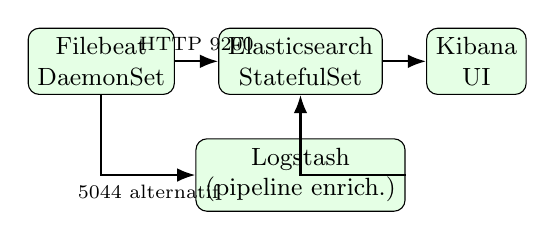
\begin{tikzpicture}[
  node distance=0.55cm and 0.55cm,
  b/.style={draw, rounded corners, fill=green!10, minimum height=0.75cm, align=center, font=\small},
  a/.style={-{Latex}, thick}
]
  \node[b] (fb) {Filebeat\\ DaemonSet};
  \node[b, right=of fb] (es) {Elasticsearch\\ StatefulSet};
  \node[b, right=of es] (kb) {Kibana\\ UI};
  \node[b, below=of es] (ls) {Logstash\\ (pipeline enrich.)};
  \draw[a] (fb) -- node[above,font=\scriptsize]{HTTP 9200} (es);
  \draw[a] (es) -- (kb);
  \draw[a] (fb.south) |- node[below,pos=.75,font=\scriptsize]{5044 alternatif} (ls.west);
  \draw[a] (ls.east) -| (es.south);
\end{tikzpicture}
\end{center}

\subsection{Elasticsearch --- stockage et recherche}
StatefulSet mono-nœud, image docker.elastic.co/elasticsearch/elasticsearch:8.14.0 :
\begin{itemize}[itemsep=1pt]
  \item discovery.type single-node, xpack.security activé (HTTP, pas TLS interne) ;
  \item heap JVM calibré : ES\_JAVA\_OPTS -Xms512m/-Xmx512m pour tenir dans la VM 4 Go ;
  \item allow\_mmap false, index buffer 64 mb, circuit breaker total 40\,\% --- réglages anti-OOM documentés ;
  \item PVC local-path 10 Gi, resources req 200m/448Mi lim 1 CPU/1024 Mi ;
  \item ELASTIC\_PASSWORD depuis Secret elasticsearch-credentials (optional:false) ;
  \item probes tcpSocket 9200 (readiness après 60 s init, liveness après 240 s) ;
  \item anti-affinité control-plane.
\end{itemize}

\subsection{Filebeat --- collecte nodale}
DaemonSet docker.elastic.co/beats/filebeat:8.14.0 :
\begin{itemize}[itemsep=1pt]
  \item autodiscovery hints Kubernetes conditionné au label part-of: devops-platform --- tout nouveau Pod de la plateforme est loggé sans config ;
  \item hostPath /var/log + /var/lib/docker/containers ;
  \item sortie directe Elasticsearch (http://elasticsearch.monitoring:9200, user elastic, worker 2) ;
  \item queue mémoire 4096 événements, flush 1024/5 s ;
  \item probe exec filebeat test config ; RBAC minimal (namespaces/nodes/pods/replicasets get-list-watch).
\end{itemize}

Note factuelle : le commentaire d'en-tête mentionne Logstash:5044 mais la configuration active sort directement vers Elasticsearch --- Logstash est déployé en parallèle, prêt à s'intercaler.

\subsection{Logstash --- pipeline de transformation}
Deployment logstash/logstash:8.14.0, stratégie Recreate, ports beats 5044 + monitoring 9600 :
\begin{lstlisting}[caption={Pipeline Logstash --- filtrage et enrichissement}]
input { beats { port => 5044 } }
filter {
  json { source => "message" target => "app" }
  mutate {
    add_field => { "service" => "%{[app][service]}"
                   "log_level" => "%{[app][level]}" }
  }
  # Drop des healthchecks : bruit pur
  if [url][path] in ["/livez", "/readyz"] { drop {} }
}
output {
  elasticsearch {
    hosts => ["http://elasticsearch.monitoring:9200"]
    user => "elastic"
    password => "${ELASTIC_PASSWORD}"
    index => "devops-platform-%{+YYYY.MM.dd}"
  }
}
\end{lstlisting}

pipeline.workers 2, batch.size 125, queue.type persisted (survit à un crash), LS\_JAVA\_OPTS 256 Mo. Credentials depuis Secret logstash-elasticsearch-auth.

\subsection{Kibana --- exploration}
Deployment kibana/kibana:8.14.0, Service 5601 :
\begin{itemize}[itemsep=1pt]
  \item auth kibana\_system + KIBANA\_PASSWORD depuis Secret dédié ;
  \item télémétrie/reporting/fleet désactivés ;
  \item NODE\_OPTIONS --max-old-space-size=320 --- dimensionnement VM ;
  \item readiness /api/status, liveness tcpSocket ; nodeSelector worker-01 + anti control-plane.
\end{itemize}

Credentials créés par \texttt{scripts/bootstrap-elasticsearch-secret.sh} : refuse les placeholders, rend le YAML dans un mktemp 0600 avec trap de nettoyage --- jamais --from-literal en argv. Post-steps imprimés : rollout restart de kibana/logstash/elasticsearch.

\begin{whybox}
ELK reste la référence open-source complète (collecte, enrichissement, plein-texte, exploration). Filebeat en DaemonSet est le pattern standard de collecte nodale ; l'autodiscovery par labels rend la couverture automatique. Toute la stack est dimensionnée au plus juste (heaps JVM réduits, queues bornées) pour tenir dans l'homelab --- contrainte réelle apprise tôt.
\end{whybox}

\subsection{Alternatives}
\begin{tabular}{@{}p{4.2cm}p{9.8cm}@{}}
\toprule
\textbf{Alternative} & \textbf{Raison du rejet} \\
\midrule
Loki + Grafana & Léger mais pas de plein-texte ni parsing riche --- objectif pédagogique ELK perdu \\
Fluentd/Fluent Bit & Solides mais Filebeat s'intègre nativement à Elastic \\
Cloud managé (ECK/Elastic Cloud) & Coût et dépendance externe \\
\bottomrule
\end{tabular}

\subsection{Captures de démonstration}
\capturebox{\texttt{kubectl get pods -n monitoring | grep -E 'elastic|filebeat|logstash|kibana'} : tous Running, DaemonSet complet.}{elk-pods-running.png}

\capturebox{Kibana Discover : index devops-platform-* sélectionné, logs JSON du service users visibles.}{kibana-discover.png}

\capturebox{Recherche Kibana filtrée : event secret.fetch ou status 503 pendant un incident Vault.}{kibana-search-vault.png}

\capturebox{Preuve drop Logstash : aucun document /livez//readyz dans l'index alors que les autres requêtes existent.}{logstash-drop-proof.png}

\capturebox{\texttt{curl -u elastic:\$PW localhost:9200/\_cat/indices} : index quotidien devops-platform-* avec docs counts.}{es-cat-indices.png}

% ------------------------------------------------------------
\section{Modèle de menaces simplifié et contre-mesures}
% ------------------------------------------------------------

Lecture croisée des outils de la plateforme sous l'angle des menaces :

\begin{longtable}{@{}p{3.6cm}p{5.6cm}p{5.0cm}@{}}
\toprule
\textbf{Menace} & \textbf{Vecteur} & \textbf{Contre-mesure(s) en place} \\
\midrule
\endhead
Secret commité & push accidentel (clé API, .env) & pre-commit gitleaks + job CI bloquant historique complet ; allowlist resserrée \\
Image vulnérable & CVE OS/lib dans l'image déployée & Trivy bloquant CRITICAL/HIGH unfixed + SBOM archivé + rescan nocturne \\
Dépendance vulnérable & requirements.txt compromis & pip-audit --strict ×4 fichiers, CI + nocturne \\
Secrets exposés au cluster & Secrets K8s lisibles / tokens longs & Vault KV-v2 TTL 1h, politiques read-only par service, NetworkPolicy 8200 seule sortie \\
Token root divulgué & argv, disque, logs & bootstrap via stdin, mktemp 0600+trap, no\_log Ansible \\
Conteneur privilégié & mauvais manifest & PSA restricted + conftest deny ×3 + Kyverno audit + securityContext strict \\
Pod root filesystem modifiable & exploitation runtime & readOnlyRootFilesystem + emptyDir /tmp \\
Mouvement latéral & Pod compromis scanne le cluster & default-deny ingress/egress + whitelist explicite \\
Dérive manuelle du cluster & kubectl edit hors process & ArgoCD selfHeal + prune \\
État Terraform corrompu & applies concurrents & backend local isolé ; contrat S3+DynamoDB prêt \\
Nœud attaqué via SSH & brute-force / root login & cloud-init : root off, passwords off, fail2ban, sudo whitelist \\
Régistre spoofé & image substituée & GHCR permissions, déploiement épinglé par digest sha256 \\
\bottomrule
\end{longtable}

\begin{whybox}
Aucun contrôle ne vaut seul : c'est la superposition (IaC durcie $\rightarrow$ images scannées $\rightarrow$ secrets dynamiques $\rightarrow$ admission restreinte $\rightarrow$ réseau fermé $\rightarrow$ GitOps auto-correctif) qui forme la défense en profondeur. Le tableau ci-dessus sert aussi de checklist d'audit : chaque ligne doit rester vraie.
\end{whybox}

\capturebox{Atelier sécurité : tentative de déploiement d'un manifest non conforme rejetée (conftest/Kyverno output).}{threatmodel-reject.png}

% ------------------------------------------------------------
\section{SLO --- objectifs de niveau de service}
% ------------------------------------------------------------

\subsection{Le contrat chiffré}
\begin{tabular}{@{}ll@{}}
\toprule
\textbf{SLI} & \textbf{SLO} \\
\midrule
Disponibilité & $\geq$ 99,9\,\% sur 30 jours \\
Latence p95 & $<$ 200 ms \\
Taux d'erreurs 5xx & $<$ 1\,\% \\
MTTD (délai de détection) & $<$ 2 min \\
MTTR (délai de rétablissement) & $<$ 30 min \\
\bottomrule
\end{tabular}

\subsection{Implémentation bout en bout}
Ces chiffres ne sont pas un slide : ils existent à trois endroits cohérents ---
\begin{enumerate}[itemsep=1pt]
  \item dans les règles Prometheus (\S AlertManager) : seuils exacts 0,1\,\% d'indispo, 0,2 s p95, 1\,\% 5xx ;
  \item dans Grafana : ligne de seuil sur le dashboard Error Rate ;
  \item dans ce rapport et la documentation plateforme.
\end{enumerate}

Les MTTD/MTTR découlent des intervalles : scrape 15 s + for 2--10 min $\Rightarrow$ détection en moins de deux minutes ; auto-réparation K8s + selfHeal ArgoCD $\Rightarrow$ rétablissement typique en secondes.

\subsection{Captures de démonstration}
\capturebox{Vue Grafana Error Rate SLO annotée : seuil 1\,\% tracé sur la courbe réelle.}{slo-grafana-threshold.png}

\capturebox{PromQL disponibilité 30 jours : \texttt{service:availability\_30d:ratio} retournant des valeurs $\approx$ 1.}{slo-recording-query.png}

\clearpage
% ============================================================
\part{Scénarios de démonstration bout en bout}
% ============================================================

Cette partie transforme les sections précédentes en \textbf{scénarios rejouables} : chaque scénario décrit l'objectif, les prérequis, les étapes exactes avec commandes, et les captures à réaliser. Ce sont ces démonstrations qui font vivre le rapport.

% ------------------------------------------------------------
\section{Scénario 1 --- Du commit au déploiement production}
% ------------------------------------------------------------

\subsection{Objectif}
Prouver la chaîne complète GitOps : un simple \texttt{git push} traverse lint, scans, build, registre, ArgoCD, jusqu'aux Pods mis à jour --- sans aucun kubectl humain.

\subsection{Prérequis}
Cluster up (validate-platform.sh vert), ArgoCD installé et Applications Synced, GHCR accessible.

\subsection{Étapes}
\begin{enumerate}[itemsep=1pt]
  \item modifier une chaîne bénigne dans \texttt{k8s/apps/users/kustomization.yaml} (ex. newTag) puis push sur secondary ;
  \item observer le run GitHub Actions déclenché par le filtre de chemins ;
  \item suivre jobs successifs : lint $\rightarrow$ gitleaks $\rightarrow$ test $\rightarrow$ build $\rightarrow$ trivy-scan ;
  \item vérifier la nouvelle image + digest dans Packages (GHCR) ;
  \item UI ArgoCD : l'Application users-service passe OutOfSync ;
  \item sync automatique : wave par wave, rollout status ;
  \item confirmer le nouveau digest côté cluster (\texttt{kubectl get deploy -o jsonpath}) ;
  \item smoke-test métriques (\texttt{/metrics} répond, séries présentes).
\end{enumerate}

\begin{lstlisting}[language=bash,caption={Commandes d'observation du scénario}]
git add -A && git commit -m "chore: bump users image" && git push
gh run watch                       # suivi du run CI
kubectl get pods -w -n devops-platform -l app=users-service
kubectl get deploy users-service \
  -o jsonpath='{.spec.template.spec.containers[0].image}'
curl -s localhost:18080/metrics | grep http_requests_total
\end{lstlisting}

\subsection{Captures du scénario}
\capturebox{Push du commit + écran Actions montrant le run démarré automatiquement.}{scenario1-01-push-run.png}

\capturebox{Chaîne des jobs au complet en vert (lint$\rightarrow$deploy-ready).}{scenario1-02-jobs-green.png}

\capturebox{GHCR : nouveau tag + digest sha256 publié.}{scenario1-03-ghcr-digest.png}

\capturebox{UI ArgoCD : carte OutOfSync avec diff affiché.}{scenario1-04-argocd-oos.png}

\capturebox{\texttt{kubectl get pods -w} : terminaison des anciens pods, création des nouveaux (rolling).}{scenario1-05-rollout.png}

\capturebox{Pod final au nouveau digest + /metrics répondant.}{scenario1-06-final-metrics.png}

% ------------------------------------------------------------
\section{Scénario 2 --- Incident Vault indisponible}
% ------------------------------------------------------------

\subsection{Objectif}
Démontrer le fail-closed de bout en bout : perte de Vault $\Rightarrow$ readiness 503 $\Rightarrow$ sortie du Service $\Rightarrow$ zéro trafic dégradé $\Rightarrow$ rétablissement propre.

\subsection{Étapes}
\begin{enumerate}[itemsep=1pt]
  \item état initial : readyz 200 pour les trois services ;
  \item simuler la panne : \texttt{kubectl scale deploy vault -n vault --replicas=0} ;
  \item observer readinessProbe échouer (périodes 5 s) puis READY 0/1 ;
  \item vérifier que le Service ne contient plus d'endpoints (curl timeout via svc) ;
  \item constater que livez reste OK : les pods ne redémarrent pas (pas de crash inutile) ;
  \item logs applicatifs : erreurs hvac structurées (vault.fetch\_failed) ;
  \item rétablir : scale --replicas=1 ; readiness repasse, endpoints reviennent ;
  \item alerte associée si prolongée : SLOAvailabilityBreach (up $<$ 99,9\,\%/30 j se dégrade progressivement).
\end{enumerate}

\begin{lstlisting}[language=bash,caption={Boîte à outils de l'incident}]
kubectl scale deploy vault -n vault --replicas=0
watch kubectl get pods -n devops-platform
kubectl get endpoints users-service -n devops-platform   # vide !
kubectl logs deploy/users-service | grep vault.fetch_failed
kubectl scale deploy vault -n vault --replicas=1          # remediation
\end{lstlisting}

\subsection{Captures du scénario}
\capturebox{Avant : readyz 200 + endpoints peuplés.}{scenario2-01-before.png}

\capturebox{Pendant : pods 0/1 READY, endpoints vide, livez toujours « alive ».}{scenario2-02-outage.png}

\capturebox{Logs JSON : événements vault.fetch\_failed horodatés.}{scenario2-03-logs.png}

\capturebox{Après : retour READY 1/1 + readyz 200.}{scenario2-04-recovery.png}

% ------------------------------------------------------------
\section{Scénario 3 --- Fuite mémoire et OOMKill}
% ------------------------------------------------------------

\subsection{Objectif}
Voir la chaîne de protection mémoire : LimitRange $\rightarrow$ limites pod $\rightarrow$ alerte 80\,\% $\rightarrow$ OOMKill $\rightarrow$ auto-réparation.

\subsection{Étapes}
\begin{enumerate}[itemsep=1pt]
  \item réduire temporairement la limite mémoire du deployment (patch kustomize overlay ou kubectl set resources) ;
  \item générer de la pression mémoire dans le pod (python boucle d'allocation) ;
  \item dashboard Infrastructure Detail : ratio monte, franchit 80\,\% ;
  \item alerte ContainerMemoryRatioHigh firing dans AlertManager ;
  \item kubelet OOMKill : Pod redémarre (RESTARTS+1), alerte PodEvictionOngoing ;
  \item restaurer les limites ; documenter en post-mortem format STAR.
\end{enumerate}

\begin{lstlisting}[language=bash,caption={Pression mémoire contrôlée}]
kubectl set resources deploy/users-service -n devops-platform \
  --limits memory=64Mi
kubectl exec deploy/users-service -- python -c "x='a'*100_000_000"
watch kubectl get pods -l app=users-service   # RESTARTS grimpe
\end{lstlisting}

\subsection{Captures du scénario}
\capturebox{Grafana : ratio mémoire franchissant 80\,\% (courbe rouge).}{scenario3-01-ratio80.png}

\capturebox{AlertManager : ContainerMemoryRatioHigh puis PodEvictionOongoing firing.}{scenario3-02-alerts.png}

\capturebox{\texttt{kubectl describe pod} : Last State: OOMKilled, exit code 137.}{scenario3-03-oomkill.png}

\capturebox{Post-mortem : timeline MTTD/MTTR mesurée depuis Grafana + Kibana.}{scenario3-04-postmortem.png}

% ------------------------------------------------------------
\section{Scénario 4 --- Stress HPA et anti-flapping}
% ------------------------------------------------------------

\subsection{Objectif}
Valider l'autoscaling asymétrique : montée rapide sous charge, descente lente et prudente.

\subsection{Étapes}
\begin{enumerate}[itemsep=1pt]
  \item baseline : HPA 2 réplicas, CPU $\approx$ 0 ;
  \item lancer stress-hpa.sh (ab -c 80 -n 4000) ;
  \item observer : cibles CPU $>$70\,\%, montée +100\,\%/30 s jusqu'à stabilisation (2$\rightarrow$5 max) ;
  \item arrêter la charge : descente bloquée pendant stabilizationWindow 300 s puis $-$25\,\%/min ;
  \item cas extrême : charge maintenue $\Rightarrow$ HPAPinnedAtMaxReplicas après 15 min.
\end{enumerate}

\subsection{Captures du scénario}
\capturebox{Watch hpa+pods pendant la montée : réplicas 2$\rightarrow$3$\rightarrow$5.}{scenario4-01-scaleup.png}

\capturebox{Grafana App Performance : RPS réparti, p95 stable malgré la charge.}{scenario4-02-perf-stable.png}

\capturebox{Descente progressive après arrêt (fenêtre 300 s visible entre deux réductions).}{scenario4-03-scaledown.png}

\capturebox{(Optionnel) HPAPinnedAtMaxReplicas firing après 15 min de charge continue.}{scenario4-04-pinned.png}

% ------------------------------------------------------------
\section{Scénario 5 --- Rollback GitOps après régression}
% ------------------------------------------------------------

\subsection{Objectif}
Montrer qu'un rollback est un revert Git : aucune manipulation cluster directe.

\subsection{Étapes}
\begin{enumerate}[itemsep=1pt]
  \item introduire volontairement une régression (endpoint /users renvoyant 500) ;
  \item push $\rightarrow$ CI verte (la CI teste la plateforme, pas la logique métier statique) $\rightarrow$ ArgoCD déploie ;
  \item constater l'erreur : dashboard Error Rate SLO franchit 1\,\%, alerte critique ;
  \item rollback : \texttt{git revert <sha>} ;
  \item ArgoCD resynchronise vers le digest précédent ; erreur disparaît ;
  \item MTTR mesuré : minutes, entièrement traçable dans l'historique.
\end{enumerate}

\begin{lstlisting}[language=bash,caption={Rollback = git revert}]
git revert --no-edit <sha-regression>
git push
# ArgoCD fait le reste; historique complet dans l'UI
\end{lstlisting}

\subsection{Captures du scénario}
\capturebox{Régression déployée : Error Rate $>$1\,\% + topk table montrant /users en tête.}{scenario5-01-error-rate.png}

\capturebox{Alerte SLO5xxErrorRateBreach critical firing.}{scenario5-02-alert.png}

\capturebox{git revert + push, ArgoCD resynchronisant le digest antérieur.}{scenario5-03-revert-sync.png}

\capturebox{Retour sous seuil : courbe Error Rate repassant sous 1\,\%.}{scenario5-04-recovered.png}

% ------------------------------------------------------------
\section{Scénario 6 --- Rotation complète des secrets}
% ------------------------------------------------------------

\subsection{Objectif}
Prouver que la rotation d'un secret critique est une opération de routine : zéro downtime visible, zéro fuite du nouveau token.

\subsection{Étapes}
\begin{enumerate}[itemsep=1pt]
  \item baseline readyz 200 ;
  \item \texttt{scripts/bootstrap-vault-secret.sh} --- génère et affiche UNE fois le token, remplace le Secret via stdin ;
  \item rotation applicative : nouvelle valeur JWT\_SECRET\_KEY dans KV ;
  \item restart rolling des deployments pour recharger les secrets au boot (modèle startup-load assumé) ;
  \item vérifier readyz 200 partout + aucun token dans l'historique shell/git.
\end{enumerate}

\begin{lstlisting}[language=bash,caption={Séquence de rotation propre}]
scripts/bootstrap-vault-secret.sh            # nouveau root token (stdin)
vault kv put secret/devops-platform/users-service \
    DATABASE_URL="..." JWT_SECRET_KEY="$(openssl rand -hex 32)"
kubectl rollout restart deploy/users-service -n devops-platform
kubectl rollout status  deploy/users-service -n devops-platform
curl -s localhost:18080/readyz               # {"vault":{"reachable":true}}
gitleaks detect --source . --no-banner       # rien dans l'historique
\end{lstlisting}

\subsection{Captures du scénario}
\capturebox{Sortie du bootstrap affichant le token une unique fois (masqué partiellement).}{scenario6-01-onetime-token.png}

\capturebox{Rolling restart : anciens/nouveaux pods coexistant brièvement (maxSurge).}{scenario6-02-rolling.png}

\capturebox{Preuves finales : readyz 200 + gitleaks clean.}{scenario6-03-proof.png}

% ------------------------------------------------------------
\section{Scénario 7 --- Détection de drift supply-chain (nocturne)}
% ------------------------------------------------------------

\subsection{Objectif}
Montrer pourquoi le cron 03h00 existe : une CVE publiée APRÈS le merge doit être détectée sans nouvelle livraison.

\subsection{Étapes}
\begin{enumerate}[itemsep=1pt]
  \item simuler l'annonce d'une CVE HIGH corrigible touchant une dépendance épinglée ;
  \item déclencher le workflow manuellement (même chaîne que le schedule 03h00) ;
  \item job test : pip-audit --strict échoue sur la dépendance ; sinon trivy attrape l'image au build suivant ;
  \item le run rouge est le signal : équipe notifiée, bump planifié ;
  \item correctif = PR classique de bump de version, repassant toute la chaîne.
\end{enumerate}

\begin{whybox}
La sécurité n'est pas un état mais un processus : ce qui était vert hier peut être rouge aujourd'hui sans qu'aucune ligne du projet ne change. Le scan nocturne transforme cette réalité en signal automatique --- c'est le MTTD de la supply chain.
\end{whybox}

\subsection{Captures du scénario}
\capturebox{Run nocturne rouge : job trivy/pip-audit en échec avec CVE listée.}{scenario7-01-nightly-red.png}

\capturebox{PR de bump : diff requirements.txt + pipeline vert après merge.}{scenario7-02-bump-pr.png}

\clearpage
% ============================================================
\part{Exploitation et synthèse}
% ============================================================

% ------------------------------------------------------------
\section{Scripts de validation de la plateforme}
% ------------------------------------------------------------

\subsection{validate-platform.sh --- les 7 contrôles}
Flags : \texttt{-{}-ci} (exit 1, outil manquant = FAIL et non SKIP), \texttt{-{}-only <ids>}, \texttt{-{}-skip-incident}, \texttt{-{}-namespace}, \texttt{-{}-image-tag}. Sorties 0/1/2.

\begin{longtable}{@{}p{0.8cm}p{5.6cm}p{7.6cm}@{}}
\toprule
\textbf{n°} & \textbf{Contrôle} & \textbf{Méthode} \\
\midrule
\endhead
1 & Cluster Kubernetes opérationnel & kubectl get nodes -o json + jq : tous Ready \\
2 & Pods en Running & readyReplicas == spec.replicas par service \\
3 & Aucune CVE critique & trivy image --severity CRITICAL,HIGH --exit-code 1 \\
4 & Aucun secret détecté & gitleaks detect --source . --config .gitleaks.toml --redact \\
5 & ArgoCD synchronisé & toutes Applications Synced + Healthy \\
6 & Dashboards Grafana actifs & deploy prêt + $\geq$3 ConfigMaps grafana\_dashboard=1 \\
7 & Logs indexés ELK & kibana prêt + ES sts prêt + filebeat complet + health green/yellow exec pod \\
Bonus A & Self-healing & delete volontaire d'un Pod users, retour attendu $<$30 s (destructif) \\
\bottomrule
\end{longtable}

\subsection{validate-security.sh --- les 4 contrôles sécurité}
Flags \texttt{-{}-ci}, \texttt{-{}-tag}, \texttt{-{}-namespace} :
\begin{enumerate}[itemsep=1pt]
  \item Gitleaks zéro secret (historique complet) ;
  \item Trivy CRITICAL/HIGH par image (exit-code 1) ;
  \item Vault initialisé ET non scellé (\texttt{vault status -format=json} exécuté dans le pod) ;
  \item preuve de vie du token root : lecture du Secret, rejet des placeholders (INJECT-VIA / DO-NOT-COMMIT), \texttt{vault token lookup} avec affichage du TTL.
\end{enumerate}

\subsection{Autres outils d'exploitation}
\begin{longtable}{@{}p{4.4cm}p{9.6cm}@{}}
\toprule
\textbf{Script} & \textbf{Rôle} \\
\midrule
\endhead
smoke-test.sh & Parcours E2E : pods prêts, endpoints via port-forward 18080--18082, targets Prometheus UP, http\_requests\_total $>$ 0, santé Grafana ; flags --ci, --skip-grafana \\
stress-hpa.sh & Charge Apache Bench -c 80 -n 4000, watch 90 s, scale 2$\rightarrow$5 attendu ; flags -c/-n/--watch/--no-watch/--ci \\
stress-panel.py & Petite UI stdlib port 8080 pilotant stress-hpa.sh : état HPA/pods/virsh/port-forward \\
generate-inventory.sh & terraform refresh + apply ciblé local\_file puis copie inventaire ; --no-refresh \\
bootstrap-vault-secret.sh & Création/rotation du Secret vault-root-token via stdin (jamais argv) ; -n/-d/--dry-run \\
bootstrap-elasticsearch-secret.sh & 3 Secrets monitoring (ES/Kibana/Logstash), mktemp 0600 + trap, refuse placeholders \\
\bottomrule
\end{longtable}

\begin{whybox}
Une plateforme non vérifiable n'existe pas : ces scripts encodent la définition de « ça marche » et servent simultanément de recette locale, de garde CI (--ci) et de démonstration. Le bonus self-healing teste le comportement --- pas la config : seule façon de prouver que l'auto-réparation fonctionne réellement.
\end{whybox}

\subsection{Captures de démonstration}
\capturebox{\texttt{scripts/validate-platform.sh} complet : les 7 contrôles + bonus en vert avec durées.}{validate-platform-all.png}

\capturebox{Mode bloquant : \texttt{-{}-ci} sur une plateforme volontairement cassée (pod scaled down) --- exit code 1 visible.}{validate-platform-fail.png}

\capturebox{Bonus self-healing en direct : delete du pod puis retour Ready en $<$30 s dans la sortie du script.}{validate-selfheal.gif}

\capturebox{\texttt{scripts/validate-security.sh} : 4 contrôles verts dont le TTL du token Vault affiché.}{validate-security-ok.png}

\capturebox{\texttt{scripts/smoke-test.sh} : parcours E2E complet vert.}{smoke-e2e.png}

% ------------------------------------------------------------
\section{Tests de charge --- HPA en conditions réelles}
% ------------------------------------------------------------

\subsection{Apache Bench via stress-hpa.sh}
Charge immédiate sans dépendance : \texttt{ab -c 80 -n 4000} contre users-service, watch 90 s. Résultat attendu : HPA monte de 2 à 5 réplicas (CPU cible 70\,\% dépassée), vérifié par --ci.

\subsection{k6 --- test scripté nocturne (à écrire)}
Le job GitHub Actions load-test appelle \texttt{tests/k6/load-test.js} (grafana/k6-action@v0.3.1, BASE\_URL configurable) : scénarios JS versionnés, seuils pass/fail, résultats JSON archivés 14 jours. \textbf{Le fichier n'existe pas encore} --- première action corrective du projet.

\begin{whybox}
Deux niveaux complémentaires : ab répond à « est-ce que ça scale maintenant » pendant une session interactive ; k6 permet des scénarios reproductibles versionnés (rampe, paliers, seuils SLO) rejoués automatiquement chaque nuit --- détection de régressions de performance avant la production.
\end{whybox}

\subsection{Captures de démonstration}
\capturebox{\texttt{watch kubectl get hpa,pods} pendant stress-hpa.sh : réplicas montant 2$\rightarrow$5 en temps réel.}{hpa-scaling-live.png}

\capturebox{Sortie ab : RPS, latences percentiles sous charge.}{ab-results.png}

\capturebox{Grafana pendant le test : RPS et p95 montent, réplicas suivent (dashboard App Performance).}{grafana-under-load.png}

\clearpage
% ------------------------------------------------------------
\section{Index des runbooks}
% ------------------------------------------------------------

Procédures d'urgence condensées (détail : scénarios et scripts associés) :

\begin{longtable}{@{}p{4.2cm}p{6.6cm}p{3.4cm}@{}}
\toprule
\textbf{Symptôme} & \textbf{Premiers réflexes} & \textbf{Outils} \\
\midrule
\endhead
Pod CrashLoopBackOff & logs + describe (exit code), vérifier secrets Vault & kubectl, Kibana \\
Vault scellé/indispo & vault status ; readiness 503 assumé ; ne pas forcer les pods & vault CLI, AM alertes \\
OOMKill récurrent & ratio mémoire Grafana, remonter limites via overlay & KSM, rules.yaml \\
HPA bloqué au max & chercher fuite mémoire ; incident 9 post-mortem & stress-panel.py \\
Dérive cluster vs Git & UI ArgoCD diff ; ne jamais fixer à la main & ArgoCD selfHeal \\
5xx en hausse & dashboard Error Rate $\rightarrow$ handler fautif $\rightarrow$ logs filtrés & Grafana+Kibana \\
Image non tirée & digest présent GHCR ? netpol egress DNS ? & crictl, netpol \\
Cluster injoignable & virsh list ; systemd kubelet/containerd sur nœud & libvirt, journalctl \\
Secret expiré (401 Vault) & rotation bootstrap-vault-secret.sh puis rollout & script + ArgoCD sync \\
Disque ES plein & retention/ILM, taille PVC 10Gi, purger indices vieux & \_cat/indices \\
\bottomrule
\end{longtable}

% ------------------------------------------------------------
\section{Tableau récapitulatif général}\label{sec:recap}
% ------------------------------------------------------------

{\footnotesize
\begin{longtable}{@{}p{3.0cm}p{1.9cm}p{4.7cm}p{4.7cm}@{}}
\caption{Toutes les technologies du projet : version, rôle, raison du choix}\\
\toprule
\textbf{Outil} & \textbf{Version} & \textbf{Ce qu'il fait ici} & \textbf{Pourquoi lui} \\
\midrule
\endfirsthead
\toprule
\textbf{Outil} & \textbf{Version} & \textbf{Ce qu'il fait ici} & \textbf{Pourquoi lui} \\
\midrule
\endhead
Libvirt/KVM & QEMU-KVM & 3 VMs q35 virtio, réseau NAT dédié & VMs réalistes gratuites, reproductibles \\
cloud-init & Ubuntu 22.04 img & Provisionnement + durcissement boot & Standard first-boot, durcit avant tout \\
Terraform & $\sim$1.5 (CI 1.5.7) & IaC réseau, volumes, VMs, inventaire & Standard IaC, plan/état/dérive \\
Provider libvirt & 0.9.8 & Piloter KVM depuis Terraform & Seul provider KVM mature \\
hashicorp/local & 2.9.0 & Rendre le fichier inventaire & Artefacts locaux idempotents \\
Ansible & collection 8.0.0 & Config Docker, K8s, jointure, CNI & Agentless, idempotent, lisible \\
Docker CE & repo officiel & Builds multi-stage des images & Référence construction OCI \\
containerd & repo officiel & Runtime CRI des Pods & Recommandé kubeadm, léger \\
Kubernetes & 1.28 (held) & Orchestration, autoscaling, auto-rép & API universelle orchestration \\
kubeadm & 1.28 & Cycle de vie cluster & Officiel, conforme upstream \\
Calico & v3.26.1 Tigera & CNI routage + NetworkPolicies & Mature, ingress+egress complets \\
Kustomize & 5.4.3 & Base + overlays env & Patch sans template, natif GitOps \\
FastAPI & 0.139.0 & Framework HTTP services & Pydantic, OpenAPI, async \\
Uvicorn & $\geq$0.24 std & Serveur ASGI port 8000 & Référence ASGI \\
hvac & 2.1.0 & Client Vault KV-v2 & Client Python de référence \\
python-json-logger & 2.0.7 & Logs JSON stdout & Structuré ELK, minimal \\
prometheus-fastapi-instrumentator & 6.1.0 & Métriques RED /metrics & Une ligne = histogramme normalisé \\
Vault & 1.15.2 dev mode & Secrets dynamiques, auth K8s TTL 1h & Rotation/révocation centralisée \\
GitHub Actions & --- & Pipeline CI/CD + jobs nocturnes & CI native dépôt, matrice, OIDC \\
GHCR & ghcr.io & Registre images & Colocalisé, permissions héritées \\
Gitleaks & 8.18.0 & Détection secrets local+CI & Scan historique rapide, config maison \\
Trivy & action v0.24.0 & Scan CVE bloquant, SARIF, SBOM & Scanner unifié CNCF \\
pip-audit & --strict & Audit requirements Python & Officiel PyPA \\
Ruff & 0.1.9 & Linter Python & Ultra-rapide, remplace 3 outils \\
yamllint & 1.33.0 & Hygiène YAML & Simple, pre-commit+CI \\
kubeconform & 0.6.4 & Validation schémas K8s 1.28 & Hors ligne, rapide \\
conftest (Rego) & mode audit & Politiques sécurité manifests & Policy-as-code pré-admission \\
Kyverno & Audit & Policies admission cluster & Natif K8s, audit$\rightarrow$enforce \\
pre-commit & 11 hooks & Qualité avant push (5 dépôts) & Shift-left, parité CI \\
ArgoCD & v2.7.16 & GitOps pull, prune, selfHeal, waves & État cluster = Git, rollback = revert \\
Prometheus Operator & v0.74.0 & CRDs ServiceMonitor/PrometheusRule & Découverte déclarative GitOps \\
Prometheus & v2.51.0 & Collecte 15 s, rétention 15 j & Standard métriques, PromQL \\
kube-state-metrics & v2.10.1 & État objets en métriques & Source alertes HPA/OOM \\
AlertManager & v0.27.0 & Groupement/routage alertes & Routage standard écosystème \\
Grafana & 11.1.0 & Dashboards provisionnés sidecar & Dashboards-as-code versionnés \\
kiwigrid sidecar & 1.27.6 & Chargement dashboards ConfigMap & Provisionnement auto \\
Elasticsearch & 8.14.0 & Stockage/recherche logs & Plein-texte, référence ELK \\
Filebeat & 8.14.0 DaemonSet & Collecte logs nœuds/Pods & Autodiscovery K8s standard \\
Logstash & 8.14.0 & Enrichissement, drop healthchecks & Transformation events \\
Kibana & 8.14.0 & Exploration logs & UI recherche standard ELK \\
Apache Bench & ab -c80 -n4000 & Génération charge HPA & Zéro dépendance \\
k6 & action v0.3.1 & Test charge scripté nocturne & Scénarios JS versionnés (à écrire) \\
jq/curl & --- & Manipulation JSON scripts & Bases scripting exploitation \\
\bottomrule
\end{longtable}
}

\clearpage
% ------------------------------------------------------------
\section{Limites connues et axes d'amélioration}
% ------------------------------------------------------------

Lecture honnête du code actuel :
\begin{itemize}[itemsep=2pt]
  \item \texttt{tests/k6/load-test.js} n'existe pas : le job nocturne échoue systématiquement --- priorité n°1 ;
  \item job deploy lit needs.build.outputs.image (une chaîne pour 3 lignes de matrice : dernière gagnante) --- limitation documentée inline ;
  \item trivy-scan résout les images par tag github.ref\_name et non par digest malgré l'intention affichée ;
  \item Vault reste en dev mode (in-memory, auto-unseal, token root partagé) : raft/TLS/injector préparés mais non câblés côté Pods ;
  \item overlay dev patche réplicas à 1 sans retirer les HPA (min 2) : conflit latent ;
  \item AppProject ArgoCD conserve destinations istio-system/flagger-system héritées de la stack canary supprimée ;
  \item Filebeat commenté comme envoyant vers Logstash:5044 alors qu'il écrit directement Elasticsearch ;
  \item corruption cosmétique d'accents dans quelques chaînes de validate-platform.sh (logique intacte) ;
  \item checksum manifest Tigera non vérifié (TODO inline) ; host\_key\_checking=False assumé lab.
\end{itemize}

Chaque point est borné et actionnable --- aucun ne compromet l'architecture d'ensemble ; plusieurs sont déjà documentés inline dans le code concerné.

% ------------------------------------------------------------
\section{Conclusion}
% ------------------------------------------------------------

DevOps Central Platform démontre qu'une chaîne DevOps professionnelle complète peut tenir dans un homelab : Terraform provisionne, cloud-init durcit, Ansible installe, Docker empaquette, Kubernetes orchestre, GitHub Actions vérifie et pousse, Trivy/Gitleaks/pip-audit filtrent la supply chain, Vault distribue les secrets en fail-closed, ArgoCD maintient Git comme unique source de vérité, Prometheus/Grafana/ELK rendent le tout observable et les SLO le rendent contractuel.

Trois enseignements traversent ce rapport :

\begin{enumerate}[itemsep=2pt]
  \item \textbf{Chaque outil a été choisi pour une raison précise}, opposable aux alternatives --- et cette justification est documentée outil par outil dans les encadrés dédiés ;
  \item \textbf{La sécurité est transversale, pas additive} : elle apparaît au boot (cloud-init), dans les manifests (PSA, netpol, securityContext), dans la CI (scans bloquants), dans l'applicatif (fail-closed) et à l'admission (Kyverno) ;
  \item \textbf{L'honnêteté technique fait partie du design} : les limites sont listées, les incidents ont leurs alertes, les TODO sont inline. C'est cette double visibilité (ce qui marche, ce qui manque, pourquoi) qui distingue un exercice d'ingénierie d'un assemblage de tutoriels.
\end{enumerate}

\clearpage
% ============================================================
\part*{Annexes}
% ============================================================
\addcontentsline{toc}{part}{Annexes}

% ------------------------------------------------------------
\section*{Annexe A --- Commandes utiles}
\addcontentsline{toc}{section}{Annexe A --- Commandes utiles}

\begin{lstlisting}[language=bash,caption={Aide-mémoire d'exploitation quotidienne}]
# Cycle infra
cd terraform && terraform init && terraform apply
scripts/generate-inventory.sh            # ou --no-refresh
cd ../ansible && ansible-playbook playbook.yml

# Deploiement cluster
kubectl apply -f k8s/apps/base/namespace.yaml
kubectl apply -f k8s/vault/manifests.yaml
scripts/bootstrap-vault-secret.sh
kubectl apply -f k8s/apps/
kubectl apply -k k8s/argocd/install/

# Validation
scripts/validate-platform.sh             # resume
scripts/validate-platform.sh --ci        # bloquant
scripts/validate-platform.sh --skip-incident
scripts/validate-security.sh

# Tests locaux
ENVIRONMENT=dev LOG_FORMAT=plain VAULT_ADDR="" pytest -q tests/ -v
ruff check app/

# Builds images
for svc in users-service products-service orders-service; do
  docker build -t "${svc}:1.0.0" -f "app/${svc}/Dockerfile" app/
done

# Charge / HPA
scripts/stress-hpa.sh --watch 90
\end{lstlisting}

% ------------------------------------------------------------
\section*{Annexe B --- Variables d'environnement}
\addcontentsline{toc}{section}{Annexe B --- Variables d'environnement}

\begin{longtable}{@{}p{4.9cm}p{3.5cm}p{5.6cm}@{}}
\toprule
\textbf{Variable} & \textbf{Défaut (.env.example)} & \textbf{Rôle} \\
\midrule
\endhead
ENVIRONMENT & dev & active replis dev (sqlite mémoire, token éphémère) \\
SERVICE\_NAME & users-service & construit le chemin Vault par service \\
LOG\_LEVEL & DEBUG & verbosité logging \\
LOG\_FORMAT & plain & json (prod) | plain (dev) \\
VAULT\_ADDR & http://localhost:8200 & adresse API Vault \\
VAULT\_TOKEN & (vide) & token direct (dev) ; alias VAULT\_DEV\_\newline ROOT\_TOKEN\_ID \\
DATABASE\_URL & vide & secret par service \\
JWT\_SECRET\_KEY & vide & users-service \\
API\_KEY & vide & products-service \\
PAYMENT\_GATEWAY\_\newline KEY & vide & orders-service \\
\bottomrule
\end{longtable}

% ------------------------------------------------------------
\section*{Annexe C --- Index des captures demandées}
\addcontentsline{toc}{section}{Annexe C --- Index des captures demandées}

Liste de contrôle des principaux fichiers attendus dans \texttt{images/} --- les cadres numérotés du corps du rapport font foi et contiennent chacun la description exacte (161 emplacements au total, scénarios 1--7 compris) :

{\footnotesize
\begin{longtable}{@{}p{5.6cm}p{9.4cm}@{}}
\toprule
\textbf{Fichier} & \textbf{Contenu à capturer} \\
\midrule
\endhead
architecture-globale.png & Schéma global VMs/cluster/namespaces/flux \\
reseau-libvirt.png & virsh net-dumpxml / vue réseau virt-manager \\
vms-topologie.png & virsh list + dominfo des 3 nœuds \\
ip-statique-dns.png & ip addr + ping inter-nœuds depuis master \\
exemple-emplacement.png & (capture d'exemple, remplaçable) \\
kvm-virsh-list.png & virsh list --all + dumpxml memory/vcpu \\
kvm-console-boot.png & Console VNC au boot Ubuntu 22.04 \\
kvm-qcow2-info.png & qemu-img info base + volume nœud \\
cloudinit-userdata.txt.png & user-data rendu dans /var/lib/cloud \\
cloudinit-userdata.png & idem nommage principal \\
cloudinit-ssh-hardening.png & ssh root refusé vs devops accepté \\
cloudinit-fail2ban.png & fail2ban-client status sshd \\
terraform-init.png & init providers 0.9.8 / 2.9.0 \\
terraform-plan.png & plan create N ressources \\
terraform-state-list.png & terraform state list \\
terraform-outputs.png & outputs master/worker ips \\
terraform-tfstate-gitignore.png & git status sans tfstate \\
terraform-inventory-gen.png & generate-inventory.sh + inventory.ini \\
ansible-playbook-start.png & list-tasks / début run \\
ansible-recap.png & PLAY RECAP vert \\
ansible-dpkg-hold.png & apt-mark showhold \\
ansible-nodes-ready.png & get nodes après run \\
ansible-join-perms.png & ls -l /tmp/kubeadm-join* \\
ansible-calico-running.png & pods calico-system Running \\
docker-build.png & build multi-stage \\
docker-images-sizes.png & docker images/history tailles \\
docker-inspect-user-health.png & User appuser + Healthcheck \\
docker-run-healthy.png & docker ps healthy \\
containerd-crictl-ps.png & crictl ps sur un nœud \\
containerd-systemdcgroup.png & grep SystemdCgroup config.toml \\
containerd-status.png & systemctl status containerd \\
k8s-clusterinfo.png & cluster-info + version \\
k8s-controlplane-pods.png & pods kube-system sains \\
k8s-nodes-wide.png & get nodes -o wide IPs/containerd \\
k8s-calico-connectivity.png & ping/DNS inter-Pods inter-nœuds \\
kustomize-prod-render.png & kustomize build prod (replicas 3, digests) \\
k8s-limitrange-quota.png & describe limitrange + resourcequota \\
k8s-netpol-list.png & get networkpolicy (6) \\
k8s-netpol-deny-proof.png & flux refusé vs autorisé \\
k8s-hpa-status.png & get hpa targets/réplicas \\
k8s-pdb.png & get pdb allowed disruptions \\
k8s-rolling-update.png & rollout watch maxSurge/maxUnavailable \\
k8s-securitycontext.png & describe pod security context \\
fastapi-swagger.png & /docs Swagger UI \\
fastapi-root.png & JSON racine vault\_configured:true \\
fastapi-readyz-vault.png & readyz 200 vs 503 \\
fastapi-failclosed-crash.png & CrashLoop + SystemExit logs \\
shared-logs-json.png & logs JSON event secret.fetch \\
shared-logs-plain-dev.png & format plain + warning default\_used \\
shared-fail-closed-local.png & SystemExit local sans VAULT\_ADDR \\
instrumentator-metrics.png & curl /metrics histogramme \\
instrumentator-grafana-app.png & dashboard perf alimenté \\
vault-status.png & pods + vault status unsealed \\
vault-mounts-auth.png & secrets list + auth list \\
vault-policy-read.png & policy read least-privilege \\
vault-kv-get.png & kv get users-service clés \\
vault-token-rotation.png & bootstrap rotation one-shot \\
vault-readyz-after-rotation.png & readyz 200 post-rotation \\
ci-actions-list.png & runs récents statuts/durées \\
ci-graph.png & graphe jobs du run \\
ci-lint-job.png & étapes lint vertes \\
ci-test-pipaudit.png & pip-audit x4 + pytest \\
ci-build-matrix.png & matrice 3 builds tags \\
ci-trivy-pass.png & table vide + SARIF upload \\
ci-security-tab.png & Code scanning alerts \\
ci-ghcr-packages.png & packages tags branche/sha/latest \\
ci-deploy-manual.png & dispatch production + deploy complet \\
gitleaks-clean.png & detect exit 0 \\
gitleaks-detection.png & faux token détecté (contrôlé) \\
gitleaks-ci-job.png & job CI vert \\
trivy-scan-local.png & tableau CVE image \\
trivy-blocked.png & --exit-code 1 code retour 1 \\
trivy-sbom.png & artefact SPDX aperçu \\
pipaudit-clean.png & audit strict clean \\
pipaudit-detection.png & CVE Flask simulées \\
precommit-allfiles.png & 11 hooks Passed \\
precommit-fix.png & hook corrigeant + re-stage \\
conftest-pass.png & conftest sur manifests conformes \\
conftest-deny.png & 3 deny messages contrôlés \\
kyverno-policies.png & get clusterpolicy Audit \\
ruff-clean.png & ruff check All checks passed \\
kubeconform-valid.png & find+kubeconform reproduisant CI \\
argocd-apps-grid.png & tuiles 12 Applications Synced \\
argocd-app-detail.png & arbre ressources + digest + historique \\
argocd-selfheal.png & scale manuel corrigé auto \\
argocd-prune.png & ressource supprimée par prune \\
argocd-rollback.png & rollback UI diff \\
prom-operator-cr.png & get prometheus READY \\
prom-targets-up.png & Targets tous UP \\
prom-promql-rps.png & graph rate(http\_requests\_total) \\
prom-servicemonitors.png & get servicemonitor liste \\
ksm-metrics.png & kube\_hpa séries via port-forward \\
kubelet-scrape-targets.png & targets cadvisor 3 IP \\
am-ui-groups.png & alertes groupées/silences \\
am-rule-in-cluster.png & prometheusrule sync \\
am-hpa-firing.png & HPAPinnedAtMaxReplicas firing \\
am-slo-breach.png & 5xx seuil + alerte \\
grafana-infra-overview.png & dashboard Infrastructure Overview \\
grafana-app-perf.png & RPS + p95/p99 en charge \\
grafana-error-rate.png & seuil 1\,\% visible \\
grafana-infra-detail-oom.png & ratio rouge + OOMKill \\
grafana-dash-configmaps.png & 4 ConfigMaps labellisés \\
elk-pods-running.png & ES/filebeat/logstash/kibana Running \\
kibana-discover.png & index devops-platform-* logs JSON \\
kibana-search-vault.png & filtre event secret.fetch / 503 \\
logstash-drop-proof.png & absence documents livez/readyz \\
es-cat-indices.png & indices quotidiens docs counts \\
slo-grafana-threshold.png & seuil SLO tracé \\
slo-recording-query.png & availability\_30d ratio \\
validate-platform-all.png & 7 contrôles + bonus verts \\
validate-platform-fail.png & --ci exit 1 contrôlé \\
validate-selfheal.gif & delete pod + retour $<$30 s \\
validate-security-ok.png & 4 contrôles + TTL token \\
smoke-e2e.png & smoke-test complet vert \\
hpa-scaling-live.png & watch hpa/pods 2$\rightarrow$5 \\
ab-results.png & RPS + percentiles ab \\
grafana-under-load.png & dashboards pendant charge \\
\bottomrule
\end{longtable}
}

\vspace{4mm}
\begin{center}
\rule{0.4\linewidth}{0.4pt}\\[3mm]
Fin du rapport.
\end{center}

% ------------------------------------------------------------
\section*{Annexe D --- Arborescence commentée du dépôt}
\addcontentsline{toc}{section}{Annexe D --- Arborescence commentée}

\begin{lstlisting}[caption={Structure complete du projet (fichiers cles)}]
devops-central-platform/
|-- .github/workflows/ci-cd.yml     # pipeline complet (447 lignes)
|-- .gitleaks.toml                  # config scan secrets (allowlist serree)
|-- .pre-commit-config.yaml         # 11 hooks / 5 depots
|-- .dockerignore                   # contexte build minimal
|-- .env.example                    # variables documentees
|
|-- terraform/
|   |-- main.tf                     # reseau, volumes, VMs, inventaire
|   |-- variables.tf                # 12 variables validees
|   |-- outputs.tf                  # ips sensibles, inventaire
|   |-- backend.tf                  # local actif; contrat S3+DynamoDB commente
|   |-- cloud-init.tpl              # durcissement boot
|   `-- inventory.tpl               # rendu [masters]/[workers]
|
|-- ansible/
|   |-- ansible.cfg                 # forks=10, pipelining
|   |-- playbook.yml                # 5 plays (dont reset double opt-in)
|   |-- requirements.yml            # community.general==8.0.0
|   |-- group_vars/all.yml          # k8s 1.28, calico v3.26.1, CIDRs
|   `-- roles/{docker,k8s_common,k8s_master,k8s_worker,k8s_reset}/
|
|-- app/
|   |-- users-service/              # main.py + Dockerfile + requirements.txt
|   |-- products-service/
|   |-- orders-service/
|   `-- shared/                     # vault_client.py, log_config.py,
|                                   # config.py, pyproject.toml
|
|-- k8s/
|   |-- apps/                       # base/ + users/products/orders + overlays
|   |-- monitoring/
|   |   |-- base/                   # ns monitoring + quota + limitrange
|   |   |-- prometheus/             # operator 0.74 + prom v2.51 (+helm alt.)
|   |   |-- alertmanager/           # am v0.27 + rules.yaml (SLO)
|   |   |-- grafana/                # 11.1 + sidecar + 4 dashboards CM
|   |   |-- elk/                    # es/filebeat/logstash/kibana 8.14
|   |   |-- kubelet/                # scrape cadvisor explicite
|   |   `-- kube-state-metrics/     # v2.10.1
|   |-- argocd/{install/,applications/}  # v2.7.16 + AppProject + 12 Apps
|   |-- vault/                      # manifests dev-mode + policy.hcl
|   `-- policies/                   # conftest rego + kyverno audit
|
|-- scripts/
|   |-- validate-platform.sh        # 7 controles + self-heal
|   |-- validate-security.sh        # 4 controles securite
|   |-- generate-inventory.sh       # terraform -> ansible
|   |-- bootstrap-vault-secret.sh   # rotation stdin
|   |-- bootstrap-elasticsearch-secret.sh
|   |-- smoke-test.sh / stress-hpa.sh / stress-panel.py
|
`-- tests/test_services.py          # pytest (ENVIRONMENT=dev)
\end{lstlisting}

% ------------------------------------------------------------
\section*{Annexe E --- Glossaire}
\addcontentsline{toc}{section}{Annexe E --- Glossaire}

\begin{description}[itemsep=2pt,leftmargin=1.6em]
  \item[ASGI] Interface serveur-application asynchrone de Python (successeur de WSGI) --- Uvicorn l'implémente, FastAPI s'y appuie.
  \item[ArgoCD] Contrôleur GitOps : synchronise en continu le cluster avec les manifests d'un dépôt Git.
  \item[CIDR] Notation d'un bloc d'adresses IP (ex. 192.168.0.0/16).
  \item[CNI] Container Network Interface --- plugin réseau des Pods ; Calico ici.
  \item[CRI] Container Runtime Interface --- API entre kubelet et runtime ; containerd ici.
  \item[DaemonSet] Objet K8s exécutant un Pod sur chaque nœud (Filebeat, calico-node).
  \item[DevSecOps] Intégration de la sécurité dans chaque étape du cycle DevOps.
  \item[Digest] Empreinte immuable sha256 d'une image OCI.
  \item[fail-closed] Politique refusant tout fonctionnement dégradé silencieux : sans secret résolvable, on refuse de démarrer.
  \item[GitOps] Modèle opérationnel où Git est la source de vérité de l'état du système ; le cluster tire et réconcilie.
  \item[HEALTHCHECK] Instruction Docker exécutant périodiquement un test de santé embarqué à l'image.
  \item[Helm/Kustomize] Deux approches du packaging Kubernetes : templates paramétrables vs patches sur YAML concret.
  \item[HPA] Horizontal Pod Autoscaler --- ajuste le nombre de réplicas selon CPU/mémoire.
  \item[IaC] Infrastructure as Code --- infrastructure décrite en code versionné (Terraform).
  \item[KV-v2] Moteur de secrets Vault avec historique de versions et soft-delete.
  \item[liveness/readiness/startup] Les trois probes Kubernetes : vivant / prêt à servir / grâce au démarrage.
  \item[MTTD/MTTR] Mean Time To Detect / To Recover --- délais de détection et de rétablissement.
  \item[NetworkPolicy] Pare-feu L3/L4 déclaratif entre Pods (Calico l'applique).
  \item[OOMKill] Destruction d'un conteneur par le kernel lorsque sa limite mémoire est atteinte.
  \item[PDB] PodDisruptionBudget --- garantit un minimum de réplicas pendant les perturbations volontaires.
  \item[PromQL] Langage de requête des séries temporelles Prometheus.
  \item[PSA restricted] Profil Pod Security Admission le plus strict : pas de root, caps limitées, seccomp obligatoire...
  \item[Recording rule] Règle Prometheus pré-calculant une expression coûteuse en une nouvelle série.
  \item[SBOM] Software Bill of Materials --- inventaire normalisé des composants d'une image (SPDX ici).
  \item[ServiceMonitor] CRD du Prometheus Operator déclarant une cible de scraping.
  \item[SLO/SLI] Service Level Objective / Indicator --- objectifs mesurés par indicateurs (99,9\,\%, p95...).
  \item[sync waves] Ordonnancement ArgoCD : les ressources de wave N attendent la santé des waves précédentes.
  \item[taint/toleration, affinity] Mécanismes de placement des Pods sur les nœuds.
\end{description}

% ------------------------------------------------------------
\section*{Annexe F --- Journal des décisions (extraits ADR)}
\addcontentsline{toc}{section}{Annexe F --- Journal des décisions}

Format court : Décision $\rightarrow$ Contexte $\rightarrow$ Conséquence.

\begin{longtable}{@{}p{4.2cm}p{5.6cm}p{4.2cm}@{}}
\toprule
\textbf{Décision} & \textbf{Contexte} & \textbf{Conséquence} \\
\midrule
\endhead
Terraform épinglé \textasciitilde1.5 & Éviter ruptures 1.6+ & CI rejoue exactement 1.5.7 ; migration OpenTofu différée \\
4096 Mo par nœud & kubelet NodeStatusUnknown à 2 Go sous ELK+ArgoCD & Homelab plus gourmand mais stable \\
Inventaire généré par Terraform & Inventaires manuels divergent toujours & zéro édition main ; --no-refresh disponible \\
Addons kubeadm différés & CoreDNS CrashLoop sans CNI & init en deux phases dans Ansible \\
Calico fail-closed & Un CNI cassé = cluster mort & attente Ready bloquante, abort assumé \\
dpkg hold kubelet, kubeadm, kubectl & apt upgrade casse le pin 1.28 & holds posés par Ansible \\
no\_log sur join command & token bootstrap dans logs CI & fichiers 0600 sur master \\
Secrets fail-closed applicatifs & JWT signable avec clé dev = fuite & SystemExit au démarrage prod \\
Deploy manuel uniquement & Prod jamais poussée automatiquement & workflow\_dispatch + environnement GitHub \\
Tags images branche+sha & :latest mutable = rollback impossible & latest réservé branche par défaut \\
Trivy bloquant CRITICAL/HIGH unfixed & Pipeline vivant malgré faux positifs & SARIF pour le suivi, SBOM archivé \\
conftest/Kyverno en Audit & Mesurer le bruit avant bloquer & passage enforce prévu après stabilisation \\
Vault dev mode assumé & Lab homelab, TLS/raft lourds & chemin production documenté, injector prêt \\
GitOps pull (ArgoCD) & CI push = credentials cluster côté SaaS & selfHeal + prune + revert = rollback \\
\bottomrule
\end{longtable}

% ------------------------------------------------------------
\section*{Annexe G --- Cartographie des ports et endpoints}
\addcontentsline{toc}{section}{Annexe G --- Ports et endpoints}

\begin{longtable}{@{}p{4.6cm}p{2.2cm}p{7.2cm}@{}}
\toprule
\textbf{Composant} & \textbf{Port} & \textbf{Usage} \\
\midrule
\endhead
Microservices (3×) & 8000 & HTTP app + /metrics + probes \\
Services K8s apps & 80 & ClusterIP vers 8000 \\
Vault & 8200 & API KV/auth \\
Vault metrics & 8201 & /v1/sys/metrics \\
Prometheus & 9090 & UI + TSDB \\
AlertManager & 9093 & UI + API alertes \\
Grafana & 3000 & UI dashboards \\
Elasticsearch & 9200 / 9300 & HTTP / transport \\
Logstash beats & 5044 & entrée Beats (réserve) \\
Logstash monitor & 9600 & API node stats \\
Kibana & 5601 & UI exploration \\
kubelet metrics & 10250 & https-metrics/cadvisor \\
SSH nœuds & 22 & clés uniquement (durci) \\
Endpoints HTTP app & --- & / · /livez · /readyz · /metrics · /users·/products·/orders \\
\bottomrule
\end{longtable}

% ------------------------------------------------------------
\section*{Annexe H --- Checklists d'exploitation}
\addcontentsline{toc}{section}{Annexe H --- Checklists d'exploitation}

\subsection*{Quotidienne (5 min)}
\begin{enumerate}[itemsep=1pt]
  \item run nocturne CI vert ? (sinon : CVE/drift $\rightarrow$ Annexe runbooks)
  \item \texttt{kubectl get pods -A | grep -v Running} : vide ?
  \item UI ArgoCD : toutes Applications Synced/Healthy ?
  \item Grafana Error Rate SLO $<$1\,\% et p95 $<$200 ms sur 24 h ?
  \item AlertManager : aucun firing non acquitté ?
\end{enumerate}

\subsection*{Hebdomadaire (20 min)}
\begin{enumerate}[itemsep=1pt]
  \item \texttt{scripts/validate-platform.sh} complet avec bonus self-heal ;
  \item \texttt{scripts/validate-security.sh} : TTL token Vault vérifié ;
  \item Prometheus targets : zéro down depuis 7 jours ;
  \item Elasticsearch : taille indices, rétention 15 j respectée ;
  \item GHCR : purger les tags de branches supprimées ;
  \item revue des silences AlertManager créés (à lever si obsolètes).
\end{enumerate}

\subsection*{Mensuelle (1 h)}
\begin{enumerate}[itemsep=1pt]
  \item rotation du token root Vault + preuve validate-security ;
  \item rotation JWT\_SECRET\_KEY/API\_KEY/PAYMENT\_GATEWAY\_KEY ;
  \item mise à jour mineure des dépendances (PR bump + chaîne complète) ;
  \item test restore : recréation VM via Terraform destroy/create sur worker de test ;
  \item revue des quotas ResourceQuota vs consommation réelle ;
  \item relecture du tableau menaces/contre-mesures (chaque ligne encore vraie ?).
\end{enumerate}

\capturebox{Checklist hebdo exécutée en terminal : validate-platform 7+bonus verts.}{checklist-weekly.png}

% ------------------------------------------------------------
\section*{Annexe I --- Banque de questions / réponses éclair}
\addcontentsline{toc}{section}{Annexe I --- Questions et réponses éclair}

Alignée sur l'objectif du projet (raconter les choix au format STAR en entretien).

\begin{longtable}{@{}p{6.2cm}p{8.0cm}@{}}
\toprule
\textbf{Question} & \textbf{Réponse éclair} \\
\midrule
\endhead
Pourquoi Terraform plutôt que Ansible pour créer les VMs ? & Gestion d'état + plan/prévisualisation ; Ansible est idempotent mais sans état : la dérive serait invisible. Les deux se complètent (provision vs configure). \\
Pourquoi containerd et pas Docker runtime ? & Depuis 1.24, dockershim supprimé ; containerd = CRI natif, surface réduite, chemin industriel. Docker reste pour le build. \\
SystemdCgroup, pourquoi c'est vital ? & kubelet et runtime doivent partager le même driver cgroup sinon OOMKills fantômes et évictions injustifiées. \\
Pourquoi différer CoreDNS/kube-proxy après Calico ? & Sans CNI, ces addons CrashLoop ; init en deux phases = bootstrap déterministe. \\
Pourquoi Calico vs Flannel ? & NetworkPolicy ingress+egress complète --- le modèle default-deny du projet en dépend. \\
Kustomize ou Helm pour vos apps ? & Kustomize : patch sans template, diffs Git lisibles, natif ArgoCD. Helm gardé pour stacks tierces paramétrables. \\
readiness vs liveness ici ? & livez = processus vivant (aucune dépendance) ; readyz = Vault joignable. Séparation = pas de crash inutile, mais sortie propre du Service. \\
Que se passe-t-il si Vault tombe ? & readyz 503 $\rightarrow$ endpoints vidés $\rightarrow$ zéro trafic servi dégradé. livez OK donc pas de redémarrage inutile. Rétablissement = retour automatique. \\
Fail-closed, pourquoi refuser de démarrer ? & Un fallback silencieux signerait des JWT avec une clé prévisible --- pire que l'indisponibilité. \\
Pourquoi un token root hors bande ? & Jamais en argv (ps), disque (mktemp 0600), ni Git (gitleaks) ; stdin only, affiché une fois. \\
Comment garantissez-vous zéro secret commité ? & Double gitleaks (pre-commit + CI historique full depth), allowlist resserrée, tfstate gitignored + exclu scan. \\
Trivy bloque sur quoi exactement ? & CRITICAL,HIGH exit-code 1 ignore-unfixed os,library --- bloquant seulement ce qui est corrigeable. \\
pip-audit --strict, l'intérêt du strict ? & Toute erreur d'audit devient un échec : jamais de succès silencieux trompeur. \\
Pourquoi deploy manuel uniquement ? & La prod ne doit pas être poussée automatiquement ; workflow\_dispatch + environnement GitHub = porte humaine. \\
Pourquoi tags branche+sha, pas latest ? & Immutabilité : chaque déploiement retraçable au commit ; rollback fiable. latest réservé à la branche par défaut. \\
GitOps vs CI push classique ? & Le cluster tire depuis Git : selfHeal annule toute dérive, prune purge les orphelins, rollback = git revert, audit = git log. \\
Sync waves ArgoCD, exemple ? & $-100$ argocd-install $\rightarrow$ 5 base monitoring $\rightarrow$ 15 prometheus $\rightarrow$ 20 alertmanager/elk/rules $\rightarrow$ 25 grafana. Ordre garanti par santé. \\
SLO 99,9\,\%/30 j, comment calculé ? & Recording rule avg\_over\_time(up[30d]) par job, alerte si $(1-ratio)\times100 > 0,1$ pendant 10 min. \\
MTTD $<$2 min, comment tenu ? & scrape 15 s + for 2--10 min + groupement AM 30 s. \\
HPA anti-flapping ? & Montée +100\,\%/30 s (réactivité) ; descente stabilization 300 s puis $-$25\,\%/min (prudence). \\
Alerte HPA pinned, pourquoi ? & HPA collé au max 15 min = fuite probable qui scale indéfiniment --- incident réel n°9. \\
OOMKill, quelle chaîne ? & LimitRange défauts $\rightarrow$ limites pod $\rightarrow$ ratio 80\,\% alerte warning $\rightarrow$ kernel kill $\rightarrow$ alerte critical + auto-réparation. \\
NetworkPolicy default-deny, coût ? & Six politiques déclaratives ; tout flux non listé est refusé au noyau par Calico. Testable par pod jetable. \\
PSA restricted, effet concret ? & Aucun Pod root, caps non droppées interdits dans devops-platform --- contrainte d'admission, pas une convention. \\
conftest vs Kyverno ? & Même politique à deux instants : conftest en CI (avant push cluster), Kyverno à l'admission (dernier rempart). Audit aujourd'hui, enforce demain. \\
kubeconform vs kubectl apply dry-run ? & Hors ligne, rapide, schémas 1.28 épinglés, intégré preflight du deploy. \\
Pourquoi dashboards-as-code ? & ConfigMaps labellisés + sidecar : reviewés en PR, versionnés, restaurables --- comme tout manifest. \\
ELK dimensionné comment ? & Heaps JVM 512/256 Mo, queues bornées, PVC 10 Gi --- calibré VM 4 Go ; contrainte réelle apprise tôt. \\
Filebeat direct ES ou Logstash ? & Config active : direct ES. Logstash déployé prêt à s'intercaler (enrichissement) quand nécessaire. \\
k6 absent, conséquence ? & Job nocturne load-test rouge --- lacune connue n°1 ; ab couvre l'urgence interactive en attendant. \\
\bottomrule
\end{longtable}

% ------------------------------------------------------------
\section*{Annexe J --- Matrice outils $\times$ dimensions DevOps}
\addcontentsline{toc}{section}{Annexe J --- Matrice outils x dimensions}

Lecture : pour chaque dimension de la plateforme, les outils qui la portent.

\begin{longtable}{@{}p{3.4cm}p{11.0cm}@{}}
\toprule
\textbf{Dimension} & \textbf{Outils impliqués (rôle spécifique)} \\
\midrule
\endhead
Provisionner & libvirt/KVM (VMs) · cloud-init (boot) · Terraform (déclaration + état) · provider libvirt 0.9.8 · local 2.9.0 \\
Configurer & Ansible (5 rôles) · community.general (modprobe) · dpkg hold · sysctls/modules \\
Conteneuriser & Docker CE (builds) · BuildKit 1.6 · python:3.11-slim · .dockerignore \\
Orchestrer & kubeadm · Kubernetes 1.28 · containerd · Calico v3.26.1 · Kustomize 5.4.3 · HPA/PDB/topology \\
Sécuriser le code & Gitleaks 8.18 (local+CI) · Ruff 0.1.9 · yamllint 1.33 · pre-commit (11 hooks) \\
Sécuriser les images & Trivy v0.24 (gate+SARIF+SBOM) · multi-stage non-root · HEALTHCHECK · labels OCI \\
Sécuriser l'exécution & PSA restricted · LimitRange · ResourceQuota · NetworkPolicies ×6 · securityContext strict · conftest Rego ×3 · Kyverno ×2 \\
Gérer les secrets & Vault 1.15.2 · KV-v2 · auth Kubernetes TTL 1h · hvac 2.1.0 · bootstrap stdin · fail-closed applicatif \\
Livrer en continu & GitHub Actions (7 jobs, cron 03h00) · GHCR · metadata tags immuables · provenance/SBOM attestations · kustomize digest pinning \\
Réconcilier & ArgoCD v2.7.16 · AppProject · 12 Applications · sync waves · prune/selfHeal · ServerSideApply \\
Observer les métriques & Prometheus Operator 0.74/v2.51 · ServiceMonitors 15 s · kubelet cadvisor · kube-state-metrics 2.10.1 · Instrumentator 6.1 \\
Alerter & AlertManager v0.27 · PrometheusRule SLO ×3 + incident ×2 + recording rule \\
Visualiser & Grafana 11.1 · sidecar 1.27.6 · 2 datasources · 4 dashboards provisionnés \\
Centraliser les logs & Filebeat 8.14 DS autodiscovery · Elasticsearch 8.14 mono-nœud durci · Logstash pipeline · Kibana \\
Valider de bout en bout & validate-platform.sh (7+bonus) · validate-security.sh (4) · smoke-test.sh · stress-hpa.sh (ab) · k6 (à écrire) · pytest \\
Documenter/décider & ADR inline dans le code · post-mortems incident=« N » · ce rapport \\
\bottomrule
\end{longtable}

% ------------------------------------------------------------
\section*{Annexe K --- Feuille de route de durcissement}
\addcontentsline{toc}{section}{Annexe K --- Feuille de route}

\subsection*{Vault : du dev-mode à la production}
\begin{enumerate}[itemsep=1pt]
  \item storage raft (3 réplicas) + TLS interne (autounseal KMS optionnel) ;
  \item bascule des Pods vers l'Agent Injector (annotations + SA déjà liés aux rôles d'auth) --- suppression du token root partagé ;
  \item politiques par service déjà prêtes (read-only) ; ajouter response wrapping pour les tokens courts ;
  \item audit devices activés (logs Vault vers ELK).
\end{enumerate}

\subsection*{Policies : Audit $\rightarrow$ Enforce}
\begin{enumerate}[itemsep=1pt]
  \item mesurer 2 semaines de conftest/Kyverno en Audit (faux positifs réels) ;
  \item corriger les exceptions légitimes dans les manifests ;
  \item basculer Kyverno validationFailureAction: Enforce, background: true ;
  \item ajouter règles : labels obligatoires, resources requests/limits requis.
\end{enumerate}

\subsection*{CI/CD}
\begin{enumerate}[itemsep=1pt]
  \item écrire tests/k6/load-test.js (priorité n°1) ;
  \item corriger deploy : outputs par matrice (job outputs map) pour digests distincts ;
  \item trivy-scan : épingler sur le digest du build plutôt que le tag ;
  \item OIDC AWS pour le backend Terraform S3+DynamoDB (contrat déjà écrit).
\end{enumerate}

\subsection*{Application}
\begin{enumerate}[itemsep=1pt]
  \item PostgreSQL réel (NetworkPolicy 5432 déjà réservée) ;
  \item JWT effectif (clé déjà chargée) : middleware sign/verify ;
  \item overlay dev : retirer les HPA au lieu de patcher les réplicas.
\end{enumerate}

% ------------------------------------------------------------
\section*{Annexe L --- Correspondance alertes / incidents / runbooks}
\addcontentsline{toc}{section}{Annexe L --- Alertes, incidents, runbooks}

\begin{longtable}{@{}p{4.4cm}p{2.6cm}p{7.0cm}@{}}
\toprule
\textbf{Alerte} & \textbf{Étiquette} & \textbf{Réflexe immédiat} \\
\midrule
\endhead
ContainerMemoryRatio\newline High & incident=1 & identifier le pod ; vérifier limites vs usage réel ; scaler horizontal si charge légitime \\
PodEvictionOngoing & incident=1 & describe (OOMKilled ?), remonter la limite via overlay, laisser l'auto-réparation recréer \\
HPAPinnedAtMax-\newline Replicas & incident=9 & chercher une fuite mémoire ; sinon revoir maxReplicas ou la charge \\
SLOAvailabilityBreach & slo=availability & up des jobs ; ArgoCD santé ; incidents réseau/CNI \\
SLOLatencyP95Breach & slo=latency & handler fautif via p95 par endpoint ; logs lents ; saturation CPU \\
SLO5xxErrorRateBreach & slo=error-rate & dashboard Error Rate $\rightarrow$ topk handler $\rightarrow$ logs filtrés status\_code \\
\bottomrule
\end{longtable}

% ------------------------------------------------------------
\section*{Annexe M --- Guide de réalisation des captures}
\addcontentsline{toc}{section}{Annexe M --- Guide des captures}

\subsection*{Conventions générales}
\begin{itemize}[itemsep=1pt]
  \item format PNG (ou GIF pour le self-heal), résolution native, fond lisible ;
  \item terminal : police $\geq$14pt, thème clair, prompt visible, commande ET sortie dans la même capture ;
  \item UI web (Grafana/Kibana/ArgoCD/Swagger) : plein écran, panneau pertinent ouvert, horloge visible quand le temps compte ;
  \item masquer toute valeur sensible (tokens, mots de passe) --- les scripts du projet affichent déjà --redact / one-shot ;
  \item nommer exactement comme indiqué dans les cadres, placer sous \texttt{images/}, puis remplacer chaque cadre par \texttt{\textbackslash includegraphics[width=\textbackslash linewidth]\{images/<nom>.png\}}.
\end{itemize}

\subsection*{Ordre conseillé de prise de captures}
\begin{enumerate}[itemsep=1pt]
  \item plateforme up + validate-platform vert (base saine pour toutes les autres) ;
  \item captures statiques infra/cluster/kustomize ;
  \item interfaces web (ArgoCD, Grafana, Kibana, Swagger, Prometheus) ;
  \item CI/GitHub Actions (un run complet frais) ;
  \item scénarios 2--7 dans l'ordre (chaque scénario se termine par un état rétabli) ;
  \item en dernier : captures destructives ou « rouges » (fail-closed, trivy bloqué, run nocturne rouge).
\end{enumerate}

\capturebox{Capture « carte d'identité » de la plateforme : \texttt{kubectl top nodes} + \texttt{kubectl get pods -A} côte à côte.}{guide-etat-sain.png}

\subsection*{Rappels utiles pendant la capture}
\begin{lstlisting}[language=bash,caption={Port-forwards typiques pour les UI}]
kubectl port-forward svc/grafana -n monitoring 3000:3000 &
kubectl port-forward svc/prometheus -n monitoring 9090:9090 &
kubectl port-forward svc/kibana -n monitoring 5601:5601 &
kubectl port-forward svc/users-service -n devops-platform 18080:80 &
# ArgoCD :
kubectl port-forward svc/argocd-server -n argocd 8443:443
\end{lstlisting}

\end{document}
